\documentclass[11pt]{book}
\usepackage{notes}
\usepackage{amsmath}
\usepackage{amssymb}
\usepackage{latexsym}
\usepackage{hyperref}
\usepackage{graphicx}
\usepackage{libertine}
\usepackage{enumitem}
\usepackage{float}
\usepackage{epsfig}
\usepackage{amsthm}
\usepackage{comment}
\usepackage{pgfplots}
 \usepackage{caption}
\usepackage{tikz}
\usepackage{subcaption} 
\usepackage{svg}
\usepackage{enumitem}
\usepackage{mathtools}
\usepackage{dsfont}
\usepackage{natbib}
\usepackage[linesnumbered,ruled,vlined]{algorithm2e}
\DeclarePairedDelimiter\ceil{\lceil}{\rceil}
\DeclarePairedDelimiter\floor{\lfloor}{\rfloor}
\SetKwInput{KwInput}{Input}                % Set the Input
\SetKwInput{KwOutput}{Output}
\SetKwInOut{Parameter}{Parameter}
% Uncomment these for a different family of fonts
% \usepackage{cmbright}
% \renewcommand{\sfdefault}{cmss}
% \renewcommand{\familydefault}{\sfdefault}
\newcommand{\dd}{\text{\normalfont d}}
\newcommand{\dt}{\text{\normalfont d}t}
\newcommand{\ds}{\text{\normalfont d}s}
\newcommand{\du}{\text{\normalfont d}u}
\newcommand{\dr}{\text{\normalfont d}r}
\newcommand{\dx}{\text{\normalfont d}x}
\newcommand{\dX}{\text{\normalfont d}X}

\newcommand{\thiscoursecode}{Methods Of Optimal Control}
\newcommand{\thiscoursename}{}
\newcommand{\thisprof}{Arash Fahim}
%\newcommand{\me}{Liam Horne}
\newcommand{\thisterm}{}
\newcommand{\website}{}

% Headers
\chead{\thiscoursename}
\lhead{\thisterm}


%%%%%% TITLE %%%%%%
\newcommand{\notefront} {
\pagenumbering{roman}
\begin{center}

{\ttfamily \url{\website}} {\small}

\textbf{\Huge{\noun{\thiscoursecode}}}{\Huge \par}

{\large{\noun{\thiscoursename}}}\\ \vspace{0.1in}

  {\noun \thisprof} \ $\bullet$ \ {\noun \thisterm} \ $\bullet$ \ {\noun {}} \\

  \end{center}
  }
\pgfplotsset{compat=1.18}
% Begin Document
\begin{document}

  % Notes front
  \notefront
  % Table of Contents and List of Figures
  \tocandfigures
  
    \begin{center}
 \noindent{\bf Notations} 
 \medskip
 
 \begin{tabularx}{.9\textwidth}{|c|X|}
  \hline
$(\Omega,\mathcal{F},\mathbb{P})$ & a probability space with a $\sigma$-field $\mathcal{F}$ and probability $\mathcal{P}$\\
 \hline
 $\mathbb{F}=\{\mathcal{F}_t\}_{t\ge0}$ & a filtration in a probability space\\
 \hline
 
$\mathbb{F}^{X}$ & filtration generated by process $X$\\
 \hline
 $\mathbb{F}^{X+}$ & $\cup_{s>t}\mathcal{F}^X_s$\\
 \hline
 $\bar{\mathbb{F}}$ & filtration augmented by adding all the $\mathbb{P}$-null events\\
 \hline
 $(\Omega,\mathbb{F},\mathbb{P})$& a filtered probability space with right-continuous augmented filtration (usual conditions) that hosts a Brownian motion adapted to the filtration $\mathbb{F}$\\
 \hline
 $O\subseteq\R^d$& open set\\
  \hline
 $\USC(O)$ ($\LSC(O)$) &  lower semicontinuous (upper semicontinuous) functions on  $O$\\
  \hline
 $\Cn{k}(O)$ &  $k$ times continuously differentiable functions on $O$  \\
  \hline
  $\Cn{k}(\bar O)$ & functions on $\bar O$  $k$ times continuously differentiable  on all variables over on  $O$ with derivatives continuously extendable to $\bar O$\\
   \hline
 $\Cn{k,l,...}(O)$ & functions on $O$ $k$ times continuously differentiable on first variable, $l$ times on second variable, ... \\
  \hline
 $\Cn{k,l,...}(\bar O)$ & functions on $\bar O$ times continuously differentiable on first variable, $l$ times on second variable, ... on $O$ with derivatives continuously extendable to $\bar O$ \\
  \hline
 $M(n,m)$&the set of all real $n$ by $m$ matrices\\
  \hline
 $A\cdot B:={\rm Tr}[AB^T]$& the inner product of two matrices $A$ and $B$ in $M(n,m)$\\
  \hline
 $\|A\|:=A\cdot A=\sum_{i=1}^n\sum_{j=1}^ma_{ij}^2$& $l^2$-norm of matrices in $M(n,m)$\\
  \hline
 $\Omega$ & the sample space of a random event\\
  \hline
 $\omega$& is reserved for the members of $\Omega$\\
  \hline
 $\partial_t V$, $\partial_x V$, $\partial_{xx} V$& Partial derivatives of a function $V:[0,T]\times\R$ once wrt $t$, once wrt $x$ and twice wrt $x$\\
  \hline
 $\partial_tV$, $\nabla V$, $D^2 V$& Partial derivative of a function $V:[0,T]\times\R^2$ once wrt $t$, gradient of $V$ wrt $x$ and Hessian of $V$ wrt $x$\\
  \hline
 \end{tabularx}
\end{center}
\newpage
\setcounter{secnumdepth}{2}
\setcounter{page}{1}
\pagenumbering{arabic}
%%%%%%%%%%%%%%%%%%%%%%%%%%%%%%%
%%%%%%%%%%%%%%%%%%%%%%%%%%%%%%%
%%%%%%%%%%%%%%%%%%%%%%%%%%%%%%%
%%%%%%%%%%%%%%%%%%%%%%%%%%%%%%%
\chapter{Preliminaries}
\section{Optimization Versus Control}
\label{sec:opt_control}
In this chapter, we provide a brief overview of the aspect in which optimization and control are different.  We start the chapter with some examples.
\begin{eg}\label{simple_optimization}
We start by a quadratic problem. Let $\alpha:[0,T]\to\in\mathbb{R}$ be given.
    \begin{equation}
        \inf\bigg\{\int_0^T\Big(x_t^2 - \alpha_t x_t\Big) {{\dt}}\bigg\}
    \end{equation}
where the infimum is over all functions $x:[0,T]\to\in\mathbb{R}$. As $x$ can be any mapping, one can solve the following problem for each $x_t$ separately to obtain $x^*_t=\alpha_t/2$.
    \begin{equation}
        \inf_{x\in\mathbb{R}^d}\bigg\{x^2 - \alpha_t x\bigg\}
    \end{equation}
The above problem is a dynamic optimization problem. 
\end{eg}
\begin{eg}
We make the above example more complicated by specifying a dynamics for $x_t$:
    \begin{equation}\label{simple_control}
        \inf\bigg\{\int_0^T\Big(x_t^2 - \alpha_t x_t\Big) {{\dt}}\bigg\}
    \end{equation}
where the infimum is over all functions $x:[0,T]\to\in\mathbb{R}$ such that for some (Borel measurable) function ${\color{blue} u:[0,T]\to\mathbb{R}}$
\begin{equation}\label{dynamic_x}
    {\dx}_t = (-\beta x_t  {\color{blue}+ u_t }) {{\dt}}, ~~ x_0=x
\end{equation}
Note that the existence of the term ${\color{blue} u_t {{\dt}}}$ is necessary for the meaning of infimum. This problem is not a simple dynamic optimization problem because one can only choose $x$ such that the dynamic equation \eqref{dynamic_x} holds for some function ${\color{blue} u}$. \textbf{Therefore,} we can only choose ${\color{blue} u}$ and indirectly modify $x_t$ to minimize \eqref{simple_control}.
\end{eg}
\begin{ex}
Solve \eqref{dynamic_x} for $x_t$ in terms of $u$. Hint: $\dd(e^{\beta t}x_t)=e^{\beta t}u_t{{\dt}}$.
\end{ex}
\begin{ex}
Show that if there exists a function $u$ such that $\alpha_t=2\int_0^te^{\beta (s-t)}u_s {{\ds}}$, then $u$ minimizes \eqref{simple_control}.
\end{ex}
\begin{ex}
    If we modify an \emph{optimal} control $u$ in a countable number of points described in the exercise above, does it remain an optimal control? Does the initial value $x_0=x$ play a role in the problem?
\end{ex}
\begin{ex}
Assume that there exists no function $u$ such that $\alpha_t=2\int_0^te^{-\beta (s-t)}u_s {{\ds}}$. What is the minimum value of \eqref{simple_control}?
\end{ex}

The problem \eqref{simple_control} is a simple control problem. However, after doing the above exercises, you note that it can simply be reduced to an optimization problem. Such a solution for control problems are called myopic solutions and do not necessarily exist for more interesting control problems. Here is an example which does not allow for a \emph{myopic} solution.
\begin{eg}
    Consider the control problem: \begin{equation}\label{cost_u}
        \inf \int_0^T\Big(x_t^2 - \alpha_t x_t + u_t^2 \Big) {{\dt}} 
    \end{equation}
where the infimum is over all (Riemann integrable) functions $u:[0,T]\to\mathbb{R}$ and $x:[0,T]\to\mathbb{R}$ and ${u:[0,T]\to\mathbb{R}}$ satisfy  \eqref{dynamic_x}. Unlike the previous example, the choice of $u$ induces a new cost, the term $\int_0^T u_t^2 dt$. Due to this new cost, we cannot freely choose $u_t$ to make $x_t=\alpha_t/2$ optimal. It is possible that $x_t=\alpha_t/2$ is not even optimal. 
\end{eg}
In the above example, there is a tradeoff between the choice of $u_t$ to minimize the  dependence of cost on $x_t$ and to minimize  the dependence of cost on $u_t$ itself. In such cases, the tradeoff prevents us from finding a myopic solution. Here is another example.
\begin{eg}
    Consider the control problem: \begin{equation}
        \inf \int_0^T \big(x_t^2+{\color{blue}u_t^2}\big)  {{\dt}} 
    \end{equation}
    where the infimum is over all (Riemann integrable) functions $u:[0,T]\to\mathbb{R}$ and $x:[0,T]\to\mathbb{R}$ and ${u:[0,T]\to\mathbb{R}}$ satisfy  ${\dx}_t = (-\beta x_t  {\color{blue}+ u_t}) {{\dt}}, ~~ x_0=x$. 
    On one hand, we like $x_t$ to be zero to minimize the cost, but pushing $x_t$ to zero requires application of $u_t$, which introduces another cost term.
\end{eg}

A general control problem is described as 
\begin{equation}
    \label{prob:deterministic_control}
    \inf_{u\in\mathcal{U}}\int_0^TC(t,x_t,u_t){{\dt}}+g(x_T)
\end{equation}
where 
${\dx}_t=f(x_t,u_t){{\dt}}$. The function $C:\mathbb{R}_+\times\mathbb{R}^d\times\mathbb{R}^n\to \mathbb{R}$ is called the \emph{running cost} and  $g:\mathbb{R}^d\to\mathbb{R}$ is called the \emph{terminal cost}. 

Set $\mathcal{U}$ is \emph{a} set of functions $u:[0,T]\to\mathbb{R}^n$ called \emph{control variable}, which is determined by the application or by the wellposedness of the problem. It is crucial to choose \emph{a} set $\mathcal{U}$ of control variables to fit the proper application. More over, it is also important to choose a set that makes the control problem wellposed. For instance, for the control problem 
    \begin{equation}
        \inf_{u\in\mathcal{U}} \int_0^T(x_t-u_t^2) {{\dt}},~~~~{\dx}_t=(x_t-u_t){{\dt}}
    \end{equation}
if we choose $\mathcal{U}$ to be the set of all functions $u:[0,T]\to\mathbb{R}$, 
by simply choosing $u_t$ very large, the value of the infimum is $-\infty$. However, if we restrict  $\mathcal{U}$ to the set of functions $u:[0,T]\to[-1,\infty)$ (some lower bound on the value), then 
    \begin{equation}
        \inf_{u\in\mathcal{U}} \int_0^T(x_t-u_t^2) {{\dt}}>-\infty,~~~~{\dx}_t=(x_t-u_t){{\dt}}.
    \end{equation}
A suitable set of controls chosen for a specific problem is referred to as the set of all \emph{admissible} control. We denote this set by $\mathcal{U}$.


An infinite horizon control problem is accommodated by setting $T=\infty$. For example, 
\begin{equation}
    \label{prob:deterministic_control_infinite_horizon}
    \inf_{u\in\mathcal{U}}\int_0^\infty e^{-t}(x^2_t+u^2_t){{\dt}}
\end{equation}
The following exercise is an example of infinite horizon control problem.

\begin{ex}\label{ex:eikonal}
Write the following problem as a generic control problems by associating the horizon $T$, the running cost $C(t,x,u)$ and terminal cost $g(x)$ in \eqref{prob:deterministic_control}: 

\centering{\fbox{%
    \parbox{0.95\textwidth}{%
    (Shortest time to exit a bounded domain) Given a bounded domain $D\subset\mathbb{R}^d$, find 
\begin{equation}
    \inf_{u}\{t\ge0~:~x_t\not\in D\}
\end{equation}
where ${\dx}_t=u_t{{\dt}}$ with control $|u_t|\le1$ and $u_t\in\mathbb{R}^d$ and initial position $x_0=x\in D$.
    }%
    }
}
\end{ex}

\begin{ex}
    In your area of study, find an optimal control problem. Then, write the cost functions and the control variable and determine a set of admissible controls. 
\end{ex}



%%%%%%%%%%%%%%%%%%%%%%%%%%%%%%%
%%%%%%%%%%%%%%%%%%%%%%%%%%%%%%%
%%%%%%%%%%%%%%%%%%%%%%%%%%%%%%%
\section{Solution methods for deterministic optimal control}
\label{sec:sol_deter}
In this section, we propose methods for the optimal control problems. There are two groups of numerical methods, first group are based on the dynamic programming principle (DPP). DPP provides a backward recursive method to solve an optimal control problem.  The second group completely avoids DPP and formulates problem as an optimization. 
%%%%%%%%%%%%%%%%%%%%%%%%%%%%%%%
\subsection{Dynamic programming principle (DPP)}
\label{sec:dpp_deter}
Consider the optimal control problem \eqref{prob:deterministic_control}:
\begin{equation}
    \inf_{u\in\mathcal{U}}\int_0^TC(t,x_t,u_t){{\dt}}+g(x_T),~~~~{\dx}_t=f(x_t,u_t){{\dt}}
\end{equation}
A key concept in DPP is the value function:
\begin{defn}
Let $x_t=x$. Then, the \emph{value function} of \eqref{prob:deterministic_control} is defined by
\begin{equation}\label{eqn:value_deterministic}
    V(t,x):= \inf_{u\in\mathcal{U}_{t}}\int_t^TC(s,x_s,u_s){{\ds}}+g(x_T),~~~~{\dx}_s=f(x_s,u_s){{\ds}}
\end{equation}
where $\mathcal{U}_{t}$ is the set of admissible controls restricted to time interval $[t,T]$.
\end{defn}
The value function encodes the outcome of optimal control at time $t$ at point $x$. The function $V(t,\cdot):\mathbb{R}^d\to\mathbb{R}$ returns the optimal value of the control problem for any point $x$ at time $t$.

Given the value function, the DPP is explained in the following result.
\begin{thm}\label{thm:dpp_deterministic}
    [Dynamic Programming Principle]
    Let $0\le t<s\le T$ and $x_t=x$. Then, the DPP for \eqref{prob:deterministic_control} is given by 
    \begin{equation} \label{eqn:dpp_deterministic}
    V(t,x) =\inf_{u\in\mathcal{U}_{t,s}}\int_t^sC(r,x_r,u_r){{\dr}}+V(s,x_s),~~~~{\dx}_r=f(r,x_r,u_r){{\dr}}
\end{equation}
where $\mathcal{U}_{t,s}$ is the set of admissible controls restricted to time interval $[t,s]$.
\end{thm}
DPP can be interpreted as the tradeoff between two intervals $[t,s]$ and $[s,T]$. More precisely, to obtain the optimal value of the control problem at time $t$, DPP finds a balance between the running cost on $[t,s]$, $\int_t^sC(r,x_r,u_r){{\dr}}$, and the continuation cost on $[s,T]$, $V(t,x_s)$. Note that choosing a control $u$ on $[t,s]$, determines the position of $x_s$.
This interpretation reveals the proof of DPP.
\begin{proof}
    [Proof of DPP, Theorem~\ref{eqn:dpp_deterministic}]
    To show that DPP holds, we need to decompose a control $u$ on $[t,T]$ into two pieces, $u_1$ on $[t,s]$ and $u_2$ on $[s,T]$. More formally,
    \[
    u(r) =\begin{cases}
        u_1(r)& r\in[t,s]\\
        u_2(r)& r\in[s,T]
    \end{cases} 
    \]
    We denote this decomposition by $u=u_1\oplus u_2$. Note that $u_1\in\mathcal{U}_{t,s}$ and $u_2\in\mathcal{U}_{s}$.
    Therefore, by \eqref{eqn:value_deterministic},
    \[
    \begin{split}
        V(t,x)&= \inf_{u\in\mathcal{U}_{t}}\int_t^TC(r,x_r,u_r){{\dr}}+g(x_T)\\
        &= \inf_{u_1\in\mathcal{U}_{t,s}}\inf_{u_2\in\mathcal{U}_{s}}\int_t^sC(r,x_r,u_1(r)){{\dr}}+\int_s^TC(r,x_r,u_2(r)){{\dr}}+g(x_T)\\
        &=
        \inf_{u_1\in\mathcal{U}_{t,s}} \int_t^sC(r,x_r,u_1(r)){{\dr}} + \inf_{u_2\in\mathcal{U}_{s}}\int_s^TC(r,x_r,u_2(r)){{\dr}}+g(x_T)\\
    \end{split}
    \]
    Note that $\inf_{u_2\in\mathcal{U}_{s}}\int_s^TC(r,x_r,u_2(r)){{\dr}}+g(x_T)=V(s,x_s)$. Therefore,
     \[
        V(t,x)= 
        \inf_{u_1\in\mathcal{U}_{t,s}} \int_t^sC(r,x_r,u_1(r)){{\dr}} + V(s,x_s)
    \]
\end{proof}
%%%%%%%%%%%%%%%%%%%%%%%%%%%%%%%%%%%%%%%%%%%%%%%%%
\subsubsection{Numerical solution based on DPP}
Let $\Delta t = \frac{T}{N}$ and set $t_i=i\Delta t$ with $i=0,...,N$. The DPP \eqref{eqn:dpp_deterministic} for $t=t_i$ and $s=t_{i+1}$ is written by
\begin{equation}
    V(t_{i},x) =\inf_{u\in\mathcal{U}_{t_i,t_{i+1}}}\int_{t_i}^{t_{i+1}}C(r,x_r,u_r){{\dr}}+V(t_{i+1},x_{t_{i+1}})
\end{equation}
We can approximate $\int_{t_i}^{t_{i+1}}C(r,x_r,u_r){{\dr}}\approx C(t_i,x_{t_i},u_{t_i})\Delta t$ to write
\begin{equation}
    V(t_{i},x) \approx\inf_{u}C(t_{i},x_{t_{i}},u){{\Delta t}}+V(t_{i+1},x_{t_{i+1}})
\end{equation}
This suggest to approximate the value function and optimal control for the control problem \eqref{prob:deterministic_control} in Algorithm~\ref{alg:dpp}. Throughout this notes, $\hat{f}$ represents an approximation of function $f$. 
Therefore, if $V(t_{i+1},\cdot)$ is approximated by  $\hat{V}(t_{i+1},\cdot)$, then 
\begin{equation}\label{eqn:approximate_deterministic_dpp}
    \hat{V}(t_{i},x):=\inf_{u}C(t_{i},x_{t_{i}},u){{\Delta t}}+\hat{V}(t_{i+1},x_{t_{i+1}}),~~x_{t_{i+1}} = x + f(t_i,x,u)\Delta t 
\end{equation}
suggests the approximation for $V(t_{i},\cdot)$. Note that unlike DPP,  the infimum  in the approximate DPP \eqref{eqn:approximate_deterministic_dpp} is over a $u\in\mathbb{R}^m$ and not the functions $u:[t_i,t_{i+1}]\to\mathbb{R}^m$. Therefore, $\hat{u}^*$ given by 
\[
\hat{u}^*(t_i,x)\in\mathop{\text{\normalfont argmin}}_{u}C(t_{i},x_{t_{i}},u){{\Delta t}}+\hat{V}\big(t_{i+1},x + f(t_i,x,u)\Delta t\big)  
\]
provides a constant control over the interval $[t_i,t_{i+1}$.

We provide an algorithm derived from discrete DPP in Algorithm~\ref{alg:dpp}.
\begin{algorithm}
        % Algorithm content goes here
        \Parameter{$T$, $N$, $f(t,x,u)$, $C(t,x,u)$, and $g(x)$\;
        $\Delta t = \frac{T}{N}$}
        \KwData{$\hat{V}(t_{N},x)=g(x)$\; $x^j_i$ for $j=1,...,J$ and $i=0,...,N-1$\;
        ($x^j_i$ means the  $j$th discrete point at time $t_i$.)}
        \For{$i \leftarrow N-1$ to $0$}
        {$\hat{x}^j_{i+1}=x_i^j+f(t_{i},x_i^j,u)\Delta t$\;
        $\tilde{V}(t_{i},x^j_i)\leftarrow \inf_{u}C(t_{i},{x}^j_{i},u){{\Delta t}}+\hat{V}(t_{i+1},\hat{x}^j_{t_{i+1}})$\;
        $\hat{V}(t_{i},x)$ obtained from interpolation on $\tilde{V}(t_{i},x^j_i)$ for $j=1,...,J$\;
        $\hat{u}^*(t_i,x_i^j)\in\mathop{\text{\normalfont argmin}}\limits_{u}C(t_{i},{x}^j_{i},u){{\Delta t}}+\hat{V}(t_{i+1},\hat{x}^j_{i+1})$;
        }
        \Return{$\hat{V}(t_i,\cdot)$ and $\hat{u}^*(t_i,\cdot)$ for $i=0,...,N-1$.}
        \caption{Numerical DPP}
         \label{alg:dpp}
\end{algorithm}
\begin{ex}
    Why interpolation is required in Algorithm~\ref{alg:dpp}? Can we perform the algorithm by only knowing  $\hat{V}(t_{i+1},{x}^j_{i+1})$ for all $j=1,...,J$? 
    Note the difference between $\hat{V}(t_{i+1},{x}^j_{i+1})$ and $\hat{V}(t_{i+1},\hat{x}^j_{i+1})$ with $\hat{x}^j_{i+1} = {x}^j_{i} + f(t_{i},x_i^j,u)\Delta t$.
\end{ex}
Next example provides a special case where we can evaluate the approximate value function from Algorithm~\ref{alg:dpp} without using interpolation.
\begin{eg}
    Consider 
    \begin{equation}
    \inf_{u\in\mathcal{U}} \int_0^T\left(x_t^2+u_t^2\right){{\dt}}+\frac12x_T^2-x_T,~~~~{\dx}_t=(x_t-u_t){{\dt}}
\end{equation}
We write the value function by \eqref{eqn:value_deterministic}. 
\begin{equation}
    V(t,x):= \inf_{u\in\mathcal{U}_{t}}\int_t^T\left(x_s^2+u_s^2\right){{\ds}}+\frac12x_T^2-x_T,~~~~{\dx}_s=(x_s-u_s){{\ds}}.
\end{equation}
We cannot find value functions using a myopic argument. We will later find a way to find the value function $V$. However, In the next exercise, we apply Algorithm!\ref{alg:dpp} to find the approximate value function.  
\end{eg}
\begin{ex}\label{ex:discrete_lqc}
    In example above, write the approximate DPP from time $t_{i}$ to $t_{i+1}$. Then, assume that $\hat{V}(t_{i+1},x)=a_{i+1}x^2+b_{i+1}x+c_{i+1}$ for some known values $a_{i+1}$, $b_{i+1}$, and $c_{i+1}$. Use  optimization of a quadratic function to find $\hat{V}(t_{i},x)$. Note that you need to use $\hat{x}_{t_{i+1}}=x+(x^2+u^2)\Delta t$. Does $\hat{V}(t_{i},x)$ is of the form $a_{i}x^2+b_{i}x+c_{i}$? What is the relation between $(a_{i},b_{i},c_{i})$ and $(a_{i+1},b_{i+1},c_{i+1})$?
\end{ex}
Example~\eqref{ex:discrete_lqc} is a \emph{linear-quadratic} optimal control problem, LQC. In LQC, the running cost is quadratic in $x$ and $u$, the terminal cost is quadratic in $x$, and the ODE for state variable is linear in $x$ and $u$.

\begin{rem}
Consider the discretized version of the control problem \eqref{prob:deterministic_control}:
\begin{equation}
    \label{prob:discrete_deterministic_control}
    \inf\Big\{\sum_{i=0}^{N-1}C(t_i,\hat{x}_{t_i},u_{t_i}){{\Delta t}}+g(\hat{x}_{T})~|~{u_{t_i}:i=0,...,N-1}\Big\}
\end{equation}
with $\hat{x}_{t_{i+1}} = \hat{x}_{t_i} + f(t_i,\hat{x}_{t_i},u_{t_i}){\Delta t}$. The DPP for this discrete-time optimal control problem is the same as the discretized DPP \eqref{eqn:approximate_deterministic_dpp}.
\end{rem}
%%%%%%%%%%%%%%%%%%%%%%%%%%%%%%%%%%%%%%%%%%%%%%%%%
\subsubsection{Hamilton-Jacobi equation}
One of the side-products of DPP is a partial differential equation, \emph{Hamilton-Jacobi equation} or HJ for short, that can be solved via different methods to provide us with the solution of the control problem. 
To derive the HJ, we first assume that the value function is sufficiently continuously differentiable ,first order derivatives exist are are continuous. Then, we use the first Taylor polynomial with the remainder term for the value function $V(s,x_s)$ about $(t,x)$ as follows:
\[
V(s,x_s) = V(t,x) + V_t(t,x)(s-t) + V_x(t,x)(x_s-x) + R_2
\]
Note that $x_s=x+\int_t^s f(x_r,u_r){{\dr}}$. Let's insert the above Taylor polynomial into the DPP:
\[
\begin{split}
    V(t,x) & =\inf_{u\in\mathcal{U}_{t,s}}\int_t^sC(r,x_r,u_r){{\dr}}+V(s,x_s)\\
    & = \inf_{u\in\mathcal{U}_{t,s}}\int_t^sC(r,x_r,u_r){{\dr}}+V(t,x) + V_t(t,x)(s-t) + V_x(t,x)\int_t^s f(x_r,u_r){{\dr}} + R_2\\
    &= V(t,x) + V_t(t,x)(s-t) +\inf_{u\in\mathcal{U}_{t,s}}\int_t^sC(r,x_r,u_r){{\dr}} + V_x(t,x)\int_t^s f(x_r,u_r){{\dr}} + R_2\\
\end{split}
\]
$V(t,x)$ on both sides can be canceled. Note that $R_2=o(s-t)$, which means $\lim_{s\to t} \frac{R_2}{s-t}=0$.
Dividing both sides by $s-t$ and sending $s\to t$, we obtain
\begin{equation}\label{eqn:HJ_deterministic}
        0 = V_t(t,x) +\inf_{u} \{C(t,x,u) + V_x(t,x)f(t,x,u)\}
\end{equation}
In the above, we used the fundamental theorem of calculus to write $\lim_{s\to t} \frac{\int_t^s f(x_r,u_r){{\dr}}}{s-t}=f(t,x,u)$ and $\lim_{s\to t} \frac{\int_t^sC(r,x_r,u_r){{\dr}}}{s-t}=C(t,x,u)$.
A PDE requires proper boundary condition. For HJ, the boundary condition is the terminal cost at $T$:
\begin{equation}
    \label{eqn:HJ_terminal}
    V(T,x)=g(x)
\end{equation}
The nonlinear function in the HJ equation
\begin{equation}
    H(t,x,p):=\inf_{u} \{C(t,x,u) + pf(t,x,u)\}
\end{equation}
is called Hamiltonian.
We conclude that the value function of the control problem satisfies the HJ equation: 
\begin{equation}
    \label{eqn:HJ_w_Hamiltonian}
    \begin{cases}
        0=V_t(t,x)+H(t,x,V_x(t,x))\\
        V(T,x)=g(x)
    \end{cases}
\end{equation}
The optimal control $u^*(t,x)$ must satisfy
\begin{equation}\label{cond:optimality_deterministic}
C(t,x,u^*(t,x)) + V_x(t,x)f(t,x,u^*(t,x)) = H(t,x,V_x(t,x))\le H(t,x,u),~~\forall u.
\end{equation}

Let's explore the HJ inside an example.
\begin{eg}
    Consider the control problem in Section~\ref{sec:opt_control}:
\begin{equation}
\inf_{u}\bigg\{\int_0^T\Big(x_t^2 +u_t^2\Big) {{\dt}}\bigg\}
\end{equation}
where ${\dx}_t = (-\beta x_t + u_t ){{\dt}}$.
Here, $C(t,x,u)=x^2 + u^2$ and $f(t,x,u)=-\beta x + u$.
The HJ is given by:
\[
0 = V_t + x^2 -\beta x V_x + \inf_{u} \{u^2 + V_x u\}=V_t + x^2 -\beta x V_x -\frac14 V_x^2 
\]
Note that the infimum above is attained at $u^*=-\frac12V_x$ and, therefore, we can write the HJ without using infimum:
\[
0 = V_t + H(x,p) ~~\text{ with }~~ H(x,p)=x^2 -\beta x p -\frac14 p^2 
\]
Since there is no terminal cost, the boundary condition for the HJ is $V(T,x)=0$. 
\end{eg}
An important question is that how can the HJ equation help us find the optimal control. For the above example, if we solve the HJ and find the value function, then a candidate for the optimal control is $u_t^*=-\frac12V_x(t,x_t)$ where ${\dx}_t = (-\beta x_t + u_t^* ){{\dt}}$. In general, we cannot guarantee a simple way to solve the HJ. However, for certain problems there is a simple way and for other problems numerical solutions to PDEs can be used. Next, exercise shows how to solve the HJ derived for the previous example.
\begin{ex}\label{ex:lq_solution}
    We guess that the solution for the HJ
    \[
    \begin{cases}
    0 = V_t + x^2 -\beta x V_x -\frac14 V_x^2 \\
    V(T,x)=0
    \end{cases}
    \]
    takes the form $V(t,x)=a(t)x^2+b(t)x+c(t)$. Insert this guess into the HJ and find ODEs for $a(t)$, $b(t)$, and $c(t)$. Use terminal conditions to prescribe terminal conditions for $a$, $b$, and $c$. Can you solve the system of ODEs?
\end{ex}

After solving the HJ equation and obtaining a solution, we often require a verification step. The reason for the necessity of verification is that in certain (rare) cases, there can be multiple solutions for HJ equation with the terminal condition. We want to make sure the solution matches the value function
\begin{thm}
\label{thm:verification_deterministic}
    Assume that function $v(t,x)$ is once continuously differentiable with respect to $t$ and twice  continuously differentiable with respect to $x$ and satisfies the HJ equation \eqref{eqn:HJ_w_Hamiltonian}. Further more, assume that there exists a function $u^*(t,x)$ such that \eqref{cond:optimality_deterministic} holds and $u^*(t,x^*_t)$ with $x_t^*$ satisfying $\dx^*_t=f(t,x^*_t,u^*(t,x^*_t))$ constitutes an admissible control; $u^*(t,x^*_t)\in\mathcal{U}$.Then, $v=V$.
\end{thm}
\begin{ex}
    Does $v(t,x)=a(t)x^2+b(t)x+c(t)$ in Exercise~\ref{ex:lq_solution} satisfies the condition of verification theorem, Theorem~\ref{thm:verification_deterministic}?
\end{ex}
\begin{ex}\label{ex:SIR}
        In epidemiology, modeling a disease in a population is done by splitting the population into three groups: susceptible, infected, and recovered. Then, then number of individuals in each group at time $t$ is denoted by $S_t$, $I_t$, and $R_t$ which follow the following ODEs.
        \[
        \begin{cases}
            \dd{S}_t=-\beta_t S_t I_t \dt\\
            \dd{I}_t = (\beta_t I_t S_t - \gamma_t I_t)\dt\\
            \dd{R}_t= \gamma_t I_t \dt
        \end{cases}
        \]
        Here $\beta_t\in[b_0,b_1]$ is the rate at which a susceptible individual gets infected and $\gamma_t\in[c_0,c_1]$ is the rate at which an infected individual recovers from the disease.  We assume that investing in some public health  measures decreases $\beta_t$ and and investing in a cure increases $\gamma_t$. Both both investments come with a cost function, $C(\beta,\gamma)=(b_1-\beta_t)^2+\gamma_t^2$. Finally, at a finite time $T$, we like to have the number of infected individuals as low as possible, $g(I)=I^2$.
    \[
    \inf_{\substack{\beta_t\in[b_0,b_1] \\\gamma_t\in[c_0,c_1]}} \int_0^T \big((b_1-\beta_t)^2+\gamma_t^2\big)\dt + I^2_T
    \]
    Write the HJ equation for this control problem.
\end{ex}

\begin{ex}
    In Exercise~\ref{ex:SIR}, notice that $\dd(S_t+I_t+R_t)=0$. This should allow us to reduce the number of state variables $x_t=(S_t,I_t,R_t)$ to two, in place of three. Assume that the population size is given by $N$, $S_t+I_t+R_t=N$. Remove the variable $R_t$ and write the HJ equation in terms of $(S_t,I_t)$.
\end{ex}

\begin{ex}\label{ex:consumption}
    The following problem studies the optimal consumption from a savings account. Let the balance of the savings account be given by: 
        \[
        \dd{X}_t = (rX_t - c_t)\dt
        \]
        $c_t\ge0$ is the rate of consumption.
        \[
        {\color{orange}\sup_{c_t\ge0}}\int_0^T U(c_t)\dt + U(X_T)
        \]
        Function $U$, called utility function, is a concave function that represent our enjoyment from consumption or wealth. The concavity signifies the fact that if our consumption or wealth level is low, increasing one more unit grants more joy compared to when our consumption or wealth level is higher and we obtain one more unit. In general, a utility function is an increasing concave function. Example of utility function is given in Figure~\ref{fig:utilities}.
        
        In the above problem, we are maximizing a combination running \emph{gain} on consumption and terminal gain on wealth. Therefore, the Hamiltonian in the HJ equation has a {\color{orange}supremum}. 

        \begin{figure}
            \centering
            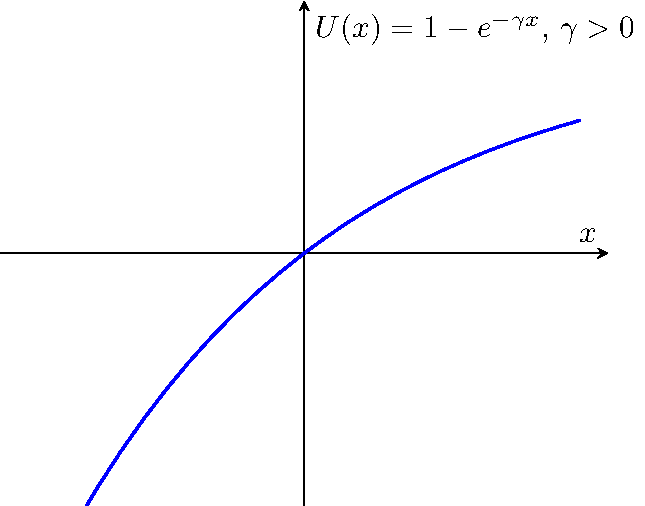
\includegraphics[width=0.35\linewidth]{Control_lecture_notes/Figs/utility1.pdf}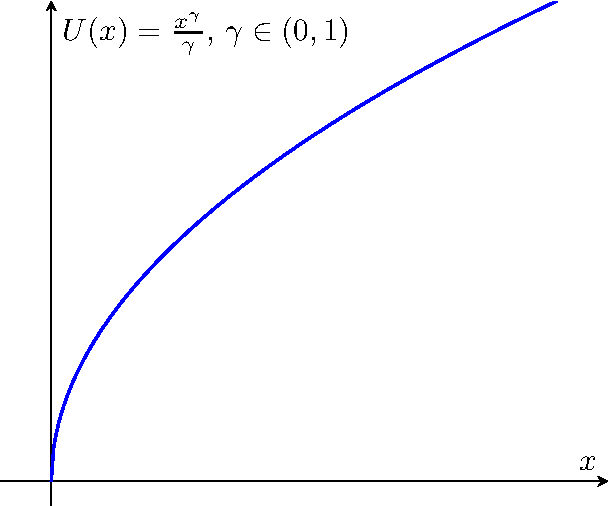
\includegraphics[width=0.35\linewidth]{Control_lecture_notes/Figs/utility2.pdf}
            \caption{Utility functions: left $U(x)=1-e^{-\gamma x}$, right $U(x)=\frac{x^{\gamma}}{\gamma}$}
            \label{fig:utilities}
        \end{figure}
        
        Derive the HJ equation for this problem.
\end{ex}

\begin{ex}\label{ex:consumption_no_terminal}
    In the above exercise, if we ignore the terminal gain, we obtain 
    \[
        {\color{orange}\sup_{c_t\ge0}}\int_0^T U(c_t)\dt,~~\dd{X}_t = (rX_t - c_t)\dt
    \]
    Is there something wrong with this problem? What stops us from consuming infinite amount and go negative on the wealth?

    If we restrict the consumption to maintain a positive balance, $X_t\ge0$ for all $t$, does the issue go away?
\end{ex}
%%%%%%%%%%%%%%%%%%%%%%%%%%%%%%%
\subsubsection{Exponential decay in control problems}
We consider the case where, $C(t,x,u)={\color{blue}e^{-r t}}\bar{C}(u,x)$ and $f(t,x,u)=f(x,u)$
\begin{equation}
\label{prob:deterministic_decay}
    \inf_{u}\int_0^T e^{-k t}\bar{C}(u_t,x_t)\dt + {\color{blue}e^{-k T}}g(x_T),~~\dx_t=f(x_t,u_t)\dt
\end{equation}
The \emph{exponential decay} term, ${\color{blue}e^{-kt}}$ emphasized on the importance of cost functions relative to the starting time. As time grow, the contribution of a unit of cost decreases. This is a common practice in applications from economics. While we can write the value function and the dynamic programming principle the same way as \eqref{eqn:value_deterministic} and \eqref{eqn:dpp_deterministic}, we can slightly modify the definition of value function and simplify the DPP and the HJ equation.
\begin{defn}
The value function of \eqref{prob:deterministic_decay} for $x_t=x$ is defined by
\begin{equation}\label{eqn:value_deterministic_decay}
    V(t,x):= \inf_{u\in\mathcal{U}_{t}}\int_t^Te^{-k(s-t)}\bar{C}(x_s,u_s){{\ds}}+e^{-k(T-t)}g(x_T),~~~~{\dx}_s=f(x_s,u_s){{\ds}}
\end{equation}
where $\mathcal{U}_{t}$ is the set of admissible controls restricted to time interval $[t,T]$.
\end{defn}
The dynamic programming principle is modified by:
\begin{thm}\label{thm:dpp_deterministic_decay}
    [Dynamic Programming Principle]
    Let $0\le t<s\le T$ and $x_t=x$. Then, the DPP for \eqref{prob:deterministic_control} is given by 
    \begin{equation} \label{eqn:dpp_deterministic_decay}
    V(t,x) =\inf_{u\in\mathcal{U}_{t,s}}\int_t^s e^{-k(r-t)}\bar{C}(x_r,u_r){{\dr}}+e^{-k(s-t)}V(s,x_s),~~~~{\dx}_r=f(x_r,u_r){{\dr}}
\end{equation}
where $\mathcal{U}_{t,s}$ is the set of admissible controls restricted to time interval $[t,s]$.
\end{thm}
\begin{proof}
    The proof is quite similar to Theorem~\ref{thm:dpp_deterministic}.
\end{proof}
    We apply Taylor series on $e^{-k(s-t)}V(s,x_s)$ around $(t,x)$.
    \[
        \begin{split}
             {e^{-k(s-t)}}V(s,x_s) = &V(t,x) + {e^{-k(s-t)}}\Big(\big(V_t(t,x) {- k V(t,x)}\big)(s-t)\\
             &~~~~+ V_x(t,x)\cdot\int_t^s f(x_r,u_r)\dr\Big) + o((s-t)^2)
        \end{split}
        \]
       We use Taylor series inside \eqref{eqn:dpp_deterministic_decay} to write
        \[
        \begin{split}
            0=\inf_{u}\int_t^s &{e^{-k(r-t)}}\bar{C}(x_r,u_r)\dr \\
            &+  {e^{-k(s-t)}}\Big(\big(V_t(t,x) {- k V(t,x)}\big)(s-t)\\
             &~~~~+ V_x(t,x)\cdot\int_t^s f(x_r,u_r)\dr\Big) + o((s-t)^2)
        \end{split}
        \]
        Dividing both sides by $s-t$ and sending $s\to t$ yields the HJ equation.
        \begin{equation}
            \label{eqn:HJ_deterministic_decay}
            0=V_t(t,x) - k V(t,x)+\inf_{u}\Big\{\bar{C}(x,u) + V_x(t,x)\cdot f(x_r,u_r)\Big\}
        \end{equation}
        The term ${\color{blue}-kV}$ in the HJ equation is coming from the discounting. 
        The boundary (terminal) condition remains the same, $V(T,x)=g(x)$. 
        \begin{equation}
        \label{eqn:HJ_decay_w_Hamiltonian}
            \begin{cases}
                0=V_t(t,x) - k V(t,x)+H(x,V_x)\\
                V(T,x)=g(x)
            \end{cases}
        \end{equation}
        with
        \[
        H(x,p)=\inf_{u}\Big\{\bar{C}(x,u) + p\cdot f(x_r,u_r)\Big\}
        \]
        The relation between the HJ equation with decay term in \eqref{eqn:HJ_deterministic_decay} and the HJ equation in \eqref{eqn:HJ_deterministic} can easily be verifies by the change of variable $\bar{V}(t,x)=e^{k(T-t)}V(t,x)$. $V(t,x)$ satisfies \eqref{eqn:HJ_decay_w_Hamiltonian} if and only if $\bar{V}(t,x)$ satisfies \eqref{eqn:HJ_w_Hamiltonian}. 
        \begin{ex}
            Show that $V(t,x)$ satisfies \eqref{eqn:HJ_decay_w_Hamiltonian} if and only if $\bar{V}(t,x)$ satisfies \eqref{eqn:HJ_w_Hamiltonian}. 
        \end{ex}
    
    A good question to ask ourselves is that for Problem \eqref{prob:deterministic_decay} if the the HJ equation with or without decay term can be obtained via a simple change of variable, why do we introduce a different value function and DPP for exponential decay?
    The answer lies in the case when $T=\infty$:
    \begin{equation}
    \label{prob:deterministic_decay_infinite}
        \inf_{u}\int_0^\infty e^{-k t}\bar{C}(u_t,x_t)\dt ,~~\dx_t=f(x_t,u_t)\dt
    \end{equation}
    Since $f(x_t,u_t)$ does not depend on $t$, the solution $x_s$ of ${\dx}_s=f(x_s,u_s){\ds}$ with $x_t=x$ is the same as a time shift of $\bar{x}_r$ the solution of ${\dx}_r=f(x_r,u_r){\ds}$ with $x_0=x$ by $t$.
    \[
        V(t,x)= \inf_{u\in\mathcal{U}_{t}}\int_t^\infty e^{-k(s-t)}\bar{C}(x_s,u_s){{\ds}}{{\ds}}=\inf_{u\in\mathcal{U}}\int_0^\infty e^{-kr}\bar{C}(\bar{x}_{r},u_{r}){{\dr}}
    \]
    Therefore, value function is time homogeneous
    and is given by
    \begin{equation} \label{eqn:value_decay_infinite}
    V(x)=\inf_{u\in\mathcal{U}}\int_0^\infty e^{-kr}\bar{C}(\bar{x}_{r},u_{r}){{\dr}}
    \end{equation}
    and the HJ equation is given by 
    \begin{equation} \label{eqn:HJ_decay_w_Hamiltonian_homogeneous}
                0=- k V(t,x)+H(x,V_x)            
    \end{equation}
    \begin{ex}
    Consider the consumption problems, Exercise~\ref{ex:consumption} and Exercise~\ref{ex:consumption_no_terminal}, in infinite horizon with decay term:
    \[
        {\sup_{c_t\ge0}}\int_0^\infty e^{-kt}U(c_t)\dt,~~\dd{X}_t = (rX_t - c_t)\dt
    \]
    Here, set of admissible consumption are those such that we maintain $X_t\ge0$ for all $t\ge0$. Write the value function by using \eqref{eqn:value_decay_infinite} and the HJ equation by \eqref{eqn:HJ_decay_w_Hamiltonian_homogeneous}. Find proper boundary condition and solve the HJ equation with the boundary condition.
    \end{ex}
        
%%%%%%%%%%%%%%%%%%%%%%%%%%%%%%%
\subsection{An introduction to viscosity solution}
To motivate viscosity solutions, we introduce the following example.
\begin{eg}
\label{eg:eikonal_2}
    Recall from Exercise~\ref{ex:eikonal} that
    \[
        \inf_u\int_0^\infty \mathds{1}_{\{x_t\in D\}}{\dt},~{\dx}_t=u_t{{\dt}}~\text{ with }~|u_t|\le1
    \]
    The value function for initial state $x_0=x\in D$ is given by
    \[
        V(x)=\inf_u\int_0^\infty \mathds{1}_{\{x_t\in D\}}{\dt},~{\dx}_t=u_t{{\dt}}~\text{ with }~|u_t|\le1
    \]
    Here $C(x,u)=C(x)=\mathds{1}_{\{x\in D\}}$ and $f(x,u)=f(u)=u$.
    Notice that the value function \emph{does not} depend on $t$, because the total cost is a function of duration of time until exit and not the function of current time.

    The HJ equation is given by
    \[
    H(V_x)=0,~~~H(x,p):=\inf_{|u|\le1}\{\mathds{1}_{\{x\in D\}}+p\cdot u\}
    \]
    We can restrict the Hamiltonian to points $x\in D$ and write 
    \[
    H(p):=\inf_{|u|\le1}\{1+p\cdot u\}=1+\inf_{|u|\le1}\{p\cdot u\}
    \]
    The infimum above is attained for $u=-\frac{u}{|u|}$. Therefore,
    \[
    H(p)=|p|
    \]
    Outside (or on the boundary of) $D$, the exit time is zero. Therefore, we restrict the Hamiltonian to inside of the domain and impose the boundary condition $V(x)=0$ for $x\in\partial D$. We conclude that the HJ equation with the boundary condition is given by
    \[
    \begin{cases}
        1-|V_x|=0&x\in D\\
        V(x)=0&x\in \partial D
    \end{cases}
    \]
\end{eg}
Example~\ref{eg:eikonal_2} can shed a light on the notion of solution to the HJ equations. Take $D=[-1,1]\subset \mathbb{R}$ and consider the following functions,  shown in Figure~\ref{fig:v1v2}:
        \[
        v_1(x) = 1-|x|, v_2(x)= \begin{cases}
            \frac12-|x-\frac12|&0\le x\le1\\
            \frac12-|x+\frac12|&-1\le x<0
        \end{cases}
        \]
The minimal exit time of $[-1,1]$ is given by $v_1$. Additionally, except at point $x=0$, $v_1$ is differentiable, satisfies the HJ equation, and the optimal direction and speed is given by $V_x=\text{\normalfont sgn}(x)$. $v_2$ is not the value function  , but it also satisfies the HJ equation except at three points, $x=0,\pm\frac12$. 
 In fact, with a little bit of effort, one can write infinitely many solutions for the Eikonal equations. All this solutions have points of non-differentiability. However, the right and the left derivatives at those points still satisfy the HJ equation. 
\begin{figure}
    \centering
    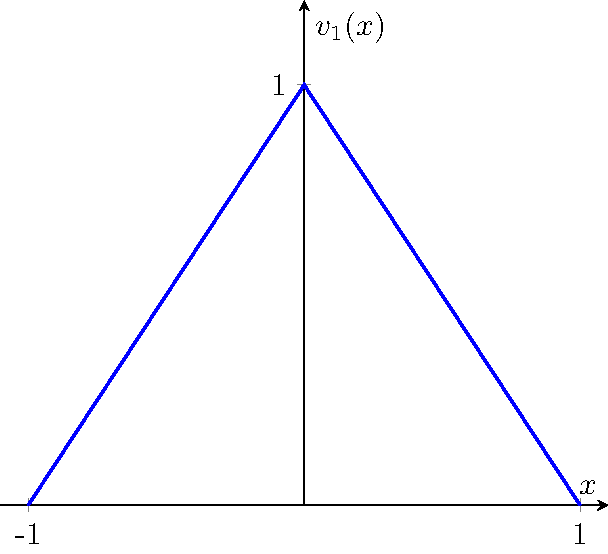
\includegraphics[width=0.25\linewidth]{Control_lecture_notes/Figs/v1.pdf}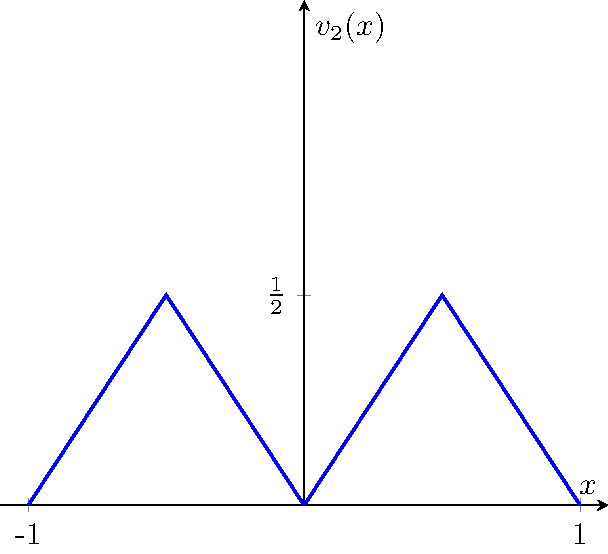
\includegraphics[width=0.25\linewidth]{Control_lecture_notes/Figs/v2.pdf}
    \caption{Functions $v_1$ and $v_2$ solve Eikonal equation, the HJ equation for \ref{eg:eikonal_2}. But, only  $v_1$ is the same as the value function.}
    \label{fig:v1v2}
\end{figure}
That raises an issue; \emph{if we solve an HJ equation, how do we know if we obtained the correct solution, hence, the value function?} The answer to this problem is quite complicated. The theory that solves the issue is the theory of \emph{viscosity solutions}, which we discuss in more details in a later chapter. Here, we explain a simpler version of this theory by focusing on the Eikonal equation, $0=1-|v^{\prime}(x)|$ with boundary condition $v(-1)=v(1)=0$. 

We introduce a new equation by adding a second order term. 
\[
0=1-|v^{\epsilon\prime}(x)|+\epsilon V^{\epsilon\prime\prime}, ~~ v^{\epsilon}(-1)=v^{\epsilon}(1)=0
\]
The above equation is a second order equation with two boundary conditions, which guarantees existence of a unique differentiable solution which can be found in closed form by solving
\[
\begin{cases}
    0=1+v^{\epsilon\prime}(x)+\epsilon V^{\epsilon\prime\prime}& x\in(0,1)\\
    0=1-v^{\epsilon\prime}(x)+\epsilon V^{\epsilon\prime\prime}& x\in(-1,0)\\
    v^{\epsilon\prime}(0)=0&\\
    v^{\epsilon}(0-)=v^{\epsilon}(0+)&\\
    v^{\epsilon}(-1)=v^{\epsilon}(1)=0
\end{cases}
\]
\begin{ex}
    Find a closed form solution. above system of equations.
\end{ex}
Then, if we evaluate $\lim_{\epsilon\to0}v^{\epsilon}$, we obtain $v_1=V$.

\citet{CIL92}, codified the above construction into the theory of viscosity solutions, which perfectly fits the need of HJ equations in optimal control. For the points of non-differentiability, they introduces candidates for  derivative from above and from below. More precisely, they defined the set of \emph{superjets} as the slope of all lines that touch the function from above and the set of \emph{subjets} as the slope of all lines that touch the function from below, as shown in Figure~\ref{fig:jets}.

\begin{figure}
    \centering
    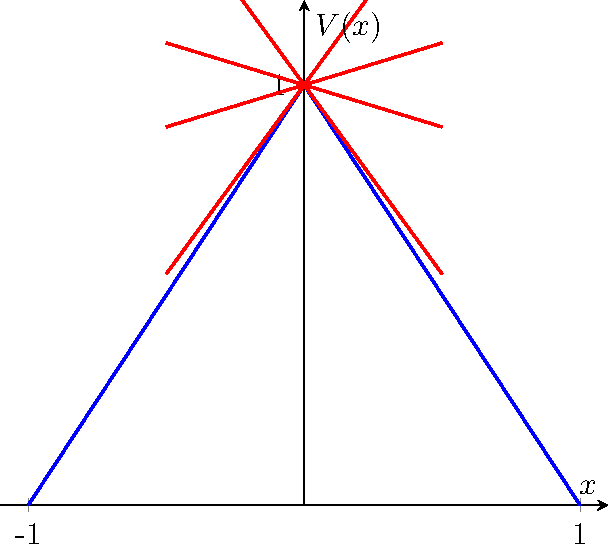
\includegraphics[width=0.35\linewidth]{Control_lecture_notes/Figs/superjets.pdf}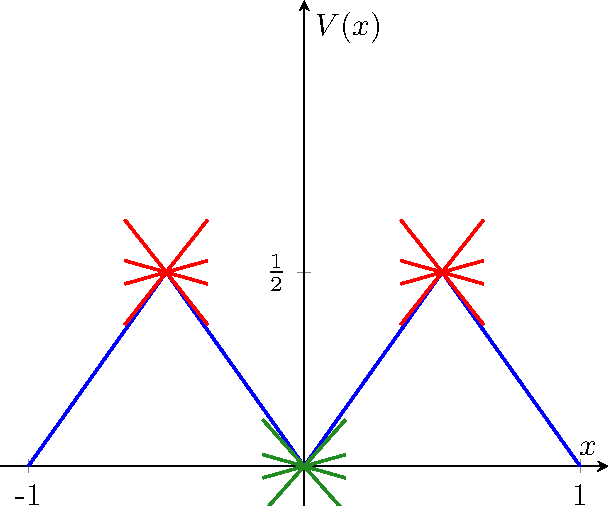
\includegraphics[width=0.35\linewidth]{Control_lecture_notes/Figs/jets.pdf}
    \caption{Superjets and subjets for functions $v_1$ and $v_2$ at the points of non-differentiability.}
    \label{fig:jets}
\end{figure}
The set of superjets, $\overline{J}$, and subjets, $\underline{J}$, for all the points of non-differentiability are the closed interval $[-1,1]$. According to the theory of viscosity solutions, the members of superjet must satisfy the equation with inequality:
\[
\forall a\in\overline{J}=[-1,1], 1-|a| \ge 0
\]
which is trivially correct for for $v_1$ at $x=0$ and for $v_2$ at $x=\frac12=-\frac12$.
Similarly,  the members of subjet must satisfy the equation with inequality in the opposite direction of superjets:
\[
\forall a\in\underline{J}=[-1,1], 1-|a| \le 0.
\]
However, for $v_2$ at $x=0$, $a\in\underline{J}=(-1,1)$ $1-|a| \not\le 0$. Therefore, $v_2$ is not a viscosity solution of the eikonal equation.

Interesting results from the theory of viscosity solution are as follows.
\begin{enumerate}[label=\arabic*)]
    \item The value function of a control problem is a viscosity solution of the HJ equation.
    \item HJ equation has a unique viscosity solution.
    \item Numerical solutions to HJ equations with certain standard properties converge to the viscosity solution.
\end{enumerate}
Even though there are more details into these results, we continue to use these results in this note until we require more clarifications.

\subsection{Summary}
The steps of solving deterministic control problems via HJ problem are described in Chart~\ref{fig:chart1}:
\begin{figure}[ht!]
    \centering
    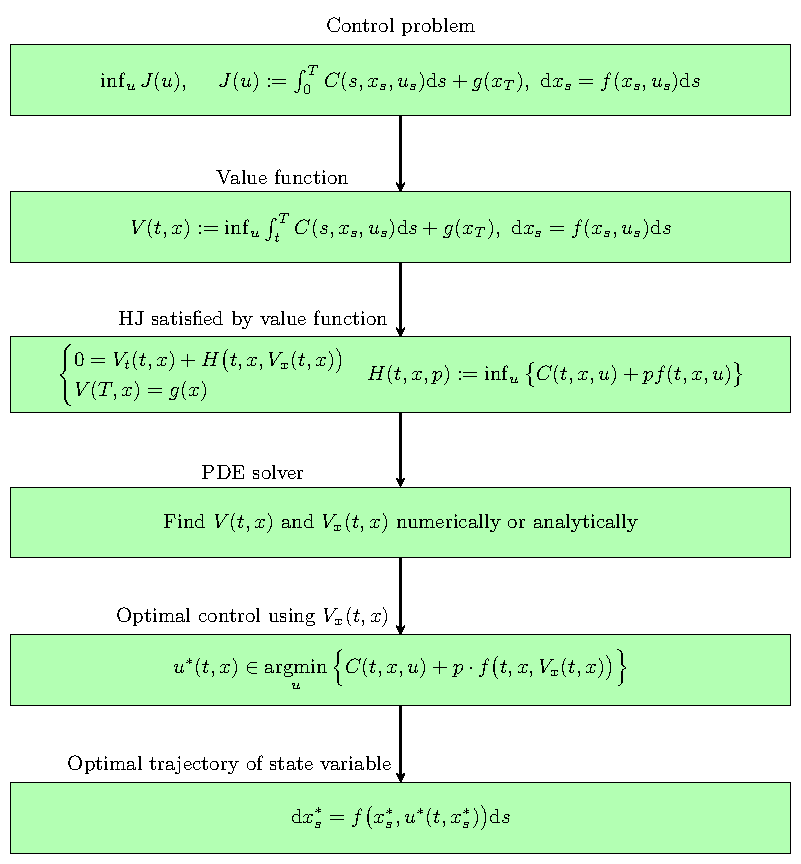
\includegraphics[height=0.5\textheight]{Control_lecture_notes/Figs/HJ_chart.pdf}
    \caption{Summary of HJ solution method for control problems}
    \label{fig:chart1}
\end{figure}
It is important to note that when the HJ equation is derived, solving HJ equation is an standalone problem. After solving the HJ equation, the solution and its derivatives are used to find an optimal control and the corresponding optimal trajectory.
%%%%%%%%%%%%%%%%%%%%%%%%%%%%%%%

\subsection{Pontryagin principle}
\label{sec:det_pontryagin}
Consider the simple control problem in Section~\ref{sec:opt_control}:
\begin{equation}
\inf_{u}\bigg\{\int_0^T\Big(x_t^2 - \alpha_t x_t\Big) {{\dt}}\bigg\}
\end{equation}
where ${\dx}_t = (-\beta x_t + u_t ){{\dt}}$, $x_0=x$.
One can consider the dynamics of $x$ as a constraint. Therefore, we can formally write Lagrangian by 
\begin{equation}\label{ex:sup_inf}
    \sup_{\lambda}\inf_{u,x}\bigg\{\int_0^T\big(x_t^2 - \alpha_t x_t\big) {{\dt}} - \int_0^T \lambda_t \big({\dx}_t + (\beta x_t  - u_t ){{\dt}}\big)\bigg\}
\end{equation}
Here, there are two important remarks. First,
 since the constraint is given by a differential equation for each $t$, the dual variable $\lambda$ is a function of $t$. Second, the problem is now unconstrained, that is, the state variable $x$ and the control variable $u$ are now both  variables in an optimization problem.
 
The main trick to solve this optimization problem is integration by part formula
\begin{equation}\label{eqn:pontryagin_ibp}
    \int_0^T \lambda_t {\dx}_t = \lambda_T x_T - \lambda_0 x_0 - \int_0^T x_t{\dd}\lambda_t
\end{equation}
to write 
\eqref{ex:sup_inf} as
\begin{equation}\label{ex:pontryagin}
    \sup_{\lambda}\inf_{u,x}\bigg\{\int_0^T\Big(x_t {\dd}\lambda_t-\lambda_t( \beta x_t - u_t )+ x_t^2 - \alpha_t x_t \Big) {{\dt}} - \lambda_T x_T + \lambda_0 x_0\bigg\}
\end{equation}
Note that optimization on $x_T$ is independent of  $x_t$ for $t<T$. The KKT conditions for the strong duality in the saddle point problem \eqref{ex:pontryagin} were discovered by Lev Pontryagin in 1952. Define the \emph{Hamiltonian} by
\begin{equation}
    H(t,x,\lambda,u):=-\lambda( \beta x - u )+ x^2 - \alpha_t x
\end{equation}
Thus, \eqref{ex:pontryagin} is written as a saddle point problem with free variables $x_t$, $u_t$, and $\lambda_t$:
\begin{equation}
    \sup_{\lambda}\inf_{u,x}\bigg\{\int_0^T\Big(x_t {\dd}\lambda_t+ H(t,x_t,\lambda_t,u_t)\Big) {{\dt}} - \lambda_T x_T + \lambda_0 x_0\bigg\}
\end{equation}
\begin{equation}
    \begin{cases}
        {\dd}\lambda^*_t+ \partial_x H(t,x^*_t,\lambda^*_t,u^*_t){{\dt}}={\dd}\lambda^*_t+ (-\lambda^*_t \beta  +2x^*_t -\alpha_t){{\dt}}=0~ (\textrm{minimize integrand wrt $x$})\\
        \lambda^*_T=0 ~(\textrm{minimize terminal wrt $x_T$})\\
        H(t,x^*_t,\lambda^*_t,u^*_t)\le H(t,x^*_t,\lambda^*_t,u)~\textrm{ for all } u ~(\textrm{minimize integrand wrt $u$})\\
        {\dx}^*_t = (-\beta x^*_t + u^*_t) {{\dt}} ~(\textrm{constraint})
        \end{cases}
\end{equation}
In the above, the first equation  is obtained from taking derivative with respect to $x_t$, second equality corresponds to derivative with respect to $x_T$ in $\lambda_T x_T$, the third line guarantees the optimality of $u^*$, and the last equation is the  constraint of the problem which is the dynamic of the state variable in the control. 
\begin{ex}
    Show that $\lambda^*_t=0$, $x^*_t=\alpha_t/2$, and $u^*$ with $\alpha_t=2\int_0^te^{-\beta (s-t)}u^*_s {{\ds}}$ satisfy Pontryagin principle for the above problem. 
\end{ex}

Following the steps of in the above example, the Pontryagin principle for a generic deterministic control problem, \ref{prob:deterministic_control} is described as the following saddle point problem.
\begin{equation}\label{eqn:sup_inf}
    \sup_{\lambda}\inf_{u,x}\bigg\{\int_0^TC(t,x_t,u_t) {{\dt}} +g(x_T) - \int_0^T \lambda_t \big({\dx}_t + (\beta x_t  - u_t ){{\dt}}\big)\bigg\}
\end{equation}
By applying \eqref{eqn:pontryagin_ibp}, we obtain 
\begin{equation}
    \sup_{\lambda}\inf_{u,x}\bigg\{\int_0^T\Big(x_t {\dd}\lambda_t+ H(t,x_t,\lambda_t,u_t)\Big) {{\dt}} +g(x_T) - \lambda_T x_T + \lambda_0 x_0\bigg\}
\end{equation}
where the Hamiltonian is given by 
\begin{equation}
    H(t,x,\lambda,u):=\lambda f(t,x,u)+ C(t,x,u)
\end{equation} 
\begin{thm}\label{thm:pontryagin_deterministic}
    [Pontryagin principle]
    Assume that there exists $(x^*,u^*,\lambda^*):[0,T]\to\mathbb{R}^d\times\mathbb{R}^n\times\mathbb{R}^d$ such that
    \begin{equation}\label{eqn:pontryagin_determinimstic}
    \begin{cases}
        {\dd}\lambda^*_t+ \partial_x H(t,x^*_t,\lambda^*_t,u^*_t){{\dt}}=0~ (\textrm{minimize integrand wrt $x$})\\
        \lambda^*_T=\nabla g(x^*_T) ~(\textrm{minimize terminal wrt $x_T$})\\
        H(t,x^*_t,\lambda^*_t,u^*_t)\le H(t,x^*_t,\lambda^*_t,u)~\textrm{ for all } u ~(\textrm{minimize integrand wrt $u$})\\
        {\dx}^*_t = f(t,x^*_t,u^*_t) {{\dt}} ~(\textrm{constraint})
        \end{cases}
\end{equation}
Then, $u^*$ is an optimal control for \eqref{prob:deterministic_control}.
\end{thm}
% Assume that $u^*$ is \emph{an} \emph{optimal control} for \ref{prob:deterministic_control} and  $x^*$ is \emph{the} optimal trajectory for $u^*$, i.e., ${\dx}^*_t = f(t,x^*_t,u^*_t) {{\dt}}$.
% Then, there exists $\lambda^*$ such that 
% \begin{equation}
%     \begin{cases}
%         {\dd}\lambda^*_t+ \partial_x H(t,x^*_t,\lambda^*_t,u^*_t){{\dt}}=0\\
%         \lambda^*_T=\triangledown g(x^*_T)\\
%         H(t,x^*_t,\lambda^*_t,u^*_t)\le H(t,x^*_t,\lambda^*_t,u)~\textrm{ for all } u
%         \end{cases}
% \end{equation}
The function $\lambda^*_t$, described by \ref{thm:pontryagin_deterministic} is called the \emph{adjoint} process. It is important to distinguish between the two ODEs in \eqref{eqn:pontryagin_determinimstic}, namely, 
\begin{equation}
    {\dx}^*_t = f(t,x^*_t,u^*_t) {{\dt}} \text{ and }{\dd}\lambda^*_t+ \partial_x H(t,x^*_t,\lambda^*_t,u^*_t){{\dt}}=0
\end{equation}
The first one has an initial condition $x^*_0=x_0$, the initial position of the state process. However, the adjoint equation comes with a terminal condition, $\lambda^*_T=\nabla g(x^*_T)$. This makes solving Theorem~\ref{thm:pontryagin_deterministic} challenging. We shall see later how Pontryagin principle is applied to some specific examples such as linear quadratic linear control problem, where solving \eqref{eqn:pontryagin_determinimstic} is simpler to solve. 
\begin{rem}
If $u^*_t$ is an interior minimizer of $H(t,x^*_t,\lambda^*_t,u)$, then we can write $\partial_u H(t,x^*_t,\lambda^*_t,u^*_t)=0$. However, if there are constraint on $u$, e.g., $u\ge0$, we shall stick to the inequality above. 
\end{rem}

We start with an example of a LQC problem. 
\begin{eg}\label{eg:lqc}
    Consider the control problem with $C(x,u)= x^2 +  u^2$, $g(x) = x^2 +  x$, and $f(x,u)=x + u$:
\begin{equation}
    \inf_{u}\int_0^T(x_t^2 + u_t^2 ){{\dt}} + x^2_T + x_T,~\text{ subject to  }~{\dx}_t=( x_t +  u_t){{\dt}}
\end{equation}
\end{eg}
LQC problems can be solved via Pontryagin principle. More precisely,  for the above example, the Hamiltonian is given by
\[
H(x,\lambda,u) = x^2 + u^2 + \lambda ( x + u)
\]
and \eqref{eqn:pontryagin_determinimstic} is 
\begin{equation}\label{eg:pontryagin_lqc}
    \begin{cases}
        {\dd}\lambda^*_t+ (2x^*_t + \lambda^*_t ){{\dt}}=0\\
        \lambda^*_T= 2x^*_T + 1\\
        H(t,x^*_t,\lambda^*_t,u^*_t)\le H(t,x^*_t,\lambda^*_t,u)\\
        {\dx}^*_t=( x^*_t + u^*_t){{\dt}}
        \end{cases}
\end{equation}
Minimizing $H(x,\lambda,u)$ in $u$ suggests that $H_u(x,\lambda^*_t,u^*_t)=2u^*_t+  \lambda^*_t =0$, equivalently, $u^*_t=-\frac{1}{2}\lambda^*_t$.
\begin{ex}
    (1) Use $u^*_t=-\frac{1}{2}\lambda^*_t$ to write the system of ODEs \eqref{eg:pontryagin_lqc} for $\lambda^*$ and $x^*$ by
    \begin{equation}
        \begin{cases}
        {\dd}\lambda^*_t= (- \lambda^*_t - 2x^*_t){{\dt}}\\
        {\dx}^*_t=( -\frac12\lambda^*_t+x^*_t  ){{\dt}}
        \end{cases}
    \end{equation}
    (2) Find the general solution the system of ODEs in terms of $x^*_0$ and $\lambda^*_0$. Hint: Use denationalization of the matrix 
    \begin{equation}
        \left[
        \begin{matrix}
            -1&-2\\
            -\frac12&1
        \end{matrix}
        \right] =\left[\begin{matrix}2(\sqrt2+1)&1\\1&2(\sqrt2-1)\end{matrix}\right] \left[\begin{matrix}-\sqrt{2}&0\\0&\sqrt{2}\end{matrix}\right] \left[\begin{matrix}\frac23(\sqrt2-1)&-1\\-1&\frac23(\sqrt2+1)\end{matrix}\right]
    \end{equation}
    and write the ODEs as 
    \begin{equation}
        \left[\begin{matrix}{\dd}\lambda^*\\{\dx}^*\end{matrix}\right] = \left[
        \begin{matrix}
            1&1\\
            1&-\frac12
        \end{matrix}
        \right] 
        \left[\begin{matrix}\lambda^*\\x^*\end{matrix}\right] = \left[\begin{matrix}2(\sqrt2+1)&1\\1&2(\sqrt2-1)\end{matrix}\right] \left[\begin{matrix}-\sqrt{2}&0\\0&\sqrt{2}\end{matrix}\right] \left[\begin{matrix}\frac23(\sqrt2-1)&-1\\-1&\frac23(\sqrt2+1)\end{matrix}\right]\left[\begin{matrix}\lambda^*\\x^*\end{matrix}\right]
    \end{equation}
    (3) Consider $x^*_0$ given. Use $\lambda^*_T= 2x^*_T + 1$ to find $\lambda^*_0$, hence a special solution for the system of ODEs from Pontryagin principle as a function $x^*_0$ and $x^*_T$.  
\end{ex}
%%%%%%%%%%%%%%%%%%%%%%%%%%%%%%%
\section{Linear quadratic control problem}
\label{sec:LQC}
A class of control problem with closed-form solution consists of \emph{linear-quadratic} optimal control problems, LQC henceforth. 
In LQC, the running cost is quadratic in $x$ and $u$, the terminal cost is quadratic in $x$, and the ODE for state variable is linear in $x$ and $u$. We assume that $x$ is a $d$-dimensional column vector and $u$ is an $m$-dimensional column vector.
\begin{equation}
    \begin{split}
        &C(t,x,u) = \left[\begin{matrix}
        x^\top&
        u^\top
        \end{matrix}\right]Q_t\left[\begin{matrix}
        x\\
        u
        \end{matrix}\right]+a_t\cdot x + b_t\cdot u,~\text{ and }~Q_t=\left[\begin{matrix}
        A_t&C_t\\
        C_t^\top&B_t
        \end{matrix}\right]\\
        &g(x) = x^\top A_T x+a_T \cdot x\\
        &f(t,x,u) = M_t x + N_t u
    \end{split}
\end{equation}
Here, $A:[0,T]\to \mathbb{M}(d,d)$, $B:[0,T]\to \mathbb{M}(m,m)$, $C:[0,T]\to \mathbb{M}(d,m)$, $a:[0,T]\to \mathbb{R}^d$, $b:[0,T]\to \mathbb{R}^m$, $M:[0,T]\to \mathbb{M}(d,d)$, and $N:[0,T]\to \mathbb{M}(d,m)$. 


For LQC problem to be well-posed, the value is not $-\infty$, it is sufficient to assume that $Q_t$ and $A_T$ are symmetric and positive definite. In this case $C$ and $g$ are convex functions of $(x,u)$ and $x$, respectively. See exercise below.
\begin{ex}
    In Example~\ref{eg:lqc}, change the running cost function to $C(x,u)= x^2 -  u^2$. Make some effort to find a solution to this modified problem. Of course, since the cost function is not convex, your effort fails. Explain why the optimal control problem is ill-defined.
\end{ex}

\begin{ex}
    Write the HJB equation for the LQC problem.
\end{ex}

\begin{ex}
Assume that the cost functions of the general LQC problem are convex.
    Verify that there exists $G:[0,T]\to \mathbb{M}(d,d)$, $H:[0,T]\to \mathbb{R}^d$, and $K:[0,T]\to \mathbb{R}$ such that 
    $V(t,x) = x^\top G_t x + H_t\cdot x + K_t$ satisfied the HJ equation.
\end{ex}


\begin{ex}
Assume that the cost functions of the general LQC problem are convex.
    Write Pontryagin principle for the general LQC and suggest a solution method. 
\end{ex}


%%%%%%%%%%%%%%%%%%%%%%%%%%%%%%%
%%%%%%%%%%%%%%%%%%%%%%%%%%%%%%%
%%%%%%%%%%%%%%%%%%%%%%%%%%%%%%%
%%%%%%%%%%%%%%%%%%%%%%%%%%%%%%%
\chapter{Stochastic Control}
We explain the components of a stochastic control problem.
\section{State process}
Given a progressively measurable process\footnote{A process is called progressively measurable if for any $t$, the restriction to $[0,t]\times\Omega$ is $\mathcal{B}[0,t]\otimes\mathcal{F}_t$-measurable.} $u_t$ taking values in a set $\mathbf{U}\subseteq \mathbb{R}^m$, which will be clarified later, the state process is given by the SDE
\begin{equation}\label{eqn:state_process}
	\begin{cases}
	    {\dx}^u_t =\mu(t,X_t^u,u_t){{\dt}}+\sigma(t,X_t^u,u_t){\dd}B_t\\
     X^u_0=x\in\mathbb{R}^d
	\end{cases}
\end{equation}
\begin{rem}
    If we assume that $\mu(t,x,u)$ and $\sigma(t,x,u)$ are Lipschitz continuous in $(t,x)$ uniformly in $u$, i.e.,
    \begin{equation}
       \sup_{u\in\mathbf{U}}\{ |\mu(t,x,u)-\mu(s,y,u)|+|\sigma(t,x,u)-\sigma(s,y,u)|\}\le K(|t-s|+|x-y|)
    \end{equation}
    Then for any progressively measurable $u_t$, \eqref{eqn:state_process} has a \underline{strong} solution.
\end{rem}
\begin{rem}
    In the deterministic control, $\sigma\equiv0$.
\end{rem}

\begin{eg}
	Take $u\equiv0$ in ${\dX}^u_t=u_tX_t^u {{\dt}}$. Then, $X_t^0=X_0$. For $u\equiv 1$, $X_t^1=X_0e^t$ and For $u_t=-t$, $X_t^u=X_0e^{-t^2/2}$. In general, $X_t^u=X_0e^{\int_0^tu_s{{\ds}}}$.
\end{eg}
\begin{eg}\label{eg:wealth}
In Black-Scholes model, the price of an asset satisfies ${{\ds}}_t=S_t(\mu {{\dt}}+\sigma {\dd}B_t)$. If the interest rate $r=0$ and $u_t$ is the amount of money invested in the asset, the wealth process from a self-financing portfolio satisfies
	\begin{equation}
	    {\dX}^u_t=u_t(\mu {{\dt}}+\sigma {\dd}B_t)
	\end{equation} 
 Then, $X_t^u=X_0\exp\big(\sigma\int_0^tu_s{\dd}B_s+(\mu-\sigma^2/2)\int_0^t u^2_s{{\ds}}\big)$, where $X_0$ is the initial wealth.
	\end{eg}
\section{Objective function}
The goal is to  minimize (or maximize) an objective function of the following form. Set $X_0^u=x$ for all $u$ and define
\begin{equation}
J(x;u)=\mathbb{E}\left[\int_0^T C(s,X_s^u,u_s){{\ds}}+g(X_T^u)\right].
\end{equation}
where $C:[0,T]\times\mathbb{R}^d\times\mathbb{R}^m\to\mathbb{R}$ is called running cost and $g:\mathbb{R}^d\to\mathbb{R}$ is the terminal cost. 
We assume that $C(t,x,u)$ is Lipschitz in $(t,x)$ uniformly in $u$ and $g$ is Lipschitz. Here, we only focus on minimization as minimization can be obtained by a negative sign. 


The value of the problem is
\begin{equation}
	V:=\inf_{u}J(x;u).
\end{equation}
If a process $u^*$ exists such that   $V=J(x;u^*)$, we call $u^*$ and optimal control. 

%%%%%%%%%%%%%%%%%%%%%%%%%%
\section{Admissibility}
It is easy to model stochastic control problems from real applications.  However, if not carefully done, the stochastic control problem becomes degenerate.

\begin{ex}[St. Peterburg paradox]\label{eg:admissibility_paradox}
	Consider the wealth process as described by \eqref{eg:wealth} and assume that asset price $S$ is a martingale by setting $\mu=0$.
 In this case, $X_t=X_0+\sigma\int_0^tu_s{\dd}B_s$. Further, assume $X_0=0$.
 Let's try to maximize expected value of wealth by applying an investment strategy $u$:
 \begin{equation}\label{st.petersburg}
     V = \sup_{u}\mathbb{E}[X_T^u]=\sigma\sup_{u}\mathbb{E}\bigg[\int_0^T u_s{\dd}B_s\bigg].
 \end{equation}
 Is the stochastic integral above zero? Why?

 Now, consider the strategy that chooses $u_t=u>0$, where $u$ is large and liquidate the investment as soon as $X_t^u=M$. If $X_t^u$ never hits $M$, the investment yields $X_T^u$.
 
Note that for $X^u_t=\sigma u B_t$, probability of hitting $M$ before $T$ is
\begin{equation}
    \mathbb{P}\big(\max_{t\le T} X_t^u\ge M\big) =  \mathbb{P}\bigg(\max_{t\le T} B_t\ge \frac{M}{\sigma u}\bigg) =  2\mathbb{P}\bigg(B_T\ge \frac{M}{\sigma u}\bigg)
\end{equation}
The last equality is coming from the Schwartz reflection principle for Brownian motion. If we send $u\to\infty$ and $M\to\infty$  such that $\frac{M}{u}\to0$, we obtain $\mathbb{P}(B_T\ge \frac{M}{\sigma u})\to \frac12$. 

On the other hand, from the strategy described above, we have 
\begin{equation}
    \mathbb{E}[X_T^u] = \mathbb{E}[M1_{\{\max_{t\le T} X_t^u\ge M\}}]+  \mathbb{E}[X_T^u1_{\{\max_{t\le T} X_t^u< M\}}]= 2M\mathbb{P}\bigg(B_T\ge \frac{M}{\sigma u}\bigg)+\mathbb{E}[X_T^u1_{\{\max_{t\le T} X_t^u< M\}}]
\end{equation}
Now, answer the following questions:
\begin{enumerate}
    \item Is it true that $\mathbb{E}[X_t^u1_{\{\max_{t\le T} X_t^u< M\}}]\to 0 $ as $u\to\infty$ and $M\to\infty$  such that $\frac{M}{u}\to0$?
    \item What is the limit of $2M\mathbb{P}(B_T\ge \frac{M}{\sigma u})$? $V=\infty$?
    \item If the stochastic integral in \eqref{st.petersburg} is zero, then $V=0$, why did we also get $V=\infty$?
\end{enumerate}





\end{ex}
The above example shows that if someone can have unlimited borrowing power, the value functions is infinite. From the practical point of view, this is not possible. If we define a set admissible controls to be all progressively measurable $u$ such that $c_t\ge0$ and $X_T^u\ge -C$  for some credit limit $C\ge0$\footnote{$C\ge0$ is no-short-selling condition.} $\mathbb{P}$-a.s., then the  strategies in Example~\ref{eg:admissibility_paradox} are not admissible.  

Another consideration is that the choice of control $u$ should be made such that the state process in \eqref{eqn:state_process} admits a solution for which $J(x;u)$ is defined and finite. For instance, in Example~\ref{eg:admissibility_paradox}, there are choices for $\theta_t$ such that ${\dX}_t=\sigma \theta_t {\dd}B_t$ does not have a (strong) solution, see \cite{tsirel1976example} for an example when strong solution does not exist. The set of admissible controls should be chosen such that it includes the (unknown) optimal control we are looking for. If too restricted, we would not get optimality; if two wide, we get bizaar solutions such as in St. Petersburg paradox, \ref{eg:admissibility_paradox}.

Based on the above discussion, we define the set of admissible controls for \ref{eg:admissibility_paradox} can be 
\begin{equation}\label{eqn:admissible}
	\begin{split}
		\mathcal{A}_C&=\Big\{u\ :  \mathbb{P}\textrm{-a.s.}, u~\textrm{is progressively measurable}, \textrm{SDE ${\dX}^u_t=\sigma u_t {\dd}B_t$ has a "strong" solution $X_t^u$},\\ 
		&\hspace*{8cm} \textrm{and}~ X_T^u\ge -C~\mathbb{P}\textrm{-a.s.} \Big\}.
	\end{split}
\end{equation}
In the above, $C\ge0$ is a given constant. Because $u\equiv0$ is an optimal control for the St. Petersburg problem, 
we can also choose $\mathcal{A}_0$ as the set of admissible strategies.

Next, we provide a more practical problem.

\begin{ex}[Merton problem]
    In the same setting as \ref{eg:admissibility_paradox}, consider
    \begin{equation}\label{prob:merton}
        V(x) = \sup_{u}\mathbb{E}[U(X_T^u)|X^u_0=x]
    \end{equation}
    where $U:\mathbb{R}\to\mathbb{R}$ is a differentiable strictly concave strictly increasing function such that $U^\prime(\infty)=0$, e.g., $U(x)=1-e^{-\alpha x}$, $U(x) = \frac{\ln \alpha x}{\alpha}$, or $U(x) = \frac{x^{1-\alpha}}{1-\alpha}$ for $\alpha\in(0,1)$.
    Does the same paradox as in St. Petersburg occurs here?
    Does the set of admissible controls $\mathcal{A}_C$ solves the issue?
\end{ex}


%%%%%%%
\section{Value function}
Assume that we have a generic control problem
\begin{equation}\label{problem:generic}
\inf_{u\in\mathcal{A}}J(u),~~~~J(u):=\mathbb{E}\left[\int_0^T C(s,X_s^u,u_s){{\ds}}+g(X_T^u)\right].
\end{equation}
where and $X_t^u$ satisfies \eqref{eqn:state_process} and $\mathcal{A}$ is a set of admissible controls, which we assume given.

One way to solve this problem is to define a value function and obtain a dynamic programming equation on the value function.

\begin{defn}[Value function]
    The value function of the control problem is defined by
\begin{equation}
V(t,\omega)=\textrm{essinf}_{u\in\mathcal{A}_{t,T}}\mathbb{E}\left[\int_{t}^{T}C(s,X_s^u,u_s){{\ds}}+g(X_T^u)\Big|\mathcal{F}_t\right]
\end{equation}
In the above, $\mathcal{A}_{t,T}$ the restriction of the set of admissible controls on the time interval $[t,T]$. \footnote{Essential infimum. Using essential infimum  is necessary because the supremum of random variables in not necessarily measurable (a random variable). For a family of random variables $\{\chi_u\}_{u\in\mathcal{A}_{t,T}}$, $\textrm{essinf}_{u\in\mathcal{A}_{t,T}}\chi_u$ is $\mathbb{P}$-a.s unique and is a by the smallest random variable that is larger or equal to $\chi_u$ for all $u\in\mathcal{A}_{t,T}$. In our case, $\chi_u=\mathbb{E}\left[\int_{t}^{T}C(s,X_s^u,u_s){{\ds}}+g(X_T^u)\Big|\mathcal{F}_t\right]$.}
\end{defn}

Note that $V(t,\omega)$ is a $\mathcal{F}_t$-measurable random variable and in this form it is not useful. However, the following result gives us a lifeline. This well-celebrated result was independently found by \cite{haussmann1986existence} and \cite{el1987compactification} by using Markov selection theorem from \cite{Krylov1973selection}.
\begin{thm}
    For any well-defined (proper admissibility condition and finite value function) stochastic control problem, the value function does not change if we reduce the set of controls to \textbf{Markovian controls}, i.e., $u_t:=\phi(t,X_t^u)$. 
\end{thm}
Markovian controls are also called feedback controls, especially if the problem is deterministic. 
\begin{coro}\label{coro:Markov_value_function}
    For the value function we have $V(t,\omega)= V(t,X_t^u)$ where
\begin{equation}\label{eqn:value_function_omega}
\begin{split}
    V(t,x)&=\inf_{u\in\mathcal{A}_{t,T}}\mathbb{E}\left[\int_{t}^{T}C(s,X_s^u,u_s){{\ds}}+g(X_T^u)\Big|X^u_t=x\right]\\
    &= \inf_{u\in\mathcal{A}^f_{t,T}}\mathbb{E}\left[\int_{t}^{T}C(s,X_s^u,u_s){{\ds}}+g(X_T^u)\Big|X^u_t=x\right]
\end{split}
\end{equation}
where $\mathcal{A}^f_{t,T}$ is he set of all Markovian controls $u_t=\phi(t,X^u_t)$; in particular the following SDE has a strong solution for all $x$
\begin{equation}\label{eqn:state_Markov_control}
	\begin{cases}
		{\dX}_s =\mu(s,X_s,\phi(s,X_s)){{\ds}}+\sigma(s,X_s,\phi(s,X_s)){\dd}B_s\\
		X_t=x
	\end{cases}
\end{equation}
\end{coro}
\begin{rem}[Discussion of strong and week solution]
    The requirement of existence of strong solution for \eqref{eqn:state_Markov_control} is for the sake of simplicity. We recall that an SDE has a strong solution when for all filtered probability space hosting a Brownian motion, the SDE has a solution. An SDE has a weak solution if there exists a filtered probability space hosting a Brownian motion in which the SDE has a solution. For more discussion and example of nonexistence of strong solutions see \cite{tsirel1976example} and the discussion in \cite{rogers2000diffusions}.
\end{rem}
It is worth mentioning there are three type of controls:
\begin{enumerate}
    \item Open-loop controls which do not care about the current state of the system. In our case, an open-loop control is a deterministic control. Control $u_t=\alpha^\prime_t+\beta \alpha_t$ in Example\ref{prob:deterministic_control}  is open-loop because it does not depend on the state of system $x_t$.
    \item A closed-loop or feedback control is a control that depends on the path of the state process, i.e., $u_t = \phi(t,X_{\cdot\wedge t})=\phi(t,X_s:s\le t)$ or equivalently $u_t$ is adapted to the filtration generated by $X$, $\{\mathcal{F}_t^X\}_t$, measurable. Note that a closed-loop control is automatically adapter to the filtration generated by the Brownian motion.
    \item A Markovian control is a special case of feedback control that only depends on the latest value of the state variable, $u_t=\phi(t,X_t)$. In this course, when we discuss the existence of optimal control, we mean Markovian optimal control unless otherwise is specified.
\end{enumerate}
\



%%%%%%%%%%%%%%%
\section{Discrete-time dynamic programming principle (DPP)}
Recall from Corollary~\ref{coro:Markov_value_function} that the value function satisfies
\begin{equation}\label{eqn:value_function}
    V(t,x) =\inf_{u\in\mathcal{A}_{t,T}}\mathbb{E}\left[\int_{t}^{T}C(s,X_s^u,u_s){{\ds}}+g(X_T^u)\Big|X^u_t=x\right]
\end{equation}
Dynamic programming principle can be better understood in discrete-time setting. So, here we spend some time to explain a stochastic control problem in discrete time. It is natural to expect that, under suitable conditions, any continuous-time problem can be approximated by a discrete-time problem. For instance, \eqref{problem:generic} can be approximated by 
\begin{equation}
    \inf_{u} \mathbb{E}\bigg[\sum_{t=0}^{T-1}C(t,\hat{X}^u_t,u_t)\Delta t+g(\hat{X}^u_T)\bigg]
\end{equation}
where 
\begin{equation}
    \hat{X}^u_{t+1} =\hat{X}^u_t+\mu(t,\hat{X}^u_t,u_t)\Delta t+\sigma(t,\hat{X}^u_t,u_t)\Delta B_{t+1}
\end{equation}
where $\Delta t=T/N$ and $\Delta B_{t+1}=B_{t+\Delta t}-B_{t}$.

Without loss of generality, we can drop $\Delta t$ and replace $\Delta B_{t+1}$ by a standard i.i.d random variable.
\begin{equation}\label{prob:discrete_optimal_control}
    \inf_{u} \mathbb{E}\bigg[\sum_{t=0}^{T-1}C(t,X^u_t,u_t)+g(X^u_T)\bigg]
\end{equation}
where the infimum is over all stochastic process $u:[0,T]\times\Omega\to\mathbb{R}^m$ and 
\begin{equation}
    \label{eqn:discrete_state}
    X^u_{t+1} =X^u_t+\mu(t,X^u_t,u_t)+\sigma(t,X^u_t,u_t)\xi_{t+1}
\end{equation}
and $\{\xi_t\}_{t=1}^T$ is a sequence of i.i.d. random variables with mean $0$ and variance $1$.

Note that we can think about the process as a sequence of random variables $u_0,...,u_{T-1}$, which can be chosen based on the discretion of the controller up to the adaptedness condition. This allows us to write the control problem as
\begin{equation}
    \inf_{u_0}\cdots\inf_{u_{T-1}} \mathbb{E}\bigg[\sum_{t=0}^{T-1}C(t,X^u_t,u_t)+g(X^u_T)\bigg]
\end{equation}
The value function for this problem is written as 
\begin{equation}
    V(t,x)= \inf_{u_t}\cdots\inf_{u_{T-1}} \mathbb{E}\bigg[\sum_{s=t}^{T-1}C(s,X^u_s,u_s)+g(X^u_T)\Big| X^u_t=x\bigg]
\end{equation}
Since $X^u_t=x$, $u_t$ is chosen over all real numbers and, therefore, $C(t,X^u_t,u_t)$ is deterministic. One can write
\begin{equation}
    V(t,x)= \inf_{u_t}
    C(t,x,u_t) +\inf_{u_{t+1}}\cdots\inf_{u_{T-1}} \mathbb{E}\bigg[\sum_{s=t+1}^{T-1}C(s,X^u_s,u_s)+g(X^u_T)\Big| X^u_t=x\bigg]
\end{equation}
Tower property of conditional expectation implies that 
\begin{equation}
    \mathbb{E} \bigg[\sum_{s=t+1}^{T-1}C(s,X^u_s,u_s)+g(X^u_T)\Big| X^u_t=x\bigg]= \mathbb{E}\bigg[\mathbb{E}\Big[\sum_{s=t+1}^{T-1}C(s,X^u_s,u_s)+g(X^u_T)\Big|X^u_{t+1}\Big]\Big| X^u_t=x\bigg]
\end{equation}
\begin{ex}
    Show that one can take the infimum inside the first expectation, i.e.,
    \begin{equation}
    \begin{split}
    \inf_{u_{t+1},...,u_{T-1}} &\mathbb{E} \bigg[\mathbb{E}\Big[\sum_{s=t+1}^{T-1}C(s,X^u_s,u_s)+g(X^u_T)\Big|X^u_{t+1}\Big]\Big| X^u_t=x\bigg]\\
    &= \mathbb{E} \bigg[\inf_{u_{t+1},...,u_{T-1}} \mathbb{E}\Big[\sum_{s=t+1}^{T-1} C(s,X^u_s,u_s)+g(X^u_T)\Big|X^u_{t+1}\Big]\Big| X^u_t=x\bigg]
    \end{split}
\end{equation}
\end{ex}
By definition of value function, 
\begin{equation}
    \inf_{u_{t+1},...,u_{T-1}} \mathbb{E}\Big[\sum_{s=t+1}^{T-1} C(s,X^u_s,u_s)+g(X^u_T)\Big|X^u_{t+1}\Big]=V(t+1,X^u_{t+1})
\end{equation}
Therefore,
\begin{equation}\label{one-step_DPP}
    V(t,x)= \inf_{u_t}
    C(t,x,u_t) + \mathbb{E}[V(t+1,X^u_{t+1})|X_t=x]
\end{equation}
This provides us with a recursive formula to solve a discrete-time control problem.
\begin{equation}\label{eqn:dpp_discrete}
    \begin{cases}
        V(t,x)= \inf_{u_t}
    C(t,x,u_t) + \mathbb{E}[V(t+1,X^u_{t+1})|X_t=x]\\
    V(T,x)=g(x)
    \end{cases}
\end{equation}



%%%%%%%%%%%%%%%
\section{Dynamic programming principle in continuous time}
In continuous time, dynamic programming principle is more complicated. Early results used measurable selection theorems to overcome these complications. Later, quantization methods were used to avoid measurable selection theorems. For more information, see \cite{Touzi12} and references therein.
\begin{thm}\label{thm:dpp}
    If the value function is continuous and have linear growth, then for any stopping time $\tau$, we have 
    \begin{equation}\label{eqn:dpp}
        V(t,x)=\inf_{u}\mathbb{E}_{t,x}\Big[\int_t^\tau C(s,X^u_s,u_s){{\ds}} + V(\tau,X_\tau^u)\Big]
    \end{equation}
\end{thm}
%%%%%%%%%%%%%%%
\section{Hamilton-Jacobi-Bellman equation}
In Theorem~\ref{thm:dpp}, for fixed $h,\epsilon>0$ take $\tau=\tau^h=\inf\{s>0, |X_s^u-x|\ge \epsilon\}\wedge (t+h)$. Assume that the value function is $C^{1,2}$, once continuously differentiable on $t$ and twice continuously differentiable on $x$.By applying It\^o's formula on $V({\tau^h},X_{\tau^h}^u)$, we obtain
\begin{equation}
\begin{split}
    V({\tau^h},X_{\tau^h}^u)=&V(t,x)\\
    &+\int_t^{\tau^h} \Big(\partial_t V(s,X_s^u)+\frac12 D^2V(s,X_s^u) \cdot a(s,X_s^u,u_s) + \nabla V(s,X_s^u)\cdot \mu(s,X_s^u,u_s)\Big){{\ds}}\\
    &+\int_t^{\tau^h} \sigma(s,X_s^u,u_s){\dd}B_s
\end{split}
\end{equation}
where $a=\sigma^\intercal\sigma$. Recall  for two matrices $A\cdot B=\textrm{Tr}[A^\intercal B]$.  Assuming $\mathbb{E}_{t,x}\left[\int_0^{\tau^h} \sigma(s,X_s^u,u_s){\dd}B_s\right]=0$\footnote{One can always choose $\epsilon$ in the definition of ${\tau^h}$ such that the stochastic integral has zero expected value.}, \eqref{eqn:dpp} can be written as
\begin{equation}
    \begin{split}
        0 =&\inf_{u}\mathbb{E}_{t,x}\Big[\int_t^{\tau^h} \Big( C(s,X^u_s,u_s){{\ds}} \\
        & \partial_t V(s,X_s^u)+\frac12 D^2V(s,X_s^u) \cdot a(s,X_s^u,u_s) + \nabla V(s,X_s^u)\cdot \mu(s,X_s^u,u_s)\Big){{\ds}}\Big]
    \end{split}
\end{equation}
Note that ${\tau^h}=O(h)$. Therefore, we divide by $h$ and send $h\to0$:
\begin{equation}
    \begin{split}
        0 =&\lim_{h\to0}\inf_{u}\mathbb{E}_{t,x}\Big[\frac1h\int_t^{\tau^h} \Big( C(s,X^u_s,u_s){{\ds}} \\
        & \partial_t V(s,X_s^u)+\frac12 D^2V(s,X_s^u) \cdot a(s,X_s^u,u_s) + \nabla V(s,X_s^u)\cdot \mu(s,X_s^u,u_s)\Big){{\ds}}\Big]\\
        =&\inf_{u}\lim_{h\to0} \mathbb{E}_{t,x}\Big[\frac1h\int_t^{\tau^h} \Big( C(s,X^u_s,u_s){{\ds}} \\
        & \partial_t V(s,X_s^u)+\frac12 D^2V(s,X_s^u) \cdot a(s,X_s^u,u_s) + \nabla V(s,X_s^u)\cdot \mu(s,X_s^u,u_s)\Big){{\ds}}\Big]\\
        =&\inf_{u} \mathbb{E}_{t,x}\Big[\lim_{h\to0}\frac1h\int_t^{\tau^h} \Big( C(s,X^u_s,u_s){{\ds}} \\
        & \partial_t V(s,X_s^u)+\frac12 D^2V(s,X_s^u) \cdot a(s,X_s^u,u_s) + \nabla V(s,X_s^u)\cdot \mu(s,X_s^u,u_s)\Big){{\ds}}\Big]\\
        =&\partial_t V(t,x)+\inf_{u}\Big\{C(t,x,u) +
         \frac12 D^2V(t,x) \cdot a(t,x,u) + \nabla V(t,x)\cdot \mu(t,x,u)\Big\}
    \end{split}
\end{equation}
The HJB is given by the following PDE:
\begin{equation}\label{eqn:HJB}
    \begin{cases}
        0=\partial_t V(t,x)+\inf_{u}\Big\{C(t,x,u) +
         \frac12 D^2V(t,x) \cdot a(t,x,u) + \nabla V(t,x)\cdot \mu(t,x,u)\Big\}\\
         V(T,x)=g(x)
    \end{cases}
\end{equation}
\begin{rem}
    Rigorously, the proof is more complected. First, we need to justify $\lim_{h\to0}\inf_{u}=\inf_{u}\lim_{h\to0}$. To show this, we have to show that the expected value as a function of $h$ is continuous uniformly on $u$. This can be obtained by continuity of $C$, $V$, and first and second derivatives of $V$. Second, justification of $\lim_{h\to0}\mathbb{E}=\mathbb{E}\lim_{h\to0}$ requires dominated convergence theorem, which allows to change the order of expected value and limit. This also requires use of mean value theorem. For more information, see \cite{Touzi12}.
\end{rem}
\begin{eg}\label{eg:LQ_drift}
    Consider the stochastic linear quadratic problem below:
    \begin{equation}
        \inf_u\mathbb{E}\Big[\int_0^T \Big(aX_t^2+bX_t +Au_t^2 + Bu_t\Big){\dt}+\alpha X_T^2+\beta X_T\Big]
    \end{equation}
    with 
    \begin{equation}
        {\dX}_t=(cX_t+du_t){{\dt}}+\sigma {\dd}B_t
    \end{equation}
where where $a,A, \alpha>0$ and $b,B,c,$ and $d$ are constants.   The HJB is given by 
\begin{equation}
    \begin{cases}
        0=\partial_t V(t,x) +\frac{\sigma^2}{2}\partial^2_x V(t,x)+ cx\partial_x V(t,x) + a x^2 + bx +\inf_{u}\Big\{Au^2 +\big(B+d\partial_x V(t,x)\big)u \Big\}\\
        V(T,x)=\alpha x^2 + \beta x
    \end{cases}
\end{equation}
$u =-\frac{B+d\partial_x V(t,x)}{2A}$

$\inf_u\{Au^2 +\big(B+d\partial_x V(t,x)\big)u\} = -\frac{(B+d\partial_x V(t,x))^2}{4A^2}$

\begin{equation}
    \begin{cases}
        0=\partial_t V(t,x) +\frac{\sigma^2}{2}\partial^2_x V(t,x)+ cx\partial_x V(t,x) + a x^2 + bx -\frac{(B+d\partial_x V(t,x))^2}{4A^2}\\
        V(T,x)=\alpha x^2 + \beta x
    \end{cases}
\end{equation}
We anticipate that $V(t,x)=f(t)x^2+h(t)x+k(t)$, which is a separation of variable technique. If we plug in $V(t,x)$  into the HJB, we obtain
\begin{equation}
    \begin{cases}
       f^\prime = -2cf(t) + \frac{f^{2}(t)}{A^2} -a& f(T)=\alpha\\
       h^{\prime}(t)= (\frac{f(t)}{A^2}-c)h(t)+\frac{Bd}{A^2}f(t)-b& h(T)=\beta\\
       k^{\prime}(t)=\frac{PB^2}{4A}+\frac{bd}{2A^2}h(t)+\frac{1}{4A^2}h^2(t)+f(t)&k(T)=0
    \end{cases}
\end{equation}
Note that the above system of ODEs is fully solvable. The first ODE is Riccati equation.
We shall show in Section~\ref{sec:verification} that the solution of the PDE is indeed the value function of the linear quadratic optimal control problem.
\end{eg}
\begin{ex}\label{ex:LQ_diffusion}
Solve modified version of Exercise~\ref{eg:LQ_drift} with modification 
\begin{equation}
        {\dX}_t=(cX_t+du_t){{\dt}}+(eX_t+fu_t) {\dd}B_t
    \end{equation}
\end{ex}
\begin{ex}
    Extend the stochastic linear quadratic problem in Exercise~\ref{ex:LQ_diffusion} to higher dimension and write the HJB.
\end{ex}
\begin{eg}
    [Merton optimal investment problem]{}
    Remember a self-financing portfolio with a 
    Black-Scholes risky asset, 
    ${{\dd}}S_t=S_t(\mu {{\dt}}+\sigma {\dd}B_t)$, 
    under zero interest rate  satisfies
    \begin{equation}
        {\dX}_t=\theta_t(\mu {{\dt}}+ \sigma {\dd}B_t)
    \end{equation}
    where $\theta$ is the amount of money invested in the risky asset.
    Merton problem is to maximize the expected utility of wealth at a time horizon $T$:
    \begin{equation}
        \sup_{\theta}\mathbb{E}[U(X_T^\theta)]
    \end{equation}
    The HJB for this problem is given by 
    \begin{equation}
        \begin{cases}
            0=\partial_t V + \sup_{\theta}\Big\{
            \frac{\sigma^2}{2}\partial^2_x V +\mu \partial_x V\Big\}\\
            V(T,x)=U(x)
        \end{cases}
    \end{equation}
    After simplification, we have 
        \begin{equation}
        \begin{cases}
            0=\partial_t V -\frac{\mu^2 (\partial_x V)^2}{2\sigma^2\partial^2_x V}\\
            V(T,x)=U(x)
        \end{cases}
    \end{equation}
    We can find a closed form solution for the following cases of utility by using separation of variables, $V(t,x)=f(t)U(x)$:
    \begin{enumerate}
        \item Exponential utility $U(x)=1-e^{-\lambda x}$. The separation of variables is $V(t,x)=-f(t)e^{-\lambda x}$.
        \item HARA utility $U(x)=\frac{x^{1-\lambda}}{1-\lambda}$, with $\lambda\in(0,1)$.
    \end{enumerate}
\end{eg}

\begin{ex}
    [Merton optimal consumption problem]{}
    It is similar to the Merton optimal investment problem except, the investor is consuming from the account and what matters is the utility of consumption.
    \begin{equation}
        {\dX}_t=\theta_t(\mu {{\dt}}+ \sigma {\dd}B_t)-c_t{{\dt}}
    \end{equation}
    where $\theta$ is the amount of money invested in the risky asset and the consumption $c$ satisfies $c_t\ge0$.
    Merton problem is 
    \begin{equation}
        \sup_{c\ge0,~\theta}\mathbb{E}\Big[\int_0^\infty e^{-\gamma t}U(c_t){\dt}\Big], ~~\gamma>0
    \end{equation}
    Write the HJB for this problem.
\end{ex}
\begin{rem}
    $\gamma>0$ in the above example represents preference of current consumption over future consumption.
\end{rem}
\subsection{Validity of HJB equation}
In the previous section, we showed that if the value function is in $C^{1,2}$, then it satisfies \eqref{eqn:HJB}. Therefore, HJB can be used to find the value function. If we know that the HJB has a unique $C^{1,2}$ solution in a suitable class of function which includes the value function, we are done. However, it is not always easy to obtain existence and uniqueness results for nonlinear PDEs, which HJB equations are. 
\begin{eg}
Recall from Exercise~\ref{ex:eikonal} the fastest exit problem:
\begin{equation}
    \inf_{|u_t|\le 1}\int_0^\infty 1_{\{X^u_t\in O\}} dt
\end{equation}
with ${\dX}_t^u=u_t dt$.
   The HJB for this problem is $0=\inf_{|u|\le 1}\{u\cdot \nabla V(x)\}+1_{\{x\in O\}}$, which is equivalent to the following boundary value problem
   \begin{equation}
   \begin{cases}
       0=-|\nabla V(x)|+1& x\in O\\
       0=V(x)& x\in\partial O
   \end{cases}
   \end{equation}
The optimal feedback (closed-loop) exit strategy is give by $u^*_t(x)=-\nabla V(x)$, which is equivalent to gradient descent.
   
When $O=[-1,1]\subset\mathbb{R}$, the equation is $|V^\prime(x)|=1$. On the other hand, this one-dimensional simplification has an obvious answer: run as fast as you can to the nearest exit point. This yields $V(x)=1-|x|$. The value function satisfies the HJB except at $x=0$, which is the sole point with two optimal exit strategies.

Assume that a robot only knows how to solve HJB equations and it ignores finite number of point of irregularities of the solution. For the robot the function $v(x)$ given below is as a good of a solution as $V(x)=1=|x|$. 
\begin{equation}
    v(x)=
    \begin{cases}
        1-|x| & \frac12\le |x| \le 1\\
        |x| & |x|\le \frac12
    \end{cases}
\end{equation}
However, if the robot comes of with $v$ instead of $V$, it suggests to move towards $0$ for $|x|\le \frac12$, which is obviously incorrect. 
\end{eg}
The above example questions the validity of HJB approach. There are two ways to address the validity issue for the solution of HJB equations. One is the notion of viscosity solution, which singles out $V(x)=1-|x|$, as the unique viscosity solution of the HJB. For more information of the viscosity solution approach, see \cite{CIL92}. There are simple criteria that the robot can check to see whether his approximate solution to the HJB equation converges to the unique viscosity solution. See for example, \cite{Barles-Souganidis91}. However, here we closed this discussion by giving a glimpse of what it means to be a viscosity solution in the following example.
\begin{eg}
Consider the exit time problem with noise:
    \begin{equation}
        \inf_{|u_t|\le 1}\mathbb{E}\Big[\int_0^\infty 1_{\{X^u_t\in O\}} dt\Big]
    \end{equation}
with    ${\dX}_t^u=u_t{\dt}+\epsilon{\dd}B_t$.
The HJB is given by 
$0=\frac{\epsilon^2}{2}V^{\prime\prime}(x)+\inf_{|u|\le 1}\{u\cdot \nabla V(x)\}+1_{\{x\in O\}}$\footnote{My best guess is that the term viscosity comes a fluid mechanics term for the second derivative $\frac{\epsilon^2}{2}V^{\prime\prime}$.}, which is equivalent to the following boundary value problem
   \begin{equation}
   \begin{cases}
       0=\frac{\epsilon^2}{2}V^{\prime\prime}(x)-|\nabla V(x)|+1& x\in O\\
       0=V(x)& x\in\partial O
   \end{cases}
   \end{equation}
Back to the simple case where $O=[-1,1]$, there exists a unique bounded solution, $V^{\epsilon}(x)$, in $C^2$. One can find this solution in closed form and verify that as $\epsilon\to 0$, $V^{\epsilon}(x)\to 1-|x|$. This clarifies why $v(x)$ is not a solution.
\end{eg}
\begin{ex}
     In the previous exercise, show that as $\epsilon\to 0$, $V^{\epsilon}(x)\to 1-|x|$.  
\end{ex}

%%%%%%%%%%%%%%%%%%%%%%%
\section{Viscosity solutions to the HJB equations}
Before moving to the notion of viscosity solutions, we point out an important remark about partial differential equations (PDE) such as the HJBs. The solution to the simplest equations may be not exists. For instance, the backward heat equation given by
\begin{equation}
\begin{cases}
0=\partial_t V+\frac{\sigma^2}{2}\Delta V-rV+f(t,x)\\
V(0,x)=g(x)
\end{cases}
\end{equation}
does not have any solution unless $f$ and $g$ have sufficient regularity. However, the forward (regular) heat equation
\begin{equation}
\begin{cases}
0=\partial_t V+\frac{\sigma^2}{2}\Delta V-rV+f(t,x)\\
V(T,x)=g(x)
\end{cases}
\end{equation}
has a classical solution regardless of the choice of $g$ and $f$. The forward heat equation is a parabolic equation while the backward equation is not. Roughly speaking, in a parabolic equation, $\partial_t V$ and $\frac{\sigma^2}{2}\Delta V$ show up with the same sign. In the HJB equation \eqref{eqn:HJB}, the coefficient of $\partial_t V$ and $\frac{\sigma^2}{2}\Delta V$, $1$ and $\frac{\sigma^2}{2}$ respectively, have the same sign. More rigorously, a nonlinear equation of the form 
\begin{equation}\label{eqn:nonlinear_parabolic}
\begin{cases}
		0=\partial_{t}V(t,x)+F\big(t,x,V(t,x),\nabla V(t,x),D^2V(t,x)\big)\\
		V(T,x)=g(x)
\end{cases}
\end{equation}
is parabolic if the nonlinerity, $F(t,x,\varrho,\Pi,\Gamma)$, is nondecreasing in the component $\Gamma$, which represents the Hessian matrix in the order induced by nonnegative-definite matrices. I.e., if for two matrices $\Gamma_1$ and $\Gamma_2$, $\Gamma_2-\Gamma_1$ is a nonnegative-definite matrix, then $F(t,x,\varrho,\Pi,\Gamma_2)\ge F(t,x,\varrho,\Pi,\Gamma_1)$.
One can check that 
\begin{equation}
F(t,x,\varrho,\Pi,\Gamma):=\sup_{u\in \mathbf{U}}\left\{C(t,x,u)+\mu(t,x,u)\Pi+\frac12{\sigma^2(t,x,u)}\Gamma -r(t,x,u)\varrho\right\}
\end{equation}
is nondecreasing in $\Gamma$.

\begin{eg}
Show that the HJB equation \eqref{eqn:HJB_consumption} is a parabolic equation.
\end{eg}

On the other hand, even an equation as simple as the heat equation may have multiple solution if we do not restrict the solution to a proper class of functions. For instance, if $g(x)$ and $f(t,x)$ have linear growth in $x$, then the heat equation has a unique solution in the class of function with linear growth, but not in the class of functions  with super exponential growth.

A linear partial differential equation such as the heat equation has classical solution. Nonlinear equations, however, do not necessary have a classical solution. A classical solution is a solution that is continuously differentiable as much as the equation requires. For instance, if in the heat equation above, $f(t,x)$ is a continuous function, then a solution $V(t,x)$ is a classical solution if  $V\in\mathrm{C}^{1,2}$. But, as seen in Exercise~\ref{ex:eikonal}, $V(x)=1-|x|$ is the value function that we expect to satisfy the HJB equation. However, it is not differentiable as $x=0$.

A suitable notion of weak solution for the HJB equations, which are nonlinear equations, is viscosity solutions. To understand the viscosity solutions, we first need to provide candidates for the weak derivatives of a function at the points of nondifferntiability. The first derivative can always be represented by the slope of a tangent plane.  Locally speaking, the tangent plane is a plane that hits the graph of the function at at least one point locally and keeps the graph on one side. For example, for the function$V(x)=1-|x|$ at point $x=0$, the line $y=1+mx$ is a tangent line by $x=0$ for $m\in[-1,1]$ (red line) but $y=1+mx$ for $m\notin[-1,1]$ is not (green line). See Figure~\ref{fig:tangent}. 
\begin{figure}[ht!]
\centering
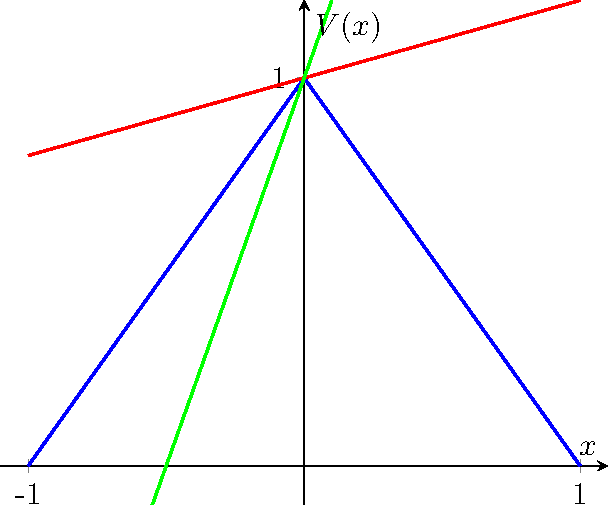
\includegraphics{Figs/tangent}
\caption{Red line is an acceptable tangent to the graph, while the green line is not. The green line does not keep the graph on one side locally.}
\label{fig:tangent}
\end{figure}
Therefore, we have $\varphi(t,x)=a\cdot (x-x_0)+b (t-t_0)+V(t_0,x_0)$ such that $\varphi(t,x)-f(t,x)$ has a local extrema at $(t_0,x_0)$.

For the second derivative tangent planes are not sufficient, because the second derivatives of the tangent planes are always zero. Therefore, we need to appeal to the quadratic functions of the form $\varphi(t,x)=(x-x_0)\cdot  A(x-x_0)+ a\cdot (x-x_0)+b (t-t_0)+ V(t_0,x_0)$. Note that since we have first derivative on $t$, we only use first order term on $t$. If a function $\varphi(t,x)$ touches $V(t,x)$ at point $(t_0,x_0)$ from above (resp. below), i.e., $(t_0,x_0)$ is a local minimum (maximum) point for $\varphi-V$, then we call $(b,a,A)=(\partial_t\varphi(t_0,x_0),\nabla\varphi(t_0,x_0),D^2\varphi(t_0,x_0))$ a superderivative (resp. sub) of $V$ at point $(t_0,x_0)$. Such functions $\varphi(t,x)$ are called test functions. See Figure~\ref{fig:viscosity}.

A function $\underline{V}$ (resp. $\overline{V}$) is called a viscosity subsolution (resp. super) of \eqref{eqn:nonlinear_parabolic} if for any superderivative (resp. sub) $(b,a,A)$ at point $(t_0,x_0)$, we have 
\begin{equation}
\begin{cases}		0\ge b+F\big(t_0,x_0,\varphi(t_0,x_0),a,A\big), ~~~~~\textrm{(resp. $0\le $)}\\
		V(T,x)\le g(x) ~~~~~\textrm{(resp. $0\ge $)}
\end{cases}
\end{equation}


\begin{figure}[ht!]
\centering
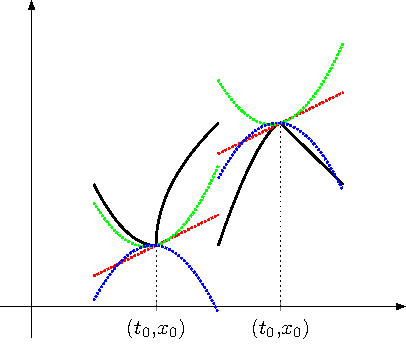
\includegraphics[width=0.8\textwidth]{Figs/viscosity}
\caption{The test functions that represent the sub and superderivatives of a function at the points of nondifferentiability as well as other points that the function is differentiable.}
\label{fig:viscosity}
\end{figure}
A function is called a viscosity solution if it is a sub and a super solution. 

\begin{rem}
The subsolution (resp. super) is named in accordance with submartingale (resp. super). If $U(t,x)\in\mathrm{C}^{1,2}$ is a subsolution (resp. super) to the equation 
\begin{equation}
		0=\partial_{t}V(t,x)+C(t,x)+\mu(t,x)\partial_{x}V(t,x)+\frac12{\sigma^2(t,x)}\partial_{xx}V(t,x),
\end{equation}
then $Y_t:=U(t,X_t)$ is a submartingale (resp. super) martingale, where
\begin{equation}
{\dX}_t=\mu(t,X_t){{\dt}}+\sigma(t,X_t){\dd}B_t.
\end{equation}
\end{rem}

For the first order HJB equation, finding the direction of the inequality for the subsolution or super solutions is not particularly obvious. It can be determined while we add a singular perturbation term $\eps B_t$ to the deterministic state process and send $\eps\to0$. For instance, in Exercise~\ref{ex:eikonal}, if we set the state process ${\dX}_t^u=u_t{{\dt}}+\eps {\dd}B_t$, we obtain the HJB 
\begin{equation}\label{eqn:Eikonal_perturbed}
\begin{cases}
		0=1-|V^{\prime}(x)|+\frac{\eps^2}{2}V^{\prime\prime}(x)\\
		V(\pm1)=0
\end{cases}
\end{equation}
In this case, the subsolution (resp. super) can satisfies
\begin{equation}
\begin{cases}
		0\ge1-|V^{\prime}(x)|+\frac{\eps^2}{2}V^{\prime\prime}(x)~~~~\textrm{(resp. $0\le$)}\\
		V(\pm1)\le0~~~~\textrm{(resp. $0\ge$)}
\end{cases}
\end{equation}
By sending $\eps\to0$, we obtain the following inequalities for the eikonal equation, \eqref{eqn:Eikonal_perturbed}.
\begin{equation}\label{eqn:Eikonal_sub_super}
\begin{cases}
		0\ge1-|V^{\prime}(x)|~~~~\textrm{(resp. $0\le$)}\\
		V(\pm1)\le0~~~~\textrm{(resp. $0\ge$)}
\end{cases}
\end{equation}
We can easily check that the function $V(t,x)=1-|x|$ is a viscosity solution of the eikonal equation, \eqref{eqn:Eikonal_perturbed}. For example, at all points $x\neq0$, the sub and superderivatives are equal to $-\textrm{sgn}(x)$, which obviously satisfy the equation with equality. At $x=0$, we only have super derivatives and the set of subderivatives is empty set. This makes the supersolution property to hold obviously by the false antecedent. The set of superderivatives contains all $m\in[-1,1]$. Since $0\le1-|m|$, then $V(t,x)=1-|x|$ is also a subsolution. All the above arguments are valid since the boundary condition $V(t,\pm1)=0$ validates the sub and supersolution properties. 

On the other hand, the function $\tilde{V}=\min\{|x|,1-|x|\}$ only satisfies the subsolution property. 
\begin{ex}
Show that $\tilde{V}$ is a viscosity subsolution to the eikonal equation \eqref{eqn:Eikonal_sub_super}, but not a super solution. Explore the points $x=\pm\frac12$.
\end{ex}

The existence and uniqueness of the solution to the nonlinear parabolic equations in the class of functions with linear growth is studies in several papers. For instance, see \cite{CIL92}. For the HJB equations derived from the optimal control problems, the value function of the control problem is usually the viscosity solution of the HJB. The uniqueness is due to a technical lemma, Ishii's lemma. However, in most cases, if we manage to show that any viscosity solution is indeed a classical solution, $\mathrm{C}^{1,2}$, then the verification theorem, Theorem~\ref{thm:verification} shows that any classical solution is equal to the value function, and therefore, uniqueness is obtained.


%%%%%%%%%%%%%%%%%%%%%%%%%%%%%%%%%%%%%%%%%%%%%%%%%%%%%%%%%%%%%%%%%%%%%

\section{Verification}\label{sec:verification}
Instead of going through viscosity solutions, we consider the cases where the HJB equation has a $C^{1,2}$ solution, which is a candidate for the value function. Then, we introduce a \emph{verification theorem}, which approves that the solution is indeed the value function.
\begin{thm}[Verification]\label{thm:verification}
    Let HJB equation, \eqref{eqn:HJB} has a $C^{1,2}$ solution, $v(t,x)$. Then, $v(t,x)\ge V(t,x)$.\\
In addition, assume that there exists $u^*(t,x)$ such that 
\begin{equation}
        u^*(t,x)\in\textrm{argmin}_{u}\Big\{C(t,x,u) +
         \frac12 D^2v(t,x) \cdot a(t,x,u) + \nabla v(t,x)\cdot \mu(t,x,u)\Big\}
\end{equation}
and $u^*(t,x)$ is an admissible Markovian (feedback) control, i.e., \eqref{eqn:state_Markov_control} has a (strong) solution, $X^*_t$, and $u^*_t=u^*(t, X^*_t)$ is admissible, $u^*\in\mathcal{A}$. Then, $v(t,x)=V(t,x)$.
\end{thm}
\begin{proof}
Since $v$ satisfies \eqref{eqn:HJB} in classical sense, we conclude that for any value of $u\in U$, we have 
\begin{equation}\label{eqn:subsol_thm_verif}
0\ge\partial_{t}v(t,x)+C(t,x,u)+\mu(t,x,u)\nabla v(t,x)+\frac12{a(t,x,u)}\cdot D^2v(t,x) 
\end{equation}
Since $v(t,x)\in\mathrm{C}^{1,2}$, it follows from the It\^o formula that for any $u\in\mathcal{A}_{t,T}$, 
\begin{equation}
\begin{split}
v&(T,X_T^{t,x,u})=v(t,x)\\
&+\int_0^T\Big(\partial_{t}v(s,X_s^{t,x,u})+\mu(s,X_s^{t,x,u},u_s)\cdot\nabla v(s,X_s^{t,x,u})+\frac12{a(s,X_s^{t,x,u},u_s)}\cdot D^2v(s,X_s^{t,x,u})\Big){{\ds}}\\
&+\int_t^T\sigma(s,X_s^{t,x,u},u_s){\dd}B_s
\end{split}
\end{equation}
By \eqref{eqn:subsol_thm_verif} and terminal condition $v(T,x)=g(x)$, we obtain
\begin{equation}\label{eqn:911}
g(X_T^u)\ge{v}(t,x)-\int_0^TC(s,X_s^{t,x,u},u_s){{\ds}}+\int_t^T\sigma(s,X_s^{t,x,u},u_s){\dd}B_s
\end{equation}
If we take conditional expectation, the martingale property of the stochastic integral implies that
\begin{equation}
\mathbb{E}_{t,x}\bigg[g(X_T^u)+\int_0^TC(s,X_s^{t,x,u},u_s){{\ds}}\bigg]\ge{v}(t,x)
\end{equation}
Now, by taking supremum over $u\in\mathcal{A}_{t,T}$, we obtain
\begin{equation}
V(t,x)=\sup_{u\in\mathcal{A}_{t,T}}\mathbb{E}_{t,x}\bigg[g(X_T^u)+\int_0^TC(s,X_s^{t,x,u},u_s){{\ds}}\bigg]\ge{v}(t,x).
\end{equation}\label{eqn:913}
Now, assume that  for some $u^*(t,X^*_t)\in\mathcal{A}$, $Y^{u^*}_t=v(t,X_t^{u^*})+\int_0^t C(s,X_s^{u^*},u^*_s) {{\ds}}$ is a martingale. By applying the It\^o formula, we have
\begin{equation}
\begin{split}
Y^{u^*}_t=&v(t,x)+\int_t^T\sigma(s,X_s^{t,x,u^*},u_s){\dd}B_s+\int_0^T\Big(\partial_{t}v(s,X_s^{t,x,u^*})+\mu(s,X_s^{t,x,u^*},u^*_s)\cdot \nabla v(s,X_s^{t,x,u^*})\\
&\hspace*{4cm}+\frac12{a(s,X_s^{t,x,u^*},u^*_s)}\cdot D^2v(s,X_s^{t,x,u^*})+C(s,X_s^{u^*},u^*_s)\Big){{\ds}}\\
=&v(t,x)+\int_t^T\sigma(s,X_s^{t,x,u^*},u_s){\dd}B_s
\end{split}
\end{equation}
Therefore, the martingale property of $Y^{u^*}$, implies that
\begin{equation}
\begin{split}
C(s,X_s^{u^*},u^*_s)+&\partial_{t}v(s,X_s^{t,x,u^*})+\mu(s,X_s^{t,x,u^*},u^*_s)\cdot\nabla v(s,X_s^{t,x,u^*})\\
+&\frac12{a(s,X_s^{t,x,u^*},u^*_s)}\cdot D^2v(s,X_s^{t,x,u^*})=0,~~~\textrm{a.s.}
\end{split}
\end{equation}
Therefore, for $u^*$, all the inequalities in \eqref{eqn:911}-\eqref{eqn:913} holds as equality and we obtain $v=V$.
\end{proof}
We apply Theorem~\eqref{thm:verification} to the following examples.
\begin{ex}
    [Merton optimal investment problem]{}
    Remember a self-financing portfolio with a 
    Black-Scholes risky asset, 
    ${{\dd}}S_t=S_t(\mu {{\dt}}+\sigma {\dd}B_t)$, 
    under zero interest rate  satisfies
    \begin{equation}
        {\dX}_t=\theta_t(\mu {{\dt}}+ \sigma {\dd}B_t)
    \end{equation}
    where $\theta$ is the amount of money invested in the risky asset.
    Merton problem is 
    \begin{equation}
        \sup_{\theta}\mathbb{E}[U(X_T^\theta)]
    \end{equation}
     The HJB is given by
     \begin{equation}
         \begin{cases}
             0=\partial_t v+ \sup_{\theta}\bigg\{\frac{\theta^2\sigma^2}{2}\partial^2_x v+\theta\mu \partial_x v\bigg\}\\
             v(T,x)=U(x)
         \end{cases}
     \end{equation}
     This simplifies to 
          \begin{equation}\label{eqn:HJB_merton_investment}
         \begin{cases}
             0=\partial_t v-\frac{(\mu \partial_x v)^2}{\sigma^2 \partial^2_x v}\\
             v(T,x)=U(x)
         \end{cases}
     \end{equation}
     For $U(x)=-e^{-\lambda x}$, with $\lambda>0$, use separation of variables $u(t,x)=-f(t)e^{-\lambda x}$ to find a closed form solution for the HJB.
\end{ex}
\begin{ex}
    For $U(x)=x^\lambda$, use separation of variables $u(t,x)=f(t)x^\lambda$ to find a closed form solution for the HJB. Is there any restriction on the value of $\lambda$?
\end{ex}
\begin{ex}
    For $U(x)=\ln x$, can you suggest a separation of variables?
\end{ex}

\begin{ex}
    [Merton optimal consumption problem]{}
    It is similar to the Merton optimal investment problem except, the investor is consuming from the account and what matters is the utility of consumption.
    \begin{equation}
        {\dX}_t=\theta_t(\mu {{\dt}}+ \sigma {\dd}B_t)-c_t{{\dt}}
    \end{equation}
    where $\theta$ is the amount of money invested in the risky asset and $c$ is the consumption with $c_t\ge0$.
    Merton problem is 
    \begin{equation}
        \sup_{\theta,c}\mathbb{E}\Big[\int_0^\infty e^{-\gamma t}U(c_t){\dt}\Big], ~\gamma>0
    \end{equation}
    Show that the HJB is given by
    \begin{equation}
        0= \sup_{\theta}\bigg\{\frac{\theta^2\sigma^2}{2}v^{\prime\prime}+\theta\mu v^\prime\bigg\}+\sup_{c\ge0}\Big\{U(c)-cv^\prime\Big\}-\gamma v
    \end{equation}
    or 
    \begin{equation}\label{eqn:HJB_consumption}
        0=\frac{(\mu v^\prime)^2}{\sigma^2 v^{\prime\prime}}+\sup_{c\ge0}\Big\{U(c)-cv^\prime\Big\}-\gamma v
    \end{equation}
For $U(c)=\frac{x^{1-\lambda}}{1-\lambda}$, with $\lambda\in(0,1)$, we have
\begin{equation}
    \sup_{c\ge0}\Big\{U(c)-cv^\prime\Big\}=U(c^*)-c^*v^\prime
\end{equation}
with $U^\prime(c^*)=v^\prime$ or $c^*$
\end{ex}

%%%%%%%%%%%%%%%
\subsection{Martingale approach}\label{sec:martingale}
The martingale principle for optimal control (\cite{DV73}) is another verification result which does not require the differentiability of the value function.
\begin{thm}\label{thm:martingale_verification}
	Assume that there exists a function $v(t,x)$ such that for all $u\in\mathcal{A}$ the process $\{Y^u_t\}_{t\ge0}$
	\begin{equation}
		Y^u_t:=v(t,X_t^u)+\int_0^tC(s,X_s^u,u_s){{\ds}}
	\end{equation}
	is a super martingale and that for some $u^*\in\mathcal{A}$, $\{Y^{u^*}_t\}_{t\ge0}$ is a martingale. Then, $u^*$ is an optimal control and the value function is equal to $v(t,x)$.
\end{thm}
\begin{proof}
By the supermartingale property, we have
\begin{equation}
Y^u_t\le\mathbb{E}[Y^u_T|\mathcal{F}_t]=\mathbb{E}\Big[g(X_T^u)+\int_t^TC(s,X_s^u,u_s){{\ds}}\Big|\mathcal{F}_t]\Big]+\int_0^tC(s,X_s^u,u_s){{\ds}}
\end{equation}
Thus, 
\begin{equation}
v(t,x)=Y^u_t-\int_0^tC(s,X_s^u,u_s){{\ds}}\le\mathbb{E}[Y^u_T|\mathcal{F}_t]=\mathbb{E}\Big[g(X_T^u)+\int_t^TC(s,X_s^u,u_s){{\ds}}\Big|\mathcal{F}_t]\Big],
\end{equation}
for all $u\in\mathcal{A}_{t,T}$. Given $X_t^u=x$, we obtain
\begin{equation}
v(t,x)\le\sup_{u\in\mathcal{A}_{t,T}}\mathbb{E}\Big[g(X_T^u)+\int_t^TC(s,X_s^u,u_s){{\ds}}\Big|X_t^u=x]\Big]=V(t,x).
\end{equation}
If for some $u^*$, $Y^{u^*}$ is a martingale, then in all the above, the inequality turns into equality and we have $v(t,x)=V(t,x)$.
%Since $V(t,x)\in\mathrm{C}^{1,2}$, we can apply It\^o formula to write 
%\begin{equation}
%\begin{split}
%Y^u_t=&\int_0^t\Big(C(s,X_s^u,u_s)+\partial_{t}V(s,X_s^u)+\mu(s,X_s^u,u_s)\partial_{x}V(s,X_s^u)+\frac{\sigma^2}{2}(s,X_s^u,u_s)\partial_{xx}V(s,X_s^u) \Big){{\ds}}\\
%&+\int_{t}^{\tau}\sigma(s,X_s^u,u_s)\partial_{x}V(s,X_s^u){\dd}B_t
%\end{split}
%\end{equation}
\end{proof}
The above theorem can also be regarded as a verification that a possible candidate $V(t,x)$ is a value function of the optimal control problem. The following example shows the use of this theorem.
\begin{eg}\label{eg:martingle_consumption}
In Example~\ref{eg:admissibility_paradox}, let $U(c)=\frac{c^{1-\alpha}}{1-\alpha}$ when $c\ge0$ and $-\infty$ otherwise. Consider the function $V(t,x)=e^{-\gamma (T-t)}(T-t+e^{A/\alpha t})^{\alpha}e^{-AT}U(x)$ with $A=r(1-\alpha)-\gamma+\frac{(\mu-r)(1-\alpha)}{2\sigma^2\alpha}$.
	\begin{equation}
		Y^u_t=V(t,X_t^u)+\int_0^te^{-\gamma s}U(c_s){{\ds}}.
	\end{equation}
	By It\^o formula, we have 
	\begin{equation}
	\begin{split}
				dY_t^u=&\Big(\partial_t V+ \big(\theta_t(\mu-r)+rX^u_t-c_t\big)\partial_x V+ 
\frac12\sigma^2\theta_t^2\partial_{xx} V+e^{-\gamma t}U(c_t)\Big){{\dt}}\\
		&+\sigma\theta_t\partial_x V {\dd}B_t. 
	\end{split}
	\end{equation}
	By direct calculation, one can see that 
	\begin{equation}
		\partial_t V+ \big(\theta_t(\mu-r)+rX^u_t-c_t\big)\partial_x V
		+\frac12\sigma^2\theta_t^2\partial_{xx} V+e^{-\gamma t}U(c_t)\le0,~~\mathbb{P}\textrm{-a.s.}
	\end{equation}
	for all values of  $\theta$ and $c$. In addition, for $c^*_t(x)=(\partial_x V(t,x))^{-1/\alpha}$ and $\theta^*_t(x)=-\frac{(\mu-r)\partial_xV(t,x)}{\sigma^2\partial_{xx}V(t,x)}$, 
	\begin{equation}
		\partial_t V+ \big(\theta_t(\mu-r)+rX^u_t-c_t\big)\partial_x V
		+\frac12\sigma^2\theta_t^2\partial_{xx} V+e^{-\gamma t}U(c_t)=0,~~\mathbb{P}\textrm{-a.s.}
	\end{equation}
It remains to show that $c^*$ and $\theta^*$ are admissible Markov controls, i.e., to show that 
	\begin{equation}
		dX^*_t=\Big(\theta_t(X^*_t)\big((\mu-r) {{\dt}}+\sigma {\dd}B_t\big)-rX^*_t{{\dt}}\Big)-c^*_t(X^*_t){{\dt}},
	\end{equation}
	has a strong solution. We leave the details as an exercise. 
\end{eg}
\begin{rem}\label{rem:inf_submartingale}
If the control problem is with infimum instead of supremum,
\begin{equation}
V(t,x)=\inf_{u\in\mathcal{A}_{t,T}}\mathbb{E}\left[\int_{t}^{T}C(s,X_s^{t,x,u},u_s){{\dt}}+g(X_T^{t,x,u})\right],
\end{equation}
Theorem~\ref{thm:martingale_verification} is should be modified. More precisely, $Y_t^u$ is a submartingale. 

For deterministic cases, supermartingale (resp. submartingale) means nonincreasing (resp. nondecreasing).
\end{rem}
Finding a candidate for a value function and an optimal control is the subject of the future sections.

%%%%%%%%%%%%%%%%%%%%
\section{Some nonstandard HJB equations}
In this section, we provide a review of some HJB equations that come from stochastic singular control, optimal stopping time, stochastic impulse control, and switching problems. The treatment of such problems via HJB equations is similar, however, we first need to derive HJB equations. 
\subsection{Stochastic singular control problems}
Consider the stochastic control problem below:
\begin{eg}
    \begin{equation}
        \inf_{u_t}\mathbb{E}\bigg[\int_0^T\Big(\frac12 X_t^2 - u_t\Big){\dt}+ X_T^2- X_T\bigg]
    \end{equation}
    with $u_t\ge0$ (takes nonnegative values) and 
    \begin{equation}
        {\dX}_t=(X_t+u_t){{\dt}}+\sigma {\dd}B_t
    \end{equation}
    The HJB  is formally written as 
    \begin{equation}
        \begin{cases}
            \partial_t V + x\partial_x V + \frac{\sigma^2}{2}\partial^2_{x} V + \frac12x^2 + \inf_{u\ge0} u(\partial_x V-1)=0\\
            V(T,x)=x^2-x
        \end{cases}
    \end{equation}
    Note that 
    \begin{equation}
        \inf_{u\ge0} u(\partial_x V-1)=
        \begin{cases}
            -\infty & \partial_x V-1<0\\
            0 & \partial_x V-1\ge0
        \end{cases}
    \end{equation}
    Therefore, it is natural to assume that the value function satisfies $\partial_x V-1\ge0$. In fact, we expect so find the value functions such that if $\partial_x V>1$, then $\partial_t V + x\partial_x V + \frac{\sigma^2}{2}\partial^2_{x} V + \frac12x^2=0$ and when $\partial_x V=1$, the we only have $\partial_t V + x\partial_x V + \frac{\sigma^2}{2}\partial^2_{x} V + \frac12x^2\le 0$. More precisely, inequality $\partial_x V-1\ge0$ divides $[0,T]\times\mathbb{R}$ into two regions: 
    \begin{itemize}
        \item $\mathbf{N} = \{(t,x): \partial_x V(t,x)>1\}$
        \item $\mathbf{R} = \{(t,x): \partial_x V(t,x)=1\}$
    \end{itemize}
Inside $\mathbf{N}$, we expect that $\partial_t V + x\partial_x V + \frac{\sigma^2}{2}\partial^2_{x} V + \frac12x^2=0$ holds. This equations has a solution of the form $v(t,x)=a(t)x^2+b(t)x+c(t)$. 

We denote the boundary of $\mathbf{N}$ by $\partial \mathbf{N}$ and we define $R(t)$ such that $(t,R(t))\in\partial\mathbf{N}$, assuming that $R(t)$ is uniquely determined.
In addition, we expect to see that the value function and its first derivative are the same in the both sides of $\partial \mathbf{N}$, particularly, $\partial_x V(t,R(t))=1$. Therefore, if $v$ is the solution to 
    \begin{equation}\label{eqn:for v in sigular example}
        \begin{cases}
            \partial_t v + x\partial_x v + \frac{\sigma^2}{2}\partial^2_{x} v + \frac12x^2 =0\\
            v(T,x)=x^2-x
        \end{cases}
    \end{equation}
    then, we anticipate to write 
    \begin{equation}
        V(t,x)=\begin{cases}
            v(t,x)& x\ge R(t)\\
            x-R(t)+v(t,R(t))& x< R(t)
        \end{cases}
    \end{equation}
Solving \eqref{eqn:for v in sigular example}, we obtain that $v(t,x)=\frac{5e^{2(T-t)}-1}{4}x^2-e^{T-t}x-\frac{\sigma^2}{4}\Big(T-t-\frac{5e^{2(T-t)}-1}{2}\Big)$ and, therefore, $R(t)=2\frac{e^{T-t}+1}{5e^{2(T-t)}-1}$. 
\end{eg}
\begin{ex}\label{ex:DS}
    \begin{equation}
        \inf_{u_t\ge0}\mathbb{E}\Big[\int_0^\tau e^{-r t} \Big(\mu - u_t\Big){\dt}\Big]
    \end{equation}
    where $\tau=\inf\{s\ge0: X_t=0\}$ with
    \begin{equation}
        {\dX}_t=(\gamma X_t-u_t){{\dt}}+\sigma {\dd}B_t, ~~ X_0=x\ge0
    \end{equation}
    Write the HJB and obtain the nonlinear term by evaluating the infimum. 
\end{ex}
Singular control problems are easy to detect; the running cost and drift of the SDE are both linear in the control. To see this, consider the control problem
\begin{equation}\label{eqn:dpp_singular}
        \inf_{u}\mathbb{E}\Big[\int_0^T \big(C(s,X^u_s)+au_s\big){{\ds}} + g(X_T^u)\Big]
    \end{equation}
where $u_t$ takes values in a closed convex cone $\mathcal{C}$ and 
\begin{equation}
	\begin{cases}
	    {\dX}^u_t =(\mu(t,X_t^u)+Au_t){{\dt}}+\sigma(t,X_t^u){\dd}B_t\\
     X^u_0=x\in\mathbb{R}^d
	\end{cases}
\end{equation}
The heuristic derivation of the HJB yields
\begin{equation}
    \begin{cases}
        0=\partial_t V(t,x)+\frac12  a(t,x,u)\cdot D^2V(t,x) +\nabla V(t,x)\cdot \mu(t,x)+C(t,x)+\inf_{u}\Big\{au +
           Au\cdot \nabla V(t,x)\Big\}\\
         V(T,x)=g(x)
    \end{cases}
\end{equation}
$a=\sigma^\intercal\sigma$. The infimum above is given by 
\begin{equation}
    \inf_{\hat{u}\in\mathcal{C},~|\hat{u}|=1,\lambda\ge0}\lambda \hat{u}\cdot \big(a +
          A\nabla V(t,x)\big)=\inf_{\lambda\ge0}\lambda \inf_{|\hat{u}|=1}\hat{u}\cdot \big(a +
          A\nabla V(t,x)\big)=\inf_{\lambda\ge0}\lambda \mathcal{H}(\nabla V(t,x))
\end{equation}
where $\mathcal{H}(\nabla V(t,x)):=\inf_{|\hat{u}|=1}\hat{u}\cdot \big(a +
          A\nabla V(t,x)\big)$. If $\mathcal{H}(\nabla V(t,x))<0$, then the infimum is $-\infty$ and the problem becomes degenerate. To avoid degeneracy, we must have $\mathcal{H}(\nabla V(t,x))\ge0$, in which case infimum is attained in $\lambda=0$ and we have 
\begin{equation}
    \begin{cases}
        0=\partial_t V(t,x)+\frac12  a(t,x,u)\cdot D^2V(t,x) +\nabla V(t,x)\cdot \mu(t,x)+C(t,x)\\
         V(T,x)=g(x)
    \end{cases}
\end{equation}
For simplicity of notation, we set
\begin{equation}\label{eqn:mathcalL}
   \mathcal{L}V(t,x):=\partial_t V(t,x)+\frac12  a(t,x,u)\cdot D^2V(t,x) +\nabla V(t,x)\cdot \mu(t,x)+C(t,x)
\end{equation}          

The interpretation of the HJB requires some \textit{variational inequalities}:\footnote{For more details on why we write the variational inequality this way, see \cite[Chapter 11]{Fleming-Soner-book-06} and the  notion of sub and super solutions.}
\begin{enumerate}
    \item for all $(t,x)$, $-\mathcal{L}V(t,x)\ge0$ and $\mathcal{H}\nabla V(t,x)\ge0$.
    \item If $\mathcal{H}(\nabla V(t,x))>0$, then $-\mathcal{L}V(t,x)=0$.
\end{enumerate}


The description of the optimal control in singular control problems need the notion of local time of SDEs. For instance, in Exercise~\ref{ex:DS}, the optimal control is the local time of the process, ${\dX}_t=\gamma X_t{{\dt}}+\sigma {\dd}B_t$ at the point $\hat{x}$, existence of which is obtained through solving the HJB and going through verification step. 
%%%%%%%%%%%%%%%%%%
\subsection{Optimal stopping problem}
Let $X$ be given by the SDE
\begin{equation}
    {\dX}_t = \mu(t,X_t){\dt}+\sigma(t,X_t){\dd}B_t
\end{equation}
in a filtered probability space
and consider the following problem
\begin{equation}
    \sup_{}\mathbb{E}\bigg[\int_0^{\tau\wedge T} e^{-rt} C(t,x_t){\dt} + g(X_{\tau\wedge T})\bigg]
\end{equation}
where the supremum is over all stopping time $\tau$ adapted to the filtration. These class of problems, which are not stochastic control problems,  called \emph{optimal stopping problems}. To solve optimal stopping problems, we can write the following DPP:
\begin{equation}
    V(t,x)=\mathbb{E}_{t,x}\bigg[\int_0^{\eta}e^{-r(s-t)}C(t,X_s){\ds}+e^{-r(\eta-t)}g(X_\eta)\bigg]
\end{equation}
for any stopping time $\eta$ with values in $[t,T]$. 
The DPP above leads to the following variational HJB equation:
\begin{enumerate}
    \item $V(t,x)\ge g(x)$ and $-\mathcal{L}V(t,x)\ge0$
    \item if $V(t,x)> g(x)$, then $-\mathcal{L}V(t,x)=0$
\end{enumerate}
where $\mathcal{L}$ is given in \eqref{eqn:mathcalL}.




%%%%%%%%%%%%%%%%%%%%%%%%%%%%%%%%%%%%%%%%%%%%%%%%%%%%%%%%%%%%%%%%%%%%
\section{Backward stochastic differential equations}
\label{sec:BSDE}
The backward stochastic differential equations (BSDE) is an alternative way to tackle the optimal control problems. One advantage of the BSDEs is that they can  cover the nonMarkovian optimal control problems. The derivation of the BSDEs from an optimal control problem follows from the It\^o martingale representation theorem. 
\begin{thm}
In a probability space which hosts a Brownian motion $B$, let $\mathbb{F}^B:=\{\mathcal{F}^B_t\}_t$ be the right-continuous augmented filtration generated by a Brownian motion $B$. 
Let $X$ be a $\mathcal{F}^B_T$-measurable random variable with finite expectation. Then, there exists a $\mathbb{F}^B$-progressively measurable process $Z_t(\omega)$ such that 
\begin{equation}
X=\mathbb{E}[X]+\int_0^TZ_t{\dd}B_t
\end{equation}

In addition, if $M$ is a continuous martingale with respect to $\mathbb{F}$, then, there exists a $\mathbb{F}^B$-progressively measurable process $\phi_(\omega)$ such that 
\begin{equation}
M_t=M_0+\int_0^tZ_s{\dd}B_s,~~~\textrm{for }~~~ t\ge0.
\end{equation}
\end{thm}
In the above theorem, $Z$ can interpreted as the sensitivity of the martingale $M$ with respect to the Browanian noise $B$.

Consider for a given stochastic process $C_t(\omega)$ 
\begin{equation}
Y_t:=\mathbb{E}\left[\int_t^T   L_s(\omega){{\ds}} + \xi \Big|\mathcal{F}^B_t\right].
\end{equation}
We simply assume that $r_s(\omega)$ and $L_s(\omega)$ are $\mathbb{F}^B$-progressively measurable processes and $\xi$ is a $\mathcal{F}_T^X$-measurable and integrable random variable. For the martingale define by 
\begin{equation}
M_t:=\mathbb{E}\left[\int_0^T  L_s(\omega){{\ds}}+\xi\Big|\mathcal{F}^B_t\right],
\end{equation}
and by the It\^o martingale representation theorem, we have
\begin{equation}
M_T=\int_0^T   L_s(\omega){{\ds}}+\xi=M_t+\int_t^TZ_s{\dd}B_s,
\end{equation}
for some $\mathbb{F}^B$-progressively measurable process $Z_t(\omega)$.
Since $Y_T=\xi$, we have 
\begin{equation}
M_T=\int_0^T   L_s(\omega){{\ds}}+Y_T=M_t+\int_t^TZ_s{\dd}B_s,
\end{equation}
On the other hand,
since $\int_0^t   L_s(\omega){{\ds}}$ is $\mathcal{F}^B_t$-measurable, we can write
\begin{equation}
M_t=\int_0^t   L_s(\omega){{\ds}}+\mathbb{E}\left[\int_t^T   L_s(\omega){{\ds}}+\xi\Big|\mathcal{F}^B_t\right]=\int_0^t   L_s(\omega){{\ds}}+Y_t.
\end{equation}
Therefore,
\begin{equation}
\int_0^T   L_s(\omega){{\ds}}+Y_T=\int_0^t   L_s(\omega){{\ds}}+Y_t+\int_t^TZ_s{\dd}B_s,
\end{equation}
or,
\begin{equation}\label{eqn:bsde_mg}
Y_t=Y_T+\int_t^T   L_s(\omega){{\ds}}-\int_t^TZ_s{\dd}B_s.
\end{equation}
The BSDE \eqref{eqn:bsde_mg} can be written formally by 
\begin{equation}
\begin{cases}
dY_t=- L(t,\omega){{\dt}}+Z_t{\dd}B_t\\
Y_T=g(X_T)
\end{cases}
\end{equation}
Note that we could have written the above forwardly, i.e.,
$Y_t=Y_0+\int_0^t   L_s(\omega){{\ds}}-\int_0^tZ_s{\dd}B_s$. However, this is not very useful, because $Y_0$ is not known. See example below.
\begin{eg}
Recall that
the solution to the linear equation 
\begin{equation}
\begin{cases}
		0 =\partial_{t}v(t,x)+C(t,x)+[\mu \cdot\nabla v](t,x)+\frac12[\sigma^\intercal\sigma \cdot D^2v](t,x)\\
v(T,x)=g(x)
\end{cases}		
\end{equation}
is given by the Feynmann-Kac formula:
\begin{equation}
V(t,x)=\mathbb{E}\left[\int_t^T C(s,X_s){{\ds}}+g(X_T)\Big| X_t=x\right],
\end{equation}
where
\begin{equation}
{\dX}_t=\mu(t,X_t){{\dt}}+\sigma(t,X_t){\dd}B_t.
\end{equation}
If we define $Y_t=V(t,X_t)$, then \eqref{eqn:bsde_mg} is given by 
\begin{equation}
Y_t=g(X_T)+\int_t^T C(s,X_s){{\ds}}-\int_t^TZ_s{\dd}B_s.
\end{equation}
In the above, $g$ and $L$ are known. Given that we can find $Z$, $Y_t$ is known. However, if we write the equation forward
\begin{equation}
Y_t=Y_0+\int_0^t C(s,X_s){{\ds}}-\int_0^tZ_s{\dd}B_s.
\end{equation}
Here, $Y_0=V(0,X_0)$ is not known. 
\end{eg}


The following theorem shows that a BSDE can generalize the Feynmann-Kac formula to nonlinear equations.
\begin{thm}\label{thm:Markov_BSDE}
Assume that the following \emph{semilinear}\footnote{The an equation with linear second order term and possibly nonlinear first order term is called semilinear.} PDE has a solution $V(t,x)\in\mathrm{C}^{1,2}$.
\begin{equation}\label{eqn:semilinear_PDE}
\begin{cases}
0=\partial_{t}v(t,x)+[\mu\cdot{\nabla}v](t,x)+\frac12[{\sigma^\intercal\sigma\cdot}D^2V](t,x)+C(t,x,v(t,x),\nabla v(t,x))\\
V(T,x)=g(x).
\end{cases}		
\end{equation}
Then, $Y_t=V(t,X_t)$ and  $Z_t=\sigma(t,X_t)\nabla V(t,X_t)$ satisfy the BSDE
\begin{equation}\label{eqn:Markov_BSDE}
\begin{cases}
dY_t=- C(t,X_t,Y_t,\sigma^{-1}(t,X_t)Z_t){{\dt}}+Z_t{\dd}B_t\\
Y_T=g(X_T)
\end{cases}
\end{equation}
where 
\begin{equation}
{\dX}_t=\mu(t,X_t){{\dt}}+\sigma(t,X_t){\dd}B_t.
\end{equation}
\end{thm}
\begin{proof}
By applying It\^o lemma on $Y_t=V(t,X_t)$, we obtain
\begin{equation}
\begin{split}
dY_t=&\big(\partial_{t}V(t,X_t)+\mu(t,X_t)\nabla V(t,X_t)+\frac12{\sigma^2(t,X_t)}\partial_{xx}V(t,X_t)\big){{\dt}}+\sigma(t,X_t)\nabla V(t,X_t){\dd}B_t\\
&=-C(t,X_t,V(t,X_t),\nabla V(t,X_t)){{\dt}}+\sigma(t,X_t)\nabla V(t,X_t){\dd}B_t\\
&=- C(t,X_t,Y_t,\sigma^{-1}(t,X_t)Z_t){{\dt}}+Z_t{\dd}B_t
\end{split}
\end{equation}
\end{proof}

In the above, the second equality is obtained from the PDE and the third equality is from the definition of $Y$ and $Z$. In addition, by the terminal condition we have, $Y_T=V(T,X_T)=g(X_T)$.
In general, the use of BSDEs over the HJB is  preferable when the regularity of the function $V(t,x)$ is not established. Because by the existence theorem for the BSDEs, we already know that  $Z_t$ exists as stochastic process even if $\sigma(t,X_t)\nabla V(t,X_t)$ does not make sense in cases when $\nabla V$ does not exist as specific points.

Motivated by Theorem~\ref{thm:Markov_BSDE}, we can define a general BSDE as 
\begin{equation}\label{eqn:BSDE}
	\begin{cases}
		dY_t=-C(t,Y_t,Z_t,\omega){{\dt}}+Z_s{\dd}B_s\\
		Y_T=\xi
	\end{cases},
\end{equation}
The argument $\omega$ inside $L$ represents a general dependence on the randomness. In particular, it can represent solution $X_t$ of a possible path-dependent SDE
\begin{equation}
	{\dX}_t=\mu(t,X_\cdot){{\dt}}+\sigma(t,X_\cdot){\dd}B_t,
\end{equation}   
a possible control process $u_t$, or both $X_t$ and $u_t$. We discuss such dependencies in further details in Section~\ref{sec:max_principle}.
\begin{rem}
	In \eqref{eqn:BSDE}, we blended $\sigma^{-1}$ inside the Lagrangian $L(s,X_s,Y_s,\sigma^{-1}Z_s,\omega)$  into it and simply write $L(s,X_s,Y_s,Z_s,\omega)$.
\end{rem}
\begin{thm}[Existence and uniqueness theorem for BSDEs]
Assume that 
\begin{enumerate}[label=\bfseries \roman*)]
\item $\mu(t,x)$ and $\sigma(t,x)$ are Lipschitz in $t$ and $x$
\item for all $(t,x)$ with $0<\lambda|x|^2\le x^{\top}\sigma^{\top}\sigma x$ for all $x$ and  for some $\lambda$ (in particular $\sigma$ is invertible)
\item $L(t,x,\varrho,\Pi,\omega)$ is progressively measurable in $\omega$ and Lipschitz in  other variables $(t,x,\varrho,\Pi)$ and is decreasing in $\varrho$ a.s.
\end{enumerate} 
Then, for any $\mathcal{F}_T$-measurable square-integrable random variable $\xi$, there exists a couple $(Y_t,Z_t)$ such that \eqref{eqn:BSDE} holds, i.e.,
\begin{equation}
Y_t=\xi+\int_t^TL(s,X_s,Y_s,Z_s,\omega){{\ds}}-Z_s{\dd}B_s,
\end{equation}
and there exists a constant $C$ that only depends on the Lipschitz constant of $\mu$, $\sigma$, and  $L$ and the constant $\lambda$ that
\begin{equation}
\mathbb{E}\left[\sup_{t\in[0,T]}|Y_t|^2+\int_0^TZ_s^2{{\ds}}\right]\le C\left(\mathbb{E}[\xi^2]\right)
\end{equation}
\end{thm}


\subsection{Linear BSDEs}
Linear BSDEs take the form
\begin{equation}\label{eqn:linear_BSDE}
dY_t=-(\alpha_tY_t+\beta_tZ_t+L_t){{\dt}}+Z_t{\dd}B_t,
\end{equation}
where $\alpha$, $\beta$, and $L$ are arbitrary progressively measurable processes.
One can write a closed-form solution for a linear BSDE. To do so, note that
\begin{equation}
	dY_t=-(\alpha_tY_t+L_t){{\dt}}+Z_tdB^{\beta}_t,
\end{equation}
where by the Girsanov theorem, $dB^{\beta}_t:=\beta_t{{\dt}}+{\dd}B_t$ is a Brownian motion under the probability $\mathbb{P}^{\beta}$ given in
\begin{equation}
	\frac{d\mathbb{P}^{\beta}}{d\mathbb{P}~}\Big|_{\mathcal{F}_t}:=\exp\left(
	\int_0^t\beta_s {\dd}B_s-\frac12\int_0^t\beta^2_s{{\ds}}
	\right)
\end{equation}
If we define $\tilde{Y}_t:=e^{\int_0^t \alpha_s{{\ds}}}Y_t$, then
\begin{equation}
	d\tilde{Y}_t=e^{\int_0^t \alpha_s {{\ds}}}\left(L_t{{\dt}}+Z_tdB^{\beta}_t\right).
\end{equation}
In other words,
\begin{equation}
	\tilde{Y}_t=\tilde{Y}_T-\int_{t}^{T} e^{\int_0^s \alpha_z dz}\left(L_s{{\dt}}+Z_sdB^{\beta}_s\right),
\end{equation}
or, 
\begin{equation}
	{Y}_t=e^{\int_t^T \alpha_s{{\ds}}}\tilde{Y}_T-\int_{t}^{T} e^{\int_t^s \alpha_z dz}\left(L_s{{\dt}}+Z_sdB^{\beta}_s\right)=e^{\int_t^T \alpha_s{{\ds}}}\xi-\int_{t}^{T} e^{\int_t^s \alpha_z dz}\left(L_s{{\dt}}+Z_sdB^{\beta}_s\right).
\end{equation}
After taking conditional expectation with respect to $\mathbb{P}^{\beta}$, we obtain
\begin{equation}
	Y_t=\mathbb{E}^{\beta}\left[e^{\int_t^T \alpha_s {{\ds}}}\xi-\int_{t}^{T} e^{\int_t^s \alpha_z dz}L_s{{\dt}}
	\Big|\mathcal{F}_t\right].
\end{equation}
If we define 
\begin{equation}
	\Gamma_t=e^{\int_t^T \alpha_s {{\ds}}}\frac{d\mathbb{P}^{\beta}}{d\mathbb{P}~}\Big|_{\mathcal{F}_t}=\exp\left(
	\int_0^t\beta_s {\dd}B_s+\int_0^t(\alpha_s-\frac12\beta^2_s){{\ds}}
	\right),
\end{equation}
by changing the measure back to $\mathbb{P}$
\begin{equation}
	Y_t=\Gamma^{-1}_t\mathbb{E}\left[\Gamma_{T} \xi-\int_{t}^{T} \Gamma_{s} L_s{{\dt}}
	\Big|\mathcal{F}_t\right].
\end{equation}

%%%%%%%%%%%%%%%%%%%%%%%%%%%%%%%%%%%%%%%%%%%
\subsection{Comparison principle}\label{sec:comp_principle}
Consider 
\begin{equation}\label{eqn:comp_principle}
	\begin{cases}
		dY^{(i)}_t=-L^{(i)}(t,Y^{(i)}_t,Z^{(i)}_t,\omega){{\dt}}+Z^{(i)}_s{\dd}B_s\\
		Y^{(i)}_T=\xi^{(i)}
	\end{cases},
\end{equation}
for $i=1,~2$. The following theorem provides a sufficient condition for comparing $Y^{(1)}$ and $Y^{(2)}$, and hence, it is called comparison principle.
\begin{thm}\label{thm:comp_principle}
Assume that for $i=1,~2$, $(Y^{(i)},Z^{(i)})$ is the solution for \eqref{eqn:comp_principle} and $L(t,y,z,\omega)$ is Lipschitz in $(y,z)$ uniformly in $\omega$ and $t$.
	Further assume that $\xi^{(1)}\ge\xi^{(2)}$ and, for each value $(t,y,z)$, $L^{(1)}(t,y,z,\omega)\le L^{(2)}(t,y,z,\omega)$, a.s.
	Then, $Y^{(1)}\ge Y^{(2)}$, a.s.
\end{thm}
\begin{proof}
	
\end{proof}

%%%%%%%%%%%%%%%%%%%%%%%%%%%%%%%%%%%%%%%%%%%
\subsection{Maximum principle}\label{sec:max_principle}
For the purpose of control theory, we assume that $L$ takes the form $L(t,x,\varrho,\Pi,u_t)$, where $u_t$ is a progressively measurable process that represents a control at time $t$.
In this case, we denote the solution to the BSDE by $(Y^u,Z^u)$, where  
\begin{equation}
\begin{cases}
Y^u_t=\xi+\int_t^TF(s,X_s,Y^u_s,Z^u_s,u_s){{\ds}}-\int_t^TZ^u_s{\dd}B_s\\
%dY^u_t=-F(t,X_t, Y^u_t, Z^u_t, U_t){{\dt}}+Z^u_t {\dd}B_t\\
Y_T=\xi\in\mathcal{F}^{X}_t\\
{\dX}_t=\mu(t,X_t){{\dt}}+\sigma(t,X_t){\dd}B_t
\end{cases}
\end{equation}
and $F(s,X^u_s,Y^u_s,Z^u_s,u_s)=L(s,X_s,Y_s,\sigma^{-1}(s,X^u_s,u_s)Z_s,u_s)$.
Then, a control problem can be written as 
\begin{equation}
Y_t=\mathrm{esssup}_{u\in\mathcal{A}_{t,T}}Y_t^u.
\end{equation}
Note that the set of admissible controls are defined specific to a particular problem. In addition, if the terminal condition $\xi=g(X_t^u)$, the problem is a Markovian control problem that was studied in previous sections. Otherwise, it is not Markovian, and therefore, the value  cannot be written as a function $V(t,x)$. In fact, value function takes a more general form of 
\begin{equation}
Y_t=\mathrm{esssup}_{u\in\mathcal{A}_{t,T}}\mathbb{E}\left[\int_t^TF(s,X^u_s,Y^u_s,Z^u_s,u_s){{\ds}}+\xi\Big|\mathcal{F}^X_t\right].
\end{equation}
In the above, the Lagrangian $F$ not only depends on the state of the system $X_s^u$ and control $u_s$, but also depends on the history of the value $Y^u_s$ and the sensitivity of the value with respect to the Brownian noise $Z^u_t$.


To solve such optimal control problems, we require the following comparison principle.

\begin{thm}[Maximum principle for BSDEs]
The process 
\begin{equation}
Y_t=\mathrm{esssup}_{u\in\mathcal{A}_{t,T}}\mathbb{E}\left[\int_t^TF(s,X^u_s,Y^u_s,Z^u_s,u_s){{\ds}}+\xi\Big|\mathcal{F}^X_t\right]=\mathrm{esssup}_{u\in\mathcal{A}_{t,T}}Y_t^u
\end{equation}
there exists a $Z$ such that $(Y,Z)$
satisfies the BSDE
\begin{equation}
\begin{cases}
Y_t=\xi+\int_t^TF^*(s,X_s,Y_s,Z_s){{\ds}}-\int_t^TZ_s{\dd}B_s\\
Y_T=\xi\in\mathcal{F}^{X}_T\\
{\dX}_t=\mu(t,X_t){{\dt}}+\sigma(t,X_t){\dd}B_t
\end{cases}
\end{equation}
where
\begin{equation}
F^*(s,x,y,z):=\sup_{u\in U}F(t,x,y,z,u),~~~\textrm{and}~~~u^*(t,x,y,z):=\mathrm{argmax}_{u\in U}F(t,x,y,z,u)
\end{equation}
\end{thm}
%%%%%%%%%%%%%%%%
%%%%%%%%%%%%%%%%
%%%%%%%%%%%%%%%%
\chapter{Numerical evaluation of stochastic control problems}



%%%%%%%%%%%%%%%%
\section{DPP based approximation}
Recall from \eqref{eqn:dpp_discrete}, the value function and the optimal control in discrete stochastic control problem \eqref{prob:discrete_optimal_control} can be evaluated through.
\begin{equation}\label{eqn:dpp_discrete_numerical}
    \begin{cases}
        V(t,x)= \inf_{u}
    C(t,x,u) + \mathbb{E}[V(t+1,X^u_{t+1})|X_t=x]\\
    V(T,x)=g(x)\\
    u^*_t(x)\in A(x):=\textrm{argmax}_{u}
    C(t,x,u) + \mathbb{E}[V(t+1,X^u_{t+1})|X_t=x]
    \end{cases}
\end{equation}
where
\begin{equation}
    X^u_{t+1}=x+\mu(t,x,u)+\sigma(t,x,u)\xi_{t+1}
\end{equation}
and $\{\xi_t\}_{t=1}^T$ is a sequence of i.i.d. random variables with mean $0$ and variance $1$. In the above, we need to evaluate (1) conditional expectation $\mathbb{E}[\cdot|X_t=x]$ and (2) the infimum over control $u$. Given $V(t+1,\cdot)$, these calculations can be done separately. However, the separate evaluation creates inefficiency in the calculations. Therefore, we propose the one-shot approximation of $\inf_{u}C(t,x,u) + \mathbb{E}[V(t+1,X^u_{t+1})|X_t=x]$ through the following methods. 

\subsection{Evaluation of infimum}
First note that 
\begin{equation}
\begin{split}
    C(t,x,u(x))+&\mathbb{E}[V(t+1,X^u_{t+1})|X_t=x]
    \\
    &=\mathbb{E}[C(t,X,u(X))+ V(t+1,X+\mu(t,X,u(X))+\sigma(t,X,u(X))\xi_{t+1})|X=x]
\end{split}
\end{equation}
Denoting the right-hand side above by $\Phi(x,u)$, then we seek a function $\hat{u}^*(x)$ such that 
\begin{equation}\label{eqn:hatu^*}
    \hat{u}^*(\cdot)\in A(X):=\textrm{argmin}_{u(\cdot)}\mathbb{E}[\Phi(X,u(X))]
\end{equation}
The following Lemma guarantees that $\hat{u}^*$ solves \eqref{eqn:dpp_discrete_numerical}.
\begin{lem}\label{lem:expectation_minimization}
    Assume that $\hat{u}^*\in A(X)$ defined above. Then, $\hat{u}^*(x)\in A(x)$ for all $x$ in the set of values of $X$.
\end{lem}
\begin{proof}
     For a complete proof, we need a measurable selection theorem and some other conditions. For simplicity, we only provide the sketch of the proof. Assume that $u^*(x)\not\in A(x)$ with a positive probability on the set of values of $X$. We denote the set by $B$. Then, $x\in B$, we define $\tilde{u}^*(x)$ such that
     \[
     \tilde{u}^*(x)\in\textrm{argmax}_{u}
    C(t,x,u) + \mathbb{E}[V(t+1,X^u_{t+1})|X_t=x]
     \]
     and $\tilde{u}^*(x)=\hat{u}^*(x)$. 
     Therefore, 
     \[
     \mathbb{E}[\Phi(X,\tilde{u}^*(X))]<\mathbb{E}[\Phi(X,\hat{u}^*(X))]
     \]
     which contradicts the definition of $\hat{u}^*$.
\end{proof}

From the nonparametric point of view, we can approximate $\hat{u}^*(\cdot)$ in \eqref{eqn:hatu^*} by a nonparametric model $u(\cdot;\theta)$ via the following optimization
\begin{equation}
    \theta^*\in \textrm{argmin}_{\theta}\mathbb{E}[\Phi(X,u(X;\theta))]
\end{equation}
For instance, $u(\cdot;\theta)$ can be a neural network with parameter $\theta$.

\section{Multi-step evaluation}
While \eqref{eqn:dpp_discrete_numerical} is a classic way to evaluate optimal control problems, it is not very efficient. There are two reasons for the lack of efficiency. First, we have to run a loop over the number of time steps. Second, after evaluation of each nonparametric, we need to evaluate the value function. The total number of parameters is the number of parameters in each step times the number of steps, which for nonparametric models is massive and  potentially needs a lot of memory. Therefore, we propose the following optimization in place of \eqref{eqn:dpp_discrete_numerical}.
\begin{equation}
     \inf_{u(\cdot,\cdot)} \mathbb{E}\bigg[\sum_{t=0}^{T-1}C(t,X^u_t,u(t,X^u_t))+g(X^u_T)\bigg]
\end{equation}
where
\begin{equation}
\begin{cases}
        X^u_{t+1} =X^u_{t}+\mu(t,X^u_{t},u(t,X^u_{t}))+\sigma(t,X^u_{t},u(t,X^u_{t}))\xi_{t+1}\\
        X_0\textrm{ is a random variable.}
\end{cases}
\end{equation}
The justification for the above problem is the same as Lemma~\ref{lem:expectation_minimization} for one-step DPP method. 
Note that we can use a nonparametric model, $u(t,x;\theta)$,  to approximate the minimization problem by
\begin{equation}
\theta^*\in \textrm{argmin}_{\theta}\mathbb{E}\bigg[\sum_{t=0}^{T-1}C(t,X^u_t,u(t,X^u_t;\theta))+g(X^u_T)\bigg]
\end{equation}
with 
\begin{equation}
\begin{cases}
        X^u_{t+1} =X^u_{t}+\mu(t,X^u_{t},u(t,X^u_{t};\theta))+\sigma(t,X^u_{t},u(t,X^u_{t};\theta))\xi_{t+1}\\
        X_0\textrm{ is a random variable.}
\end{cases}
\end{equation}
When an approximate optimal strategy, $u(t,x;\theta^*)$, is found, then one can find the value function through evaluating 
\begin{equation}
    \mathbb{E}_{t,x}\bigg[\sum_{s=t}^{T-1}C(s,X^u_s,u(t,X^u_s;\theta^*))+g(X^u_T)\bigg]
\end{equation}
with
\begin{equation}
\begin{cases}
        X^u_{s+1} =X^u_{s}+\mu(s,X^u_{s},u(s,X^u_{s};\theta^*))+\sigma(s,X^u_{s},u(s,X^u_{s};\theta^*))\xi_{s+1}\\
        X_t=x
\end{cases}
\end{equation}
Of course, the evaluation of the conditional expectation above is a different problem.



% {\color{red}
% After finding or approximating }$\hat\phi(t,x,u)\approx$, we need to evaluate 
% \begin{equation}
%     u^*(x):=\inf_{u(x)} C(t,x,u(x)) + \hat\phi(t,x,u(x))
% \end{equation}
% To find such a function, one can solve the following risk minimization:
% \begin{equation}
%     \inf_{u(t,x)}\mathbb{E}[C(t,X,u(X)) + \hat\phi(t,X,u(X))]
% \end{equation}
% or empirically:
% \begin{equation}
%     \hat{u}(t,x)\in\argmin_{u(x;\theta)}J^{-1}\sum_{j\in[J]}C(t,X^j,u(X^j;\theta)) + \hat\phi(t,X^j,u(X^j;\theta))]
% \end{equation}
% Then, 
% \begin{equation}
%     \hat{V}(t,x)= 
%     C(t,x,\hat{u}(t,x)) + \hat\phi(t,x,\hat{u}(t,x)]
% \end{equation}
% One-step dynamic programming principle is laid out in Figure~\ref{fig:one-step}
% \begin{figure}
%     \centering
%     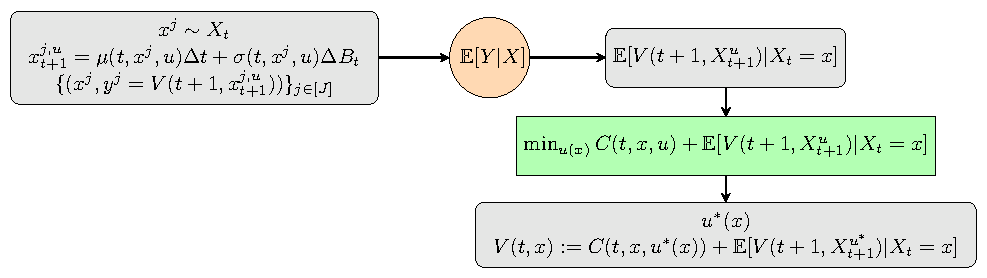
\includegraphics{Figs/one_step_DPP_chart.pdf}
%     % 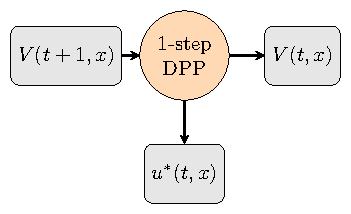
\includegraphics{Figs/one_step_DPP_chart_2.pdf}
%     \caption{One-step dynamic programming principle}
%     \label{fig:one-step}
% \end{figure}


% \begin{rem}
%     The challenges of evaluation of conditional expectation and evaluation of value function, makes implementation of the one-step DPP impractical. We are better off if we only use DPP for theoretical implications and do numerical implementations in different ways. However, in most methods we require the evaluation of conditional expectation.
% \end{rem} 


% %%%%%%%%
% \subsection{Evaluation of conditional expectation}
% We require to evaluate $\mathbb{E}[V(t+1,X^u_{t+1})|X_t=x]$  before the infimum in \eqref{eqn:dpp_discrete}. We first write $\phi(t,x,u):=\mathbb{E}[V(t+1,X^u_{t+1})|X_t=x]$, where $\phi(t,X^u_t,u)=\mathbb{E}[V(t+1,X^u_{t+1})|X_t]$. By the definition of conditional expectation,
% \begin{equation}
%     \phi(t,X_t,u)=\argmin_{\psi(x)}\mathbb{E}[(V(t+1,X^u_{t+1})-\psi(X_t))^2].
% \end{equation}
% Choosing a parametric or non-parametric model for $\psi$ leads to approximation:
% \begin{equation}
%     \hat\phi(t,X_t,u)=\argmin_{\theta}\mathbb{E}[(V(t+1,X^u_{t+1})-\psi(X_t;\theta))^2]
% \end{equation}
% Note that we can choose to generate samples for $X_t$ according to an arbitrary distribution and use \eqref{eqn:discrete_state} to simulate joint samples of $(X_t,X^u_{t+1})$. Then, the above approximation of conditional expectation will be performed empirically by 
% \begin{equation}
%     \hat\phi(t,X_t,u) \approx\argmin_{\theta}J^{-1}\sum_{j\in[J]}[(V(t+1,X^{u,j}_{t+1})-\psi(X^{j}_t;\theta))^2
% \end{equation}

\section{Numerical methods based on BSDEs}
Recall from Section~\ref{sec:BSDE} that the solution $V(t,x)$ to the semilinear equation 
\begin{equation}
\begin{cases}
0=\partial_{t}v(t,x)+[\mu\cdot{\nabla}v](t,x)+\frac12[{\sigma^\intercal\sigma\cdot}D^2V](t,x)+C(t,x,v(t,x),\nabla v(t,x))\\
V(T,x)=g(x).
\end{cases}		
\end{equation}
is related to the BSDE
\begin{equation}
\begin{cases}
dY_t=- C(t,X_t,Y_t,\sigma^{-1}(t,X_t)Z_t){{\dt}}+Z_t{\dd}B_t\\
Y_T=g(X_T)
\end{cases}
\end{equation}
by 
\begin{equation}
    Y_t=V(t,X_t) \textrm{ and } Z_t=[\sigma\nabla V](t,X_t)
\end{equation}
where 
\begin{equation}\label{eqn:sde_YZ}
{\dX}_t=\mu(t,X_t){{\dt}}+\sigma(t,X_t){\dd}B_t.
\end{equation}
One way to interpret the solution to the PDE is to find  functions $\mathbf{Y}(t,x)$ and $\mathbf{Z}(t,x)$ such that 
\begin{equation}\label{eqn:BSDE_YZ}
\mathbf{Y}(t,X_t)=g(X_T) -\int_t^T \Big(C(s,X_s,\mathbf{Y}(s,X_s),\mathbf{Z}(s,X_s)){{\ds}}+\mathbf{Z}(s,X_s){\dd}B_s\Big)
\end{equation}
Functions $\mathbf{Y}$ and $\mathbf{Z}$ can be approximated by neural networks $\hat{\mathbf{Y}}(t,x,\alpha)$ and $\hat{\mathbf{Z}}(t,x;\beta)$ and the equations \eqref{eqn:sde_YZ} and \eqref{eqn:BSDE_YZ} can be approximated discretely by 
\begin{equation}
\begin{cases}
\hat{\mathbf{Y}}(t_n,\hat{X}_{t_n})
=\hat{\mathbf{Y}} (t_{n+1},\hat{X}_{t_{n+1}}) 
- C(t_n,\hat{X}_{t_n},\hat{\mathbf{Y}}(t_n,\hat{X}_{t_n}),\hat{\mathbf{Z}}(t_n,\hat{X}_{t_n})) \Delta t
+\hat{\mathbf{Z}}(t_n,\hat{X}_{t_n})\Delta B_{t_{n+1}}\\
\hat{X}_{t_{n+1}}=\hat{X}_{t_n}+\mu(t_n,\hat{X}_{t_n})\Delta t+\sigma(t_n,\hat{X}_{t_n})\Delta B_{t_{n+1}}.
\end{cases}
\end{equation}
Specifically, we shall determine $\hat{\mathbf{Y}}$ and $\hat{\mathbf{Z}}$ such that $g(\hat{X}_T)$ is as close to $\hat{\mathbf{Y}}(T,\hat{X}_T)$ as possible. In other words,  we can find the approximate solution $\hat{\mathbf{Y}}(t,x,\alpha^*)$ and $\hat{\mathbf{Z}}(t,x;\beta^*)$ with 
\begin{equation}
    (\alpha^*,\beta^*)\in\mathop\textrm{argmin}\limits_{\alpha,\beta}\mathbb{E}\Big[\big(\hat{\mathbf{Y}}(T,\hat{X}_T)-g(\hat{X}_T)\big)^2\Big]
\end{equation}

\appendix
%%%%%%%%%%%%%%%%%%%%%%%%%%%%%%%
%%%%%%%%%%%%%%%%%%%%%%%%%%%%%%%
%%%%%%%%%%%%%%%%%%%%%%%%%%%%%%%
\section{Results from optimization}
In this sections, we quickly review two of the most influential results from optimization, namely the Lagrange multiplier and gradient descent, which later be used in the context of control problems. 
%%%%%%%%%%%%%%%%%%%%%%%%%%%%%%%
\subsection{Lagrange multiplier}
If we add a constraint to a simple minimization problem such as $\min_x f(x)$, the Lagrange multiplier method is the way to proceed. In a nutshell, the Lagrange multiplier method turns a constrained optimization problem into a saddle point problem without constraints by adding more variables. 

Consider  the constrained problem below:
\begin{equation}        
\label{constraint_optimization1}
    \inf_x f(x) ~~~ \textrm{subject to}~~~g(x)=0
\end{equation}
Define the Lagrangian:
\begin{equation}\label{lagrangian}
    L(x,\lambda):= f(x) - \lambda \cdot g(x)
\end{equation}
Then, under proper conditions, the following saddle point problem yields the solution to \eqref{constraint_optimization1}.
\begin{equation}
\sup_{\lambda}\inf_{x}L(x,\lambda)
\end{equation}
The function $H(\lambda)=\inf_{x}L(x,\lambda)$ is called Hamiltonian and the Lagrange multiplier $\lambda$ is called the dual variable. The unconstrained problem
\begin{equation}\label{prob:dual}
    \sup_{\lambda}H(\lambda)
\end{equation}
is called the \emph{dual problem} for the \emph{primal problem} \eqref{constraint_optimization1}.

The key to the success of the Lagrange multiplier method is the \emph{strong duality}.
\begin{equation}
    \sup_{\lambda}\inf_{x} L(x,\lambda)=\inf_{x}\sup_{\lambda}L(x,\lambda)
\end{equation}
With strong duality, if for some $x$, $g(x)\neq(0)$, then 
\begin{equation}
    \sup_{\lambda}L(x,\lambda) = \sup_{\lambda}\{f(x) - \lambda \cdot g(x)\} = \infty
\end{equation}
Therefore, $\inf_{x}\sup_{\lambda}L(x,\lambda)$ is restricted to $x$ with $g(x)=0$ and 
\begin{equation}
    \inf_{x:g(x)=0} \sup_{\lambda}L(x,\lambda) = \inf_{x:g(x)=0} f(x)
\end{equation}

It is not always easy to check if strong duality holds. 
However, \emph{Karush-Kuhn-Tucker} conditions (KKT) provide some necessary and sufficient conditions for strong duality.
\begin{thm}
Assume the differentiability of $f$ and $g$.
    If $x^*$ solves \eqref{constraint_optimization1}  and $\lambda^*$ solves \eqref{prob:dual} such that 
    \begin{equation} \label{cond:KKT}
    \begin{cases} \triangledown f(x^*) - \lambda^* \cdot \triangledown g(x^*) = 0\\
            g (x^*)=0
        \end{cases}
    \end{equation}
    then, strong duality holds and $(x^*,\lambda^*)$ is a saddle point for $\sup_{\lambda}\inf_{x}L(x,\lambda)$. 

    Conversely, if strong duality holds, then any saddle point $(x^*,\lambda^*)$ satisfies \eqref{cond:KKT}. 
    In particular, $x^*$ solve \eqref{constraint_optimization1}.
\end{thm}
A geometric interpretation of $\lambda^*$ in KKT conditions is explained in See Figure~\ref{fig:KKT_1}.
\begin{figure}
    \centering
\includesvg[scale=0.39]{LagrangeMultipliers2D.svg}
    \caption{KKT conditions for $g(x)=0$. Source \char57391\sc{ikipedi}A}
    \label{fig:KKT_1}
\end{figure}
             




When the constraint is given by some inequalities and qualities, i.e.,
\begin{equation}
    \label{constraint_optimization2}
    \inf_x f(x) ~~~ \textrm{subject to}~~~g(x)=0,~~~h(x)\ge 0
\end{equation}
the range of dual variable in Hamiltonian changes:
\begin{equation}\label{lagrangian2}
    L(x,\lambda,\mu):= f(x) - \lambda \cdot g(x) - \mu \cdot h(x)
\end{equation}
\begin{equation}
    \sup_{{\color{blue}\mu\ge0}}\sup_{\lambda}\inf_{x}L(x,\lambda,\mu)
\end{equation}
The reason for such modification can formally be seen after switching $\inf_x$ and $\sup_{\mu\ge0}$ in the above
\begin{equation}
    \sup_{\mu\ge0}\inf_{x}L(x,\lambda,\mu) =\inf_{x}\sup_{\mu\ge0}L(x,\lambda,\mu)
\end{equation}
If $x_1$ is such that $h(x_1)<0$, then 
$$\sup_{\mu\ge0}L(x_1,\lambda,\mu)= f(x_1) - \lambda g(x_1) - h(x_1) \sup_{\mu\ge0} \mu =\infty$$
Therefore, $\inf_{x}\sup_{\mu\ge0}L(x,\lambda,\mu)$ is not attained at $x_1$. Thus, any saddle point $(x^*,\lambda^*,\mu^*)$ with $\mu^*>0$ must satisfy $h(x^*)\ge0$. More general KKT conditions guarantee the strong duality in this case:
    \begin{equation} \label{cond:KKT_general}
    \begin{cases} \triangledown f (x^*) - \lambda^* \triangledown g (x^*) -\mu^* \triangledown 
 h(x^*)= 0\\
            g(x^*)=0\\
            h(x^*)\ge0\\
            \mu^*\ge0\\
            \mu^*\cdot h(x^*)=0
        \end{cases}
    \end{equation}
The last equality emphasizes that either $h(x^*)>0$ holds, in which case $\mu^*=0$, or $h^*(x^*)=0$, in which case $\mu^*$ is irrelevant. See Figure~\ref{fig:KKT_2}.
\begin{figure}
    \centering
\includesvg[scale=2]{Inequality_constraint_diagram.svg}
    \caption{KKT conditions for $h(x)\ge0$. The figure uses $g$ for $h$. Source \char57391\sc{ikipedi}A}
    \label{fig:KKT_2}
\end{figure}
\subsubsection{Lagrange multiplier and constrained dynamic optimization}
Let's first put the Lagrange multiplier in the context of an optimization problem:
    \begin{equation}
        \inf\bigg\{\int_0^T\Big(x_t^2 - \alpha_t x_t\Big) {{\dt}}\bigg\}
    \end{equation}
subject to $x_T=0$. The Lagrangian is
\begin{equation}
    \int_0^T\Big(x_t^2 - \alpha_t x_t\Big) {{\dt}} + \lambda x_T
\end{equation}
and KKT condition suggests that $x^*_t=2\alpha_t$ for $t<T$ and $x^*_T=0$ solves the problem. However, this is not an interesting problem. One can simply argue that changing $x$ at $T$ does not change the value of the integral, and therefore it is not really a constraint. Even if we impose a more restricted constraint such as $x_t\ge0$ on all $t$, the myopic solution is simply $x^*_t=\max\{\alpha_t,0\}/2$.

However, for the constraint $\int_0^T x_t{{\dt}} = 0$, the optimization problem becomes more interesting.
\begin{equation}
        \sup_{\lambda}\inf_{x}\int_0^T\Big(x_t^2 - (\alpha_t  + \lambda )x_t\Big) {{\dt}} 
\end{equation}
KKT condition becomes $x^*_t =   (\alpha_t + \lambda^* )/2$ and $\int_0^Tx^*_t=0$. This implies that $\lambda^* = -\frac{1}{T}\int_0^T\alpha_t{{\dt}}$, and therefore $x^*_t =   (\alpha_t - \frac{1}{T}\int_0^T\alpha_t{{\dt}} )/2$. 

Adding restrictions to a control problem is slightly more subtle due to the dynamics of $x$. We postpone the study of such problems to the future endeavors. However, a simple control problem can be described as a constrained optimization and can be solved via the Lagrange multiplier. We discuss this approach in the next section.
%%%%%%%%%%%%%%%%%%%%%%%%%%%%%%%
\subsection{Gradient descent}
Let $f:\mathbb{R}^d\to\mathbb{R}$ be a differentiable function. We know that if $x_*$ is a local minimum of $f$, then $\nabla f(x_*)=0$. Therefore, solving $\nabla f(x)=0$ yields critical points of the function $f$ including the local and global minimums, if there is any. In very high-dimensional problems such as those in deep learning, $f$ is a highly nonlinear function. The set of critical points of $f$ can be very irregular and hard to find via solving $\nabla f(x)=0$, \citet{PRV21}. In such situation, finding a global minimum requires some luck. However, a local minimum can be found via the method of \emph{gradient descent}, GD henceforth. 
GD is based on a simple fact. At any point $x$, direction of maximum descent (ascent) of $f$ is parallel to $-\nabla f(x)$ ($\nabla f(x)$). Therefore, if we move from point $x$ toward $-\nabla f(x)$, the value of $f$ decreases and we are closer to a local minimum than we were at $x$. In other words, for some small $\alpha>0$ $x-\alpha\nabla(x)$ is closer to a local minimum than $x$ was. 
\begin{algorithm}
        % Algorithm content goes here
        \caption{Gradient descent}
        \label{alg:gd}
        \KwData{$x$ randomly chosen from the domain.}
        \Parameter{Learning rate $\{\alpha_n\}_n$, number of iterations $N$, and tolerance $\epsilon>0$.}
        \While{$|\nabla f(x_n)|>\epsilon$ \& $n\le N$}{
        $x \leftarrow x - \alpha_n \nabla f(x)$\;
        $n \leftarrow n + 1$
        }
        \Return{$x$}
        \caption{Gradient descent algorithm}
\end{algorithm}
The most important parameter in GD is $\alpha$, \emph{learning rate}. Ideally, when we are further from a local minimum, we like to move faster, therefore, we choose a larger learning rate. When we are very close to the minimum, we like the learning rate to be smaller. A general rule of thumb suggests $\alpha_n$ should be such that $\alpha_n\to0$ and $\sum_n\alpha_n=\infty$. Decrease of $\alpha_n$ to 0, allows DG to slow down when it gets closer to the minimum. If $\alpha_n$ is constant, it can potentially jump over the minimum. The jutification for $\sum_n\alpha_n=\infty$ can be rigorously explained. The following theorem shows why this condition holds under some strong assumption. The theorem shows the continuous gradient descent to the global minimum of a convex function. In practice, GD is a discrete algorithm. 
\begin{thm}
    Let $\int_0^\infty\alpha_t\dt=\infty$ and $f$ be a convex function with a global minimum at $x_*$ such that for all $x$
    \[
    (x-x_*)\cdot \nabla f(x) \ge \lambda |x-x_*|^2
    \]
    Then, the solution of the ODE given by $\dd x_t = -\alpha_t \nabla f(x_t) \dt$ converges to $x_*$. 
\end{thm}
\begin{proof}
    We use chain rule to evaluate 
    \[
    \dd |x_t-x_*|^2 = 2(x_t-x_*)\cdot \dx_t = -2 \alpha (x_t-x_*)\cdot\nabla f(x_t) \dt
    \]
    By the assumption of the theorem, we have
    \[
    \dd |x_t-x_*|^2 = -2 \alpha_t (x_t-x_*)\cdot\nabla f(x_t) \dt\le -2\lambda\alpha_t |x_t-x_*|^2\dt
    \]
    or
    \[
    \dd |x_t-x_*|^2 + 2\lambda\alpha_t |x_t-x_*|^2\dt \le 0
    \]
    By multiplying the above by $\exp(2\lambda\int_0^t\alpha_s\ds)$ and integrating, we obtain
    \[
    \exp(2\lambda\int_0^t\alpha_s\ds)|x_t-x_*|^2\le |x_0-x_*|^2
    \]
    or
    \[
    |x_t-x_*|^2\le |x_0-x_*|^2\exp(-2\lambda\int_0^t\alpha_s\ds)
    \]
    The right-hand above goes to zero as $t\to\infty$.
\end{proof}

Plain GD is not working for many applications and several versions of GD are introduced overcome the issues arising in applications. For example, if dimension is very large, $d>1e6$, evaluation of gradient of a function is very time consuming. In such cases, \emph{stochastic gradient descent}, SGD henceforth, in used. SGD randomly chooses small number of directions from $\{1,...,d\}$ e.g. $10$ out of $1e^6$ and gradient is only evaluated in those directions. To stabilize SGD, the introduced \emph{momentum} into gradient descent. A popular SGD algorithm is \emph{ADAMS} algorithm. 

%%%%%%%%%%%%%%%%%%%%%%%%%%%%%%%%%%
\newpage 
%%%%%%%%%%%%%%%%%%%%%%%%%%%%%%%%%%




\begin{comment}
\newpage
\chapter{Outdated material}
%%%%%%%%%%%%%%%%%
\section{Dynamic programming principle (DPP)}
Let $t, h>0$ such that $t+h<T$.
Assume that $V(t+h,x)$ is known for all $x\in\mathbb{R}^d$ and we want to find $V(t,x)$ for all $x\in\mathbb{R}^d$.
Recall from \eqref{eqn:value_function} that 
\begin{equation}
\begin{split}	
V(t,x)&=\sup_{u\in\mathcal{A}_{t,T}}\mathbb{E}\left[\int_{t}^{t+h}C(s,X_s^{t,x,u},u_s){{\dt}}+\int_{t+h}^{T}C(s,X_s^{t,x,u},u_s){{\ds}}+g(X_T^{t,x,u})\right]\\
	&=\sup_{u\in\mathcal{A}_{t,T}}\mathbb{E}\left[\int_{t}^{t+h}C(s,X_s^{t,x,u},u_s){{\ds}}+J(t+h,X^{t,x,u}_{t+h},u)\right]
\end{split}
\end{equation}
Now consider an arbitrary $u\in\mathcal{A}_{t,T}$. It is easy to verify that the restriction of $u$ to $[t,t+h]$ and to $[t+h,T]$ creates members of $\mathcal{A}_{t,t+h}$ and $\mathcal{A}_{t+h,T}$, respectively. $u:[t,t+h]\times\Omega\to U$ is  progressively measurable and satisfies other properties of $\mathcal{A}$.
However, the concatenation of two arbitrary members of $\mathcal{A}_{t,t+h}$ and $\mathcal{A}_{t+h,T}$ does not necessarily creates a member of $\mathcal{A}_{t,T}$. If we define
\begin{equation}
	u_s:=\begin{cases}
		\hat{u}_s&s\in[t,t+h]\\
		\tilde{u}_s&s\in[t+h,T]
	\end{cases}
\end{equation}
where $\hat{u}\in\mathcal{A}_{t,t+h}$ and $\tilde{u}\in\mathcal{A}_{t+h,T}$, then $u$ may not even be progressively measurable. Fortunately, measurable selection theorem provide us with a result to overcome this difficulty. See \cite{ST02} for more rigorous treatment of dynamic programming principle via measurable selection theorem. We formally write
\begin{equation}
\begin{split}	
V(t,x)&=\sup_{\hat{u}\in\mathcal{A}_{t,t+h}}\sup_{\tilde{u}\in\mathcal{A}_{t+h,T}}\mathbb{E}\left[\int_{t}^{t+h}L(s,X_s^{t,x,\hat{u}},\hat{u}_s){{\ds}}+J(t+h,X^{t,x,\hat{u}}_{t+h};\tilde{u})\right]\\
&=\sup_{\hat{u}\in\mathcal{A}_{t,t+h}}\mathbb{E}\left[\int_{t}^{t+h}L(s,X_s^{t,x,\hat{u}},\hat{u}_s){{\ds}}+\sup_{\tilde{u}\in\mathcal{A}_{t+h,T}}J(t+h,X^{t,x,\hat{u}}_{t+h};\tilde{u})\right]\\
&=\sup_{\hat{u}\in\mathcal{A}_{t,t+h}}\mathbb{E}\left[\int_{t}^{t+h}L(s,X_s^{t,x,\hat{u}},\hat{u}_s){{\ds}}+V(t+h,X^{t,x,\hat{u}}_{t+h})\right]
\end{split}
\end{equation}
Note that in the above, the second supremum can be move inside the expectation, because the $L$-term is independent of the choice of $\hat{u}$ and the $J$-term can be maximized over $\tilde{u}$. This is analogous to $\sup_u\int_0^1f(x,u)dx=\int_0^1 \sup_uf(x,u)dx=\int_0^1 f(x,u^*(x))dx$, where $u^*(x)$ satisfies $\partial_xf(x,u^*(x))=0$. 
The DPP can be expended to stopping times. Let $\tau$ be a stopping time with values in $[t,T]$. Then we have 
\begin{equation}\label{eqn:DPP_cnt}
	V(t,x)=\sup_{{u}\in\mathcal{A}_{t,\tau}}\mathbb{E}\left[\int_{t}^{\tau}L(s,X_s^{t,x,{u}},{u}_s){{\ds}}+V(\tau,X^{t,x,{u}}_{\tau})\right]
\end{equation}
The intuition behind DPP is that if the value function at a future stopping time $\tau$ (or $t+h$) is known, one can solve a control problem from $t$ to $\tau$ (or $t+h$) to find $V(t,x)$.


\begin{eg}
We can write a DPP	for the optimal consumption problem in \eqref{eg:admissibility_paradox}. Note that the discount factor in the DPP can create two forms for of DPP based on how we define the value function. One way to define the value function is to consider \eqref{eqn:value_function}.
\begin{equation}
	V(t,x)=\sup_{u\in\mathcal{A}_{t,T}}\mathbb{E}\left[\int_{t}^{T}e^{-\gamma s}U(c_s){{\ds}}+g(X_T^{t,x,u})\right]
\end{equation}
Then, we obtain 
\begin{equation}
	V(t,x)=\sup_{{u}={(\theta,c)}\in\mathcal{A}_{t,\tau}}\mathbb{E}\left[\int_{t}^{\tau}e^{-\gamma s}U(c_s){{\ds}}+V(\tau,X^{t,x,{u}}_{\tau})\right]
\end{equation}
The second approach in writing the DPP, which is unique to exponential discounting $e^{-\gamma s}$, is to write 
\begin{equation}
	e^{-\gamma t}V(t,x)=\sup_{{u}={(\theta,c)}\in\mathcal{A}_{t,\tau}}\mathbb{E}\left[\int_{t}^{\tau}e^{-\gamma s}U(c_s){{\ds}}+e^{-\gamma \tau}V(\tau,X^{t,x,{u}}_{\tau})\right].
\end{equation}
In other words,
\begin{equation}\label{eqn:DPP_exponential}
	V(t,x)=\sup_{{u}={(\theta,c)}\in\mathcal{A}_{t,\tau}}\mathbb{E}\left[\int_{t}^{\tau}e^{-\gamma (s-t)}U(c_s){{\ds}}+e^{-\gamma (\tau-t)}V(\tau,X^{t,x,{u}}_{\tau})\right].
\end{equation}
The two definitions of value function are equivalent. $V(t,x)$ in the former definition is the same as $e^{-\gamma t}V(t,x)$ in the latter. However, the later leads to a more familiar form of Hamilton-Jacobi-Bellman equation and is now standard form for exponential discounting.
\end{eg}


\begin{ex}
	Control problems can have infinite horizon, provided that we use a proper discounting. For instance, 
	\begin{equation}
		V=\sup_{u\in\mathcal{A}}\mathbb{E}\int_0^\infty e^{-\gamma t}L(t,X_t^u){{\dt}}
	\end{equation}
	where ${\dX}_t^u$ is given by \eqref{eqn:state_process}.
	Here, the Lipschitz continuity of $L$, $\mu$, and $\sigma$ guarantees the finiteness of $V$.
	
	Write a value function for the above problem and derive DPP for that value function.
\end{ex}




%%%%%%%%%%%%%%
\section{Hamilton-Jacobi-Bellman (HJB) equation}
In this section, we assume that the value function $V(t,x)$ defined in \eqref{eqn:value_function} is $\textrm{\normalfont C}^{1,2}$. Thus, we can apply the It\^o formula on $V(\tau,X^{t,x,\hat{u}}_{\tau})$ to write
\begin{equation}
	V(\tau,X^{t,x,\hat{u}}_{\tau})=V(t,x)+\int_{t}^{\tau}\left(\partial_{t}V+\mu\partial_{x}V+\frac{\sigma^2}{2}\partial_{xx}V \right){{\ds}}+\int_{t}^{\tau}\sigma\partial_{x}V{\dd}B_s.
\end{equation}
In the above the partial derivatives of $V$ depend on $(s,X_s^{t,x,u})$ and $\mu$ and $\sigma$ depend on $(s,X_s^{t,x,u},u_s)$.
By plugging in $V(\tau,X^{t,x,\hat{u}}_{\tau})$ from the above in DPP \eqref{eqn:DPP_cnt}, we obtain 
\begin{equation}
	0=\sup_{{u}\in\mathcal{A}_{t,\tau}}\mathbb{E}\left[\int_{t}^{\tau}\left(L+\partial_{t}V+\mu\partial_{x}V+\frac{\sigma^2}{2}\partial_{xx}V \right){{\ds}}+\int_{t}^{\tau}\sigma\partial_{x}V{\dd}B_s\right]
\end{equation}
The stochastic integral $\int_{t}^{\tau}\sigma\partial_{x}V{\dd}B_s$ should vanish under expectation, if $\tau$ satisfies the assumptions of the optional sampling theorem. Generally, one can choose $\tau$  such that $\sigma\partial_{x}V$ remains bounded on $[t,\tau]$ and make the stochastic integral vanish inside expectation. 
\begin{equation}
	0=\sup_{{u}\in\mathcal{A}_{t,\tau}}\mathbb{E}\left[\int_{t}^{\tau}\left(L+\partial_{t}V+\mu\partial_{x}V+\frac{\sigma^2}{2}\partial_{xx}V \right){{\ds}}\right]
\end{equation}
In addition, we can replace $\tau$ by $\tau\wedge h$ for  small $h$.
\begin{equation}
	0=\sup_{{u}\in\mathcal{A}_{t,\tau\wedge h}}\mathbb{E}\left[\int_{t}^{\tau\wedge h}\left(L+\partial_{t}V+\mu\partial_{x}V+\frac{\sigma^2}{2}\partial_{xx}V \right){{\ds}}\right]
\end{equation}
By dividing both sides by $h$ and sending $h\to0$, we obtain
\begin{equation}\label{eqn:HJB1}
\begin{cases}
		0=\partial_{t}V(t,x)+\sup_{u\in \mathbf{U}}\left\{C(t,x,u)+\mu(t,x,u)\partial_{x}V(t,x)+\frac12{\sigma^2(t,x,u)}\partial_{xx}V(t,x) \right\}\\
		V(T,x)=g(x)
\end{cases}
\end{equation}
The terminal condition $V(T,x)=g(x)$ represents the terminal reward.
The above partial differential equation is called Hamilton-Jacobi-Bellman equation (HJB). By solving the above HJB, one expects to obtain the value function $V(t,x)$ and the optimal Markovian control 
\begin{equation}
	u^*(t,x)\in\textrm{argmax}_{u\in\mathbf{U}}\left\{C(t,x,u)+\mu(t,x,u)\partial_{x}V(t,x)+\frac12{\sigma^2(t,x,u)}\partial_{xx}V(t,x)\right\}
\end{equation}
\begin{eg}
Recall from \eqref{eqn:DPP_exponential} that 
\begin{equation}
	V(t,x)=\sup_{{u}={(\theta,c)}\in\mathcal{A}_{t,\tau}}\mathbb{E}\left[\int_{t}^{\tau}e^{-\gamma (s-t)}U(c_s){{\ds}}+e^{-\gamma (\tau-t)}V(\tau,X^{t,x,{u}}_{\tau})\right].
\end{equation}
By  applying It\^o formula on $e^{-\gamma (\tau-t)}V(\tau,X^{t,x,{u}}_{\tau})$, we obtain
\begin{equation}
\begin{split}
	e^{-\gamma (\tau-t)}V(\tau,X^{t,x,\hat{u}}_{\tau})=&V(t,x)\\
	&+\int_{t}^{\tau}e^{-\gamma (s-t)}\Big(\partial_{t}V-\gamma V+(\theta_s(\mu-r)+rX_s-c_s)\partial_{x}V
	+\frac{\sigma^2}{2}\theta^2_s\partial_{xx}V \Big){{\ds}}\\
	&+\sigma\int_{t}^{\tau}e^{-\gamma (s-t)}\theta_s\partial_{x}V{\dd}B_t
	\end{split}
\end{equation}
By plugging the above into DPP programing and using $\tau\wedge h$ for the stopping time as explained in this section, we obtain the following HJB
\begin{equation}
\begin{cases}
	0=\partial_{t}V-\gamma V+rx\partial_{x}V+\sup_{\theta\in\mathbb{R},c\ge0}
	\left\{ U(c)+
	(\theta(\mu-r)-c)\partial_{x}V+
	\frac{\sigma^2}{2}\theta^2\partial_{xx}V
	\right\}\\
	V(T,x)=U(x)
	\end{cases}
\end{equation}
The HJB can be further simplified.
\begin{equation}\label{eqn:HJB_consumption}
\begin{cases}
	0=\partial_{t}V-\gamma V+rx\partial_{x}V+\sup_{c\ge0}
	\left\{ U(c)-c\partial_{x}V\right\}
	+\sup_{\theta\in\mathbb{R}}\left\{\theta(\mu-r)\partial_{x}V+
	\frac{\sigma^2}{2}\theta^2\partial_{xx}V
	\right\}\\
	V(T,x)=U(x)
	\end{cases}
\end{equation}
In the above, we separated the supremum over two controls into two separate supremum, because $c$ and $\theta$ can be controlled sufficiently independent in a short time interval. They do have some dependency when they both show up in the definition of admissible control; specifically,  $X_t^{u}\ge-C$. However, the HJB is the limit of DPP in the short time interval near time $t$.

Solving \eqref{eqn:HJB_consumption} is not easy. In practice, we can only rely on the numerical implementation of HJB equations. However, for some simple choices of the utility function $U$, a closed-form solution exists. For example, if we choose $U(c)=\frac{c^{1-\alpha}}{1-\alpha}$ and we look for a solution of the form $V(t,x)=f(t)\frac{x^{1-\alpha}}{1-\alpha}$, we obtain
\begin{equation}
	V(t,x)=(T-t+e^{A/\alpha t})^{\alpha}e^{-AT}U(x)
\end{equation} 
 with $A=r(1-\alpha)-\gamma+\frac{(\mu-r)(1-\alpha)}{2\sigma^2\alpha}$. See Example~\ref{eg:martingle_consumption}.
\end{eg}


\begin{ex}
Show that the value function $V(t,x)=(T-t+e^{A/\alpha t})^{\alpha}e^{-AT}U(x)$ with $U(x)=\frac{c^{1-\alpha}}{1-\alpha}$ meets the verification theorem criteria for the value function of the HJB \eqref{eqn:HJB_consumption}.
\begin{equation}
\begin{cases}
	0=\partial_{t}V-\gamma V+rx\partial_{x}V+\sup_{c\ge0}
	\left\{ U(c)-c\partial_{x}V\right\}
	+\sup_{\theta\in\mathbb{R}}\left\{\theta(\mu-r)\partial_{x}V+
	\frac{\sigma^2}{2}\theta^2\partial_{xx}V
	\right\}\\
	V(T,x)=U(x)
	\end{cases}
\end{equation}

To make the job easier, we provide some simplifications to the PDE.
The nonlinearities can be explicitly calculated.
\begin{equation}
	\sup_{c\ge0}\left\{ U(c)-c\partial_{x}V\right\}=\begin{cases}
	\frac{(\partial_{x}V)^{-\beta}}{\beta}&~~~y\ge0\\
	\infty&~~y<0
\end{cases},
\end{equation} 
where $\beta=\frac{1-\alpha}{\alpha}$,
and
\begin{equation}
\sup_{\theta\in\mathbb{R}}\left\{\theta(\mu-r)\partial_{x}V+
	\frac{\sigma^2}{2}\theta^2\partial_{xx}V
	\right\}=-\frac{(\mu-r)^2(\partial_{x}V)^2}{2\sigma^2\partial_{xx}V}.
\end{equation} 
In other words, the HJB is 
\begin{equation}
\begin{cases}
	0=\partial_{t}V-\gamma V+rx\partial_{x}V+\frac{1}{\beta}(\partial_{x}V)^{-\beta}
	-\frac{(\mu-r)^2}{2\sigma^2}\frac{(\partial_{x}V)^2}{\partial_{xx}V}\\
	V(T,x)=U(x)
	\end{cases}
\end{equation}
Fully nonlinear PDEs, such as the one above, are not easy to handle. Luckily, we do have a closed-form solution for the above PDE. This helps us to find the candidates for the optimal solution. The martingale property for verification, should be checked by using the following Markov controls and the candidates for the optimal control.
\begin{equation}
c^*(t,x)=\textrm{argmax}_{c\ge0}\left\{ U(c)-c\partial_{x}V\right\}	= (\partial_{x}V(t,x))^{-1/\alpha}.
\end{equation}
and
\begin{equation}
\theta^*(t,x)=\textrm{argmax}_{\theta\in\mathbb{R}}\left\{\theta(\mu-r)\partial_{x}V+
	\frac{\sigma^2}{2}\theta^2\partial_{xx}V
	\right\}	= -\frac{(\mu-r)\partial_{x}V(t,x)}{\sigma^2\partial_{xx}V(t,x)}.
\end{equation}
\end{ex}

%%%%%%%%%%%%%%%%%%%%%%%%%%%%%%%%%%%%%%%%%%%%%%%%%

%%%%%%%%%%%%%%%%%%%%%%%%%%%%%%%%%%

\section{Verification of a classical solution for an HJB equation}
There is a gap between the solution of HJB and the value function that satisfies the DPP. We shall show that there are some issues that can make a reasonably looking solution of the HJB far from the value function of the control problem. These issue is overcome in the theory of viscosity solutions for the nonlinear partial differential equation \footnote{Pierre-Louis Lions was granted a Fields medal for the theory of viscosity solution in 1994. The application of this theory is not just limited to optimal control}. We clarify this issue in the following deterministic control example, which is a simplification of \cite[Examples~2.1 and 2.2]{Fleming-Soner-book-06}.
\begin{eg}[Exit-time problems]\label{ex:eikonal}
	We want to minimize 
\begin{equation}
	J(x;u)={\tau}
\end{equation}
where $\tau$ is the time of exit of $(t,X_t^u)$ from $[0,1]\times[-1,1]$, ${\dX}_t^u=u_t{{\dt}}$,  and $u$ takes values in $[-1,1]$.
Before writing the DPP and the HJB for this problem, we need to explain a few differences form the standard optimal control problems that we so far studied.

This type of problems is the optimal control until the exit time. It is defined by making proper adjustments to the standard optimal control problems, such as replacement of the horizon $T$ with the exit time of $\tau$. The value function is defined by
\begin{equation}\label{eqn:value_function_exit_time}
	V(t,x)=\sup_{u\in\mathcal{A}_{t,T}}\mathbb{E}\left[\int_{t}^{\tau}C(s,X_s^{t,x,u},u_s){{\dt}}+g(\tau,X_{\tau}^{t,x,u})\right].
\end{equation}
Note that here $\tau$ is the time of exit of $(t,X_t^u)$ from $[0,T]\times O$, where $O$ is a prespecified open domain, and it also depends on $(t,x,u)$, which we drop for simplicity. We should read it as $\tau^{t,x,u}$. As soon as $X_\tau^{t,x,u}$ hits the boundary of $O$ at a point $\tilde{x}$, the reward/cost of $g(\tau,\tilde{x})$ is incurred. The term $\int_{t}^{\tau}C(s,X_s^{t,x,u},u_s){{\dt}}$ is the running reward/cost until exist.

The HJB for exit-time problems is similar to a standard HJB, \eqref{eqn:HJB}, with an extra boundary condition on the \textit{parabolic} boundary of $(\{T\}\times \bar{O}) \cup ([0,T)\times \partial O)$. 
\begin{equation}\label{eqn:HJB_exit_time}
\begin{cases}
		0=\partial_{t}V(t,x)+\sup_{u\in \mathbf{U}}\left\{C(t,x,u)+\mu(t,x,u)\partial_{x}V(t,x)+\frac12{\sigma^2(t,x,u)}\partial_{xx}V(t,x) \right\}\\
		V(t,x)=g(t,x)~~~~~~\textrm{for}~~t\in[0,T)~\textrm{and}~~x\in\partial O\\
		V(T,x)=g(T,x)~~~~~~\textrm{for}~~x\in \bar{O}
\end{cases}
\end{equation}

We go back to our example with $L\equiv 1$, $g\equiv0$, $O=(-1,1)$, and $T=\infty$. The rule of thumbs suggest that to minimize $\tau$, we should exit $O$ as fast as possible by choosing the closest boundary point between $\{-1,1\}$ and choose the highest speed. In other word, if $x\in(-1,0)$ (resp. $x\in(0,1)$), we choose $u=-1$ (resp. $u=1$) and the the shorted exit time, value function, is $V(x)=1-|x|$\footnote{$V$ does not depend on $t$.}. At point $x=0$, we both choices are optimal. Therefore, the value function is $V(x)=1-|x|$ for $x\in(-1,1)$. 

The DPP for this problem is
\begin{equation}
	V(x)=\inf_{u:[0,h]\to[-1,1]}\left\{h+V\Big(x+\int_0^h u_s{{\ds}}\Big)\right\}.
\end{equation}
By using the chain rule\footnote{Old-fashion name for It\^o formula}, we obtain $V\big(x+\int_0^h u_s{{\ds}}\big)=V(x)+\int_0^h V^{\prime}(X_s^u)u_s{{\ds}}$. Therefore, 
\begin{equation}
	0=\inf_{u:[0,h]\to[-1,1]}\left\{h+\int_0^h V^{\prime}(X_s^u)u_s{{\ds}}\right\},
\end{equation}
which yields the HJB
\begin{equation}\label{eqn:Eikonal_perturbed}
\begin{cases}
		0=1-|V^{\prime}(x)|\\
		V(\pm1)=0
\end{cases}
\end{equation}
The value function $V(x)=1-|x|$ is not differentiable at $x=0$, but in the other points, satisfies the HJB \eqref{eqn:Eikonal_perturbed}. However, there are other solutions to \eqref{eqn:Eikonal_perturbed} which are differentiable except in finite number of points, but they are not obviously solutions to the control problem. For example,
\begin{equation}\label{eqn:nonsolution}
	v(x)=\begin{cases}
		1-|x|&~~\frac12\le |x|\le 1\\
		|x|&~~0\le |x|\le \frac12
	\end{cases}
\end{equation}
This example suggests that we need something more than the verification step in Theorem~\ref{thm:martingale_verification} and Remark~\ref{rem:inf_submartingale} of Section~\ref{sec:martingale}, when we obtain a reasonable solution to the HJB. For this deterministic example,  the martingale approach in Theorem~\ref{thm:martingale_verification} and Remark~\ref{rem:inf_submartingale} of Section~\ref{sec:martingale} for value function $V=1-|x|$ yields that
 $Y_t^u=V(t,X_t^u)+\int_0^t C(s,X_s^u,u_s){{\ds}}$ should be nondecreasing in $t$\footnote{The submartingale (martingale) property for the deterministic case reduces to nondecreasing (constant) in $t$.}. More precisely
\begin{equation}
	Y_t^u=V(X_t^u)+t=1-\Big|x+\int_0^tu_s{{\ds}}\Big|+t,
\end{equation}
which is nondecreasing for $|u_t|\le 1$. For, $u^*_t=\mathrm{sgn}(x)$\footnote{For $x=0$, choose arbitrarily between $\pm1$.}, we obtain $Y_t^{u^*}=1-|x|$, which is is constant in $t$. 
However, for the function $\tilde{V}$, although $\tilde{V}(X_t^u)+t$ is also nondecreasing, we cannot find the optimal control that makes $\tilde{V}(X_t^u)+t$ constant in $t$. In a more complicated example, when an optimal control is not priorly known, we won't be able to use verification in Theorem~\ref{thm:martingale_verification} to tell apart $\tilde{V}$ and $V$. 
\end{eg}

The above example outlines a potential issue when we cannot simply verify that a candidate value function is indeed a value function. The verification Theorem~\ref{thm:martingale_verification} can be used via HJB equation in a more detailed form. 
% \begin{thm}[Verification]\label{thm:verification}
% Assume that the HJB \eqref{eqn:HJB} has a classical solution
% $\tilde{V}(t,x)\in\mathrm{C}^{1,2}$. Then, $\tilde{V}(t,x)\le V(t,x)$, where $V(t,x)$ is the value function of the control problem \ref{eqn:value_function}. 

% In addition, if there exists a Markovian control $u^*(t,X^*_t)\in\mathcal{A}$ such that $Y^{u^*}$ in Theorem~\ref{thm:martingale_verification} is a martingale, then $\tilde{V}(t,x)= V(t,x)$ and $u^*(t,X^*_t)$ is an optimal control.
% \end{thm}

\begin{rem}\label{rem:weaker_verification}
In the proof of Theorem~\ref{thm:verification}, we shall see that the $\textrm{\normalfont C}^{1,2}$ can be replaced with a weaker condition as long as we can write It\^o formula. For instance, it suffice that $\tilde{V}$ is $\textrm{\normalfont C}^{1,1}$ at all points and $\textrm{\normalfont C}^{1,2}$ except in finite number of points where the left and right second derivatives exist.

For the deterministic problems, the classical solution for the HJB is $\textrm{\normalfont C}^{1,1}$. However, in the verification theorem, we can use a significantly weaker condition. Namely, we need to have weak derivatives in any sense that the following holds
\begin{equation}
\tilde{V}(T,X_T^{u})=\tilde{V}(t,x)+\int_t^T\big(\partial_{t}\tilde{V}(s,X_s^{u})+\mu(s,X_s^{u},u_s)\partial_{x}\tilde{V}(s,X_s^{u})\big){{\ds}}
\end{equation} 
\end{rem}
\begin{eg}
In Example~\ref{ex:eikonal}, the function $V(x)=1-|x|$ satisfies the weaker condition for Theorem~{thm:verification} that is specified in Remark~\ref{rem:weaker_verification}. In addition, it also satisfies the second part of the verification theorem about the exsistence of an optimal control. However, function $\tilde{V}$ defined in \eqref{eqn:nonsolution} only satisfies the first part of the verification theorem and we can only conclude that $\tilde{V}\le V$. In fact, for $x\in(-\frac12,\frac12)$, $\tilde{V}(x)<V(x)$. There is a step that we should not miss: the control $u^*=\mathrm{sgn}(X_t^{u^*})$ is an admissible control. For that, we shall show that ${\dX}_t=\mathrm{sgn}(X_t){{\dt}}$ has a solution, which it obviously does.
\end{eg}

\begin{ex}
In Section~\ref{sec:SLQR}, show that \eqref{eqn:optimal_control_SLQR} is an admissible control and therefore, the verification shows that the solution of the HJB $\frac12x\cdot P_t x+ Q_t$ is indeed the value function.
\end{ex}

%If the problem is a deterministic problem, the regularity requirement reduces to $\tilde{V}(t,x)\in\mathrm{C}^{1,1}$. 




\ssection{A standard example:  stochastic linear-quadratic regulator}\label{sec:SLQR}
The linear-quadratic regulator is a benchmark problem that can be used to test methods of solution. In our case, we follow \cite[Theorem III.8.1]{Fleming-Soner-book-06}. 
In this standard problem, $\mathbf{U}=\mathbb{R}^m$ and the state process an $\mathbb{R}^d$-values process that satisfies
\begin{equation}
	{\dX}^u_t=(A_tX_t^u+B_tu_t){{\dt}}+\sigma_t dW_t.
\end{equation}
$A_t$ and $B_t$ takes values in the set of $d$-by-$d$ and $d$-by-$m$ matrices, respectively. We switch the notation of the Brownian motion to $W_t$ not to be mistaken by the matrix $B_t$. The goal is to minimize
\begin{equation}
	J(t,x;u)=\mathbb{E}\left[\frac12\int_t^T \left(X_s^u\cdot M_s X_s^u+u_s\cdot N_s u_s\right){{\ds}}+x_T^u\cdot D X_T^u\right],
\end{equation}
where $M_t$, $N_t$, and $D$ are nonnegative definite matrices.
The HJB for this problem is given by
\begin{equation}
\begin{cases}
	0=\partial_{t}V+\frac12x\cdot M_tx+\nabla V^{\top} \cdot A_tx+\frac12\textrm{Tr}[{\sigma^{\top}}{D^2V}{\sigma}]+\sup_{u\in\mathbb{R}^m}
	\left\{\frac12u\cdot N_tu+\nabla V\cdot B_tu
	\right\}\\
	V(T,x)=x\cdot Dx
	\end{cases}
\end{equation}
The nonlinear term in the above HJB can be explicitly evaluated. To avoid unnecessary complication, we assume that $M_t$ is positive definite and therefore invertible\footnote{We can work with a pseudoinverse if it is not positive definite.}.
\begin{equation}
	\min_{u\in\mathbb{R}^m}
	\left\{\frac12u\cdot N_tu+ \nabla V \cdot B_tu
	\right\}=-\frac12\nabla V^{\top}B_t N_t^{-1}B_t^{\top}\nabla V
\end{equation}
We anticipate to guess that the solution of the problem is of the quadratic form $V(t,x)=\frac12x\cdot P_t x+ Q_t$. After plugging $V$ into the HJB, we obtain
\begin{equation}
\begin{cases}	
	0=\frac12x\cdot \big(P_t^{\prime}+M_t+A_t^{\top} P_t-P_t^{\top} K_tP_t\big)x+ Q_t^{\prime}+\frac12\textrm{Tr}[{\sigma^{\top}} P_t{\sigma}]\\
	V(T,x)=x\cdot Dx
\end{cases}
\end{equation}
Here $K_t=B_tN_t^{-1}B_t^{\top}$ and we used
$\nabla V(t,x)=P_t x$ and $D^2V(t,x)=P_t$.
The above leads to the following system of ODEs
\begin{align}
		&0=P_t^{\prime}+M_t+A_t^{\top} P_t-P_t^{\top} K_tP_t\label{eqn:ODE_LQR1}\\
	&0=Q_t^{\prime}+\frac12\textrm{Tr}[{\sigma^{\top}} P_t{\sigma}]\cdot P_t\label{eqn:ODE_LQR2}\\
	&P_T=D\label{eqn:Terminal_LQR1}\\
	&Q_T=0\label{eqn:Terminal_LQR2}
\end{align}
The ODE~\eqref{eqn:ODE_LQR1} is a Riccati equation. By the change of variable $K_tP_t=R_t^{\prime}R_t^{-1}$, the Ricatti equation turns into a nonhomogeneous linear second order equation on $R_t$. The terminal condition \eqref{eqn:Terminal_LQR1} helps us to find $P_t$. Then, 
$Q_t=\frac12\sigma^{\top}\sigma\cdot\int_t^TP_s{{\ds}}$. The optimal control is given by
\begin{equation}\label{eqn:optimal_control_SLQR}
	u^*(t,x)=\textrm{argmin}_{u\in\mathbb{R}^m}
	\left\{\frac12u\cdot N_tu+B_tu\cdot \nabla V
	\right\}=- N_t^{-1}B_t^{\top}P_tx
\end{equation}
As you can see, the solution to \eqref{eqn:ODE_LQR1}-\eqref{eqn:Terminal_LQR2} becomes significantly simpler if $M$, $N$, $A$, and $B$ are constant matrices. 


















\end{comment}










%BIB
\newpage
\bibliographystyle{plainnat}
\bibliography{optimal_control}
\end{document}





















